% Options for packages loaded elsewhere
\PassOptionsToPackage{unicode}{hyperref}
\PassOptionsToPackage{hyphens}{url}
\PassOptionsToPackage{dvipsnames,svgnames*,x11names*}{xcolor}
%
\documentclass[
]{article}
\usepackage{lmodern}
\usepackage{amsmath}
\usepackage{ifxetex,ifluatex}
\ifnum 0\ifxetex 1\fi\ifluatex 1\fi=0 % if pdftex
  \usepackage[T1]{fontenc}
  \usepackage[utf8]{inputenc}
  \usepackage{textcomp} % provide euro and other symbols
  \usepackage{amssymb}
\else % if luatex or xetex
  \usepackage{unicode-math}
  \defaultfontfeatures{Scale=MatchLowercase}
  \defaultfontfeatures[\rmfamily]{Ligatures=TeX,Scale=1}
\fi
% Use upquote if available, for straight quotes in verbatim environments
\IfFileExists{upquote.sty}{\usepackage{upquote}}{}
\IfFileExists{microtype.sty}{% use microtype if available
  \usepackage[]{microtype}
  \UseMicrotypeSet[protrusion]{basicmath} % disable protrusion for tt fonts
}{}
\makeatletter
\@ifundefined{KOMAClassName}{% if non-KOMA class
  \IfFileExists{parskip.sty}{%
    \usepackage{parskip}
  }{% else
    \setlength{\parindent}{0pt}
    \setlength{\parskip}{6pt plus 2pt minus 1pt}}
}{% if KOMA class
  \KOMAoptions{parskip=half}}
\makeatother
\usepackage{xcolor}
\IfFileExists{xurl.sty}{\usepackage{xurl}}{} % add URL line breaks if available
\IfFileExists{bookmark.sty}{\usepackage{bookmark}}{\usepackage{hyperref}}
\hypersetup{
  colorlinks=true,
  linkcolor=blue,
  filecolor=Maroon,
  citecolor=Blue,
  urlcolor=blue,
  pdfcreator={LaTeX via pandoc}}
\urlstyle{same} % disable monospaced font for URLs
\usepackage[margin=1in]{geometry}
\usepackage{color}
\usepackage{fancyvrb}
\newcommand{\VerbBar}{|}
\newcommand{\VERB}{\Verb[commandchars=\\\{\}]}
\DefineVerbatimEnvironment{Highlighting}{Verbatim}{commandchars=\\\{\}}
% Add ',fontsize=\small' for more characters per line
\usepackage{framed}
\definecolor{shadecolor}{RGB}{248,248,248}
\newenvironment{Shaded}{\begin{snugshade}}{\end{snugshade}}
\newcommand{\AlertTok}[1]{\textcolor[rgb]{0.94,0.16,0.16}{#1}}
\newcommand{\AnnotationTok}[1]{\textcolor[rgb]{0.56,0.35,0.01}{\textbf{\textit{#1}}}}
\newcommand{\AttributeTok}[1]{\textcolor[rgb]{0.77,0.63,0.00}{#1}}
\newcommand{\BaseNTok}[1]{\textcolor[rgb]{0.00,0.00,0.81}{#1}}
\newcommand{\BuiltInTok}[1]{#1}
\newcommand{\CharTok}[1]{\textcolor[rgb]{0.31,0.60,0.02}{#1}}
\newcommand{\CommentTok}[1]{\textcolor[rgb]{0.56,0.35,0.01}{\textit{#1}}}
\newcommand{\CommentVarTok}[1]{\textcolor[rgb]{0.56,0.35,0.01}{\textbf{\textit{#1}}}}
\newcommand{\ConstantTok}[1]{\textcolor[rgb]{0.00,0.00,0.00}{#1}}
\newcommand{\ControlFlowTok}[1]{\textcolor[rgb]{0.13,0.29,0.53}{\textbf{#1}}}
\newcommand{\DataTypeTok}[1]{\textcolor[rgb]{0.13,0.29,0.53}{#1}}
\newcommand{\DecValTok}[1]{\textcolor[rgb]{0.00,0.00,0.81}{#1}}
\newcommand{\DocumentationTok}[1]{\textcolor[rgb]{0.56,0.35,0.01}{\textbf{\textit{#1}}}}
\newcommand{\ErrorTok}[1]{\textcolor[rgb]{0.64,0.00,0.00}{\textbf{#1}}}
\newcommand{\ExtensionTok}[1]{#1}
\newcommand{\FloatTok}[1]{\textcolor[rgb]{0.00,0.00,0.81}{#1}}
\newcommand{\FunctionTok}[1]{\textcolor[rgb]{0.00,0.00,0.00}{#1}}
\newcommand{\ImportTok}[1]{#1}
\newcommand{\InformationTok}[1]{\textcolor[rgb]{0.56,0.35,0.01}{\textbf{\textit{#1}}}}
\newcommand{\KeywordTok}[1]{\textcolor[rgb]{0.13,0.29,0.53}{\textbf{#1}}}
\newcommand{\NormalTok}[1]{#1}
\newcommand{\OperatorTok}[1]{\textcolor[rgb]{0.81,0.36,0.00}{\textbf{#1}}}
\newcommand{\OtherTok}[1]{\textcolor[rgb]{0.56,0.35,0.01}{#1}}
\newcommand{\PreprocessorTok}[1]{\textcolor[rgb]{0.56,0.35,0.01}{\textit{#1}}}
\newcommand{\RegionMarkerTok}[1]{#1}
\newcommand{\SpecialCharTok}[1]{\textcolor[rgb]{0.00,0.00,0.00}{#1}}
\newcommand{\SpecialStringTok}[1]{\textcolor[rgb]{0.31,0.60,0.02}{#1}}
\newcommand{\StringTok}[1]{\textcolor[rgb]{0.31,0.60,0.02}{#1}}
\newcommand{\VariableTok}[1]{\textcolor[rgb]{0.00,0.00,0.00}{#1}}
\newcommand{\VerbatimStringTok}[1]{\textcolor[rgb]{0.31,0.60,0.02}{#1}}
\newcommand{\WarningTok}[1]{\textcolor[rgb]{0.56,0.35,0.01}{\textbf{\textit{#1}}}}
\usepackage{graphicx}
\makeatletter
\def\maxwidth{\ifdim\Gin@nat@width>\linewidth\linewidth\else\Gin@nat@width\fi}
\def\maxheight{\ifdim\Gin@nat@height>\textheight\textheight\else\Gin@nat@height\fi}
\makeatother
% Scale images if necessary, so that they will not overflow the page
% margins by default, and it is still possible to overwrite the defaults
% using explicit options in \includegraphics[width, height, ...]{}
\setkeys{Gin}{width=\maxwidth,height=\maxheight,keepaspectratio}
% Set default figure placement to htbp
\makeatletter
\def\fps@figure{htbp}
\makeatother
\setlength{\emergencystretch}{3em} % prevent overfull lines
\providecommand{\tightlist}{%
  \setlength{\itemsep}{0pt}\setlength{\parskip}{0pt}}
\setcounter{secnumdepth}{-\maxdimen} % remove section numbering


%\usepackage{fancyhdr}
%\pagestyle{fancy}
%\rhead{\includegraphics[width = 1\textwidth]{marca.jpg}}


\usepackage{geometry}
\geometry{a4paper, left=35mm, right=25mm, bottom=15mm}
\usepackage{setspace}
\doublespacing
\usepackage[spanish]{babel}
\usepackage{color}
\usepackage{xcolor}
\usepackage{framed}
\colorlet{shadecolor}{gray!20}
\setcounter{secnumdepth}{0}
\usepackage{sectsty}



\chapternumberfont{\Large}
\chaptertitlefont{\Large}
\setcounter{tocdepth}{5}
\setcounter{secnumdepth}{5}
\setlength{\footskip}{20pt}%Esto sube el número de página
\usepackage{graphics}
\usepackage{setspace} %paquete para el doble espaciado
\doublespacing %inicia el doble espaciado
 %Esto quita el punto final en la numeracion de cada seccion
\usepackage{tocloft}

\usepackage{titlesec}
\titleformat{\section}
{\Large\bfseries}{\thesection}{0.5em}{}
\titleformat{\subsection}
{\large\bfseries}{\thesubsection}{0.5em}{}
\titleformat{\subsubsection}
{\normalsize\bfseries}{\thesubsubsection}{0.5em}{}
\titleformat{\paragraph}
{\normalsize\bfseries}{\theparagraph}{0.5em}{}
\renewcommand\cftsecaftersnum{}
\renewcommand\thesection{\arabic{section}}
\renewcommand\thesubsection{\thesection.\arabic{subsection}}
\usepackage{caption}
\usepackage{fancyhdr}
\pagestyle{fancy}
\fancyhf{}
\fancyhead[R]{\thepage}
%\fancyfoot[R]{\rightmark}
%\fancyfoot[C]{Teléfono  2511-1400    /    posgrado@sep.ucr.ac.cr  /   www.sep.ucr.ac.cr}
\setlength{\headheight}{21.9pt}
\renewcommand\sectionmark[1]{%
\markright{\thesection\ #1}}
%\renewcommand{\footrulewidth}{0.4pt}


%\renewcommand{\footnoterule}{%
%  \kern -1pt
%  \hrule width \textwidth height 1pt
%  \kern 4pt
%}


%MARCA DE AGUA
%\usepackage{graphicx}
% \usepackage{fancyhdr}
%  \pagestyle{fancy}
%  \setlength\headheight{28pt}
%   \fancyhead[L]{\includegraphics[width=16cm]{marca.jpg}}
%   \fancyfoot[LE,RO]{}

\usepackage{booktabs}
\usepackage{longtable}
\usepackage{array}
\usepackage{multirow}
\usepackage{wrapfig}
%\usepackage{float}
\usepackage{colortbl}
\usepackage{pdflscape}
\usepackage{tabu}
\usepackage{threeparttable}
\usepackage{threeparttablex}
\usepackage[normalem]{ulem}
\usepackage{makecell}
\usepackage{xcolor}

\usepackage{tocloft}
\renewcommand{\cftsecleader}{\cftdotfill{\cftdotsep}}

%\renewcommand{\familydefault}{\sfdefault} %Para cambiar la fuente


%Para referenciar chunks
\usepackage{caption}
\usepackage{floatrow}
\floatsetup[figure]{capposition=top}
\floatsetup[table]{capposition=top}
\floatplacement{figure}{H}
\floatplacement{table}{H}

\DeclareNewFloatType{chunk}{placement=H, fileext=chk, name=}
\captionsetup{options=chunk}
\renewcommand{\thechunk}{Código~\arabic{chunk}}
\makeatletter
\@addtoreset{chunk}{section}
\makeatother


% Para etiquetar matrices
% Load TikZ
\usepackage{tikz}
\usetikzlibrary{matrix,decorations.pathreplacing,calc}

% Set various styles for the matrices and braces. It might pay off to fiddle around with the values a little bit
\pgfkeys{tikz/mymatrixenv/.style={decoration=brace,every left delimiter/.style={xshift=3pt},every right delimiter/.style={xshift=-3pt}}}
\pgfkeys{tikz/mymatrix/.style={matrix of math nodes,left delimiter=[,right delimiter={]},inner sep=2pt,column sep=1em,row sep=0.5em,nodes={inner sep=0pt}}}
\pgfkeys{tikz/mymatrixbrace/.style={decorate,thick}}
\newcommand\mymatrixbraceoffseth{0.5em}
\newcommand\mymatrixbraceoffsetv{0.2em}

% Now the commands to produce the braces. (I'll explain below how to use them.)
\newcommand*\mymatrixbraceright[4][m]{
    \draw[mymatrixbrace] ($(#1.north west)!(#1-#3-1.south west)!(#1.south west)-(\mymatrixbraceoffseth,0)$)
        -- node[left=2pt] {#4} 
        ($(#1.north west)!(#1-#2-1.north west)!(#1.south west)-(\mymatrixbraceoffseth,0)$);
}
\newcommand*\mymatrixbraceleft[4][m]{
    \draw[mymatrixbrace] ($(#1.north east)!(#1-#2-1.north east)!(#1.south east)+(\mymatrixbraceoffseth,0)$)
        -- node[right=2pt] {#4} 
        ($(#1.north east)!(#1-#3-1.south east)!(#1.south east)+(\mymatrixbraceoffseth,0)$);
}
\newcommand*\mymatrixbracetop[4][m]{
    \draw[mymatrixbrace] ($(#1.north west)!(#1-1-#2.north west)!(#1.north east)+(0,\mymatrixbraceoffsetv)$)
        -- node[above=2pt] {#4} 
        ($(#1.north west)!(#1-1-#3.north east)!(#1.north east)+(0,\mymatrixbraceoffsetv)$);
}
\newcommand*\mymatrixbracebottom[4][m]{
    \draw[mymatrixbrace] ($(#1.south west)!(#1-1-#3.south east)!(#1.south east)-(0,\mymatrixbraceoffsetv)$)
        -- node[below=2pt] {#4} 
        ($(#1.south west)!(#1-1-#2.south west)!(#1.south east)-(0,\mymatrixbraceoffsetv)$);
}
%%%
\usepackage{booktabs}
\usepackage{longtable}
\usepackage{array}
\usepackage{multirow}
\usepackage{wrapfig}
\usepackage{float}
\usepackage{colortbl}
\usepackage{pdflscape}
\usepackage{tabu}
\usepackage{threeparttable}
\usepackage{threeparttablex}
\usepackage[normalem]{ulem}
\usepackage{makecell}
\usepackage{xcolor}
\ifluatex
  \usepackage{selnolig}  % disable illegal ligatures
\fi
\newlength{\cslhangindent}
\setlength{\cslhangindent}{1.5em}
\newlength{\csllabelwidth}
\setlength{\csllabelwidth}{3em}
\newenvironment{CSLReferences}[2] % #1 hanging-ident, #2 entry spacing
 {% don't indent paragraphs
  \setlength{\parindent}{0pt}
  % turn on hanging indent if param 1 is 1
  \ifodd #1 \everypar{\setlength{\hangindent}{\cslhangindent}}\ignorespaces\fi
  % set entry spacing
  \ifnum #2 > 0
  \setlength{\parskip}{#2\baselineskip}
  \fi
 }%
 {}
\usepackage{calc}
\newcommand{\CSLBlock}[1]{#1\hfill\break}
\newcommand{\CSLLeftMargin}[1]{\parbox[t]{\csllabelwidth}{#1}}
\newcommand{\CSLRightInline}[1]{\parbox[t]{\linewidth - \csllabelwidth}{#1}\break}
\newcommand{\CSLIndent}[1]{\hspace{\cslhangindent}#1}

\title{UNIVERSIDAD DE COSTA RICA\\
SISTEMA DE ESTUDIOS DE POSGRADO\\
~\\
~\\
~\\}
\usepackage{etoolbox}
\makeatletter
\providecommand{\subtitle}[1]{% add subtitle to \maketitle
  \apptocmd{\@title}{\par {\large #1 \par}}{}{}
}
\makeatother
\subtitle{LA SOBREPARAMETRIZACIÓN EN EL ARIMA: UNA APLICACIÓN A DATOS
COSTARRICENCES\\
~\\
~\\
~\\
~\\
Tesis sometida a la consideración de la Comisión del Programa de
Estudios de Posgrado en Estadística para optar por el grado y título de
Maestría Académica en Estadística}
\author{\hfill\break
\hfill\break
\hfill\break
\hfill\break
\hfill\break
CÉSAR ANDRÉS GAMBOA SANABRIA B12672\\
~\\
~\\
~\\
~\\
~\\
Ciudad Universitaria Rodrigo Facio, Costa Rica\\
~\\
~\\}
\date{2021}

\begin{document}
\maketitle

\pagenumbering{gobble}
\cleardoublepage

\newpage

\addcontentsline{toc}{section}{DEDICATORIA}
\section*{DEDICATORIA}

\pagenumbering{roman}

Pendiente

\cleardoublepage

\addcontentsline{toc}{section}{AGRADECIMIENTOS}
\section*{AGRADECIMIENTOS}

También pendiente

\cleardoublepage

\begin{center}

``Esta tesis fue aceptada por la Comisión del Programa de Estudios de Posgrado en Estadística de la Universidad de Costa Rica, como requisito parcial para optar al grado y título de Maestría Académica en Estadística''

\text{}

\noindent\rule{7cm}{0.4pt}\\
Ph.D. Álvaro Morales Ramírez\\
\textbf{Decano Sistema de Estudios de Posgrado}

\text{}

\noindent\rule{7cm}{0.4pt}\\
MSc. Óscar Centeno Mora\\
\textbf{Director de Tesis}

\text{}

\noindent\rule{7cm}{0.4pt}\\
Ph.D. Gilbert Brenes Camacho\\
\textbf{Lector}

\text{}

\noindent\rule{7cm}{0.4pt}\\
Ph.D. ShuWei Chou.\\
\textbf{Lector}

\text{}

\noindent\rule{7cm}{0.4pt}\\
MSc. Johnny Madrigal Pana\\
\textbf{Director Programa de Posgrado en Estadística}

\text{}

\noindent\rule{7cm}{0.4pt}\\
César Andrés Gamboa Sanabria\\
\textbf{Candidato}

\end{center}

\cleardoublepage

\tableofcontents
\listoftables
\listoffigures

\cleardoublepage
\pagenumbering{arabic}

\newpage

\addcontentsline{toc}{section}{RESUMEN}
\section*{RESUMEN}

\cleardoublepage

\addcontentsline{toc}{section}{ABSTRACT}
\section*{ABSTRACT}

\cleardoublepage

\section{INTRODUCCIÓN}

\subsection{Antecedentes}

Estimar los valores futuros en un determinado contexto ha producido un
aumento en el análisis de los datos referidos en el tiempo, conocido
también como series cronológicas. Este tipo de datos se encuentra en
diferentes áreas, tanto en investigación académica como en el análisis
de datos para la toma de decisiones. En el campo financiero es común
hablar de la devaluación del colón con respecto al dólar, cantidad de
exportaciones mensuales de un determinado producto o las ventas, entre
otros (\protect\hyperlink{ref-oscarh-1}{Hernández, 2011a}). Las series
cronológicas son particularmente importantes en la investigación de
mercados o en las proyecciones demográficas; de manera conjunta apoyan
la toma de decisiones para la aprobación presupuestaria en distintas
áreas.

En la actualidad, la información temporal es muy relevante: El Banco
Mundial\footnote{\url{https://databank.worldbank.org/home.aspx}} cuenta
en su sitio web con datos para el análisis de series cronológicas de
indicadores de desarrollo, capacidad estadística, indicadores
educativos, estadísticas de género, nutrición y población.
Kaggle\footnote{Se trata de una subsidiaria de la compañía Google que
  sirve de centro de reunión para todos aquellos interesados en la
  ciencia de datos.}, uno de los sitios más populares relacionados con
el análisis de información, ofrece una gran cantidad de datos temporales
para realizar competencias relacionadas con las series temporales y
determinar los modelos ganadores para una determinada
temática\footnote{Muchas de ellas incluyen recompensas económicas que
  van desde los \$500 hasta los \$100,000 para aquellos que logren
  obtener los mejor pronósticos.}.

Asimismo, los pronósticos (estimación futura de una partícula en una
serie temporal) son utilizados por instituciones públicas o del sector
privado, centros nacionales o regionales de investigación y
organizaciones no gubernamentales dedicadas al desarrollo social. Si las
entidades previamente mencionadas cuentan con proyecciones de calidad,
la puesta en marcha de sus respectivos planes tendrá un impacto más
efectivo.

Los métodos existentes para llevar a cabo un análisis de series
cronológicas son diversos, y responden al propio contexto y tipo de
datos. Obtener buenos pronósticos o explicar el comportamiento de un
fenómeno en el tiempo, siempre será un tema recurrente de investigación.
Generar una adecuada estimación es fundamental para obtener un
pronóstico de confianza, además resulta importante mencionar que los
modelos ARIMA tienen como objetivo explicar las relaciones pasadas de la
serie cronológica, para de esta manera conocer el posible comportamiento
futuro de la misma (\protect\hyperlink{ref-hyndman2018forecasting}{R. J.
Hyndman \& Athanasopoulos, 2018a}).

Al trabajar con la metodología de Box-Jenkins, uno de las etapas a
concretar es identificar los parámetros de estimación que gobiernan la
serie temporal. Para indagar los términos en el proceso de investigación
se ha utilizado la identificación de parámetros mediante
autocorrelogramas parciales y totales. Sin embargo, los
autocorrelogramas formados no analizan de forma exhaustiva y óptima los
posibles coeficientes que podrían contemplarse la ecuación de Wold.
Según su definición matemática, esta posee infinitos coeficientes, por
tanto, se debe buscar una alternativa distinta, que opte por aproximar
de una mejor manera la identificación de los parámetros estimados,
cubriendo un mayor número de posibilidades. Esto se podría obtener
mediante un método analítico de sobreparametrización.

\subsection{La problemática}

La dificultad visual a la hora de identificar un modelo ARIMA radica en
que los autocorrelogramas solo aportan una aproximación al proceso que
gobierna la serie. De forma complementaria, es común caer en el problema
de la subjetividad, pues a pesar de que alguien proponga un patrón que
gobierne la serie, otro analista podría tener una interpretación visual
diferente del mismo proceso, proponiendo así distintas identificaciones
para un mismo proceso. Además, se posee el inconveniente de que algunos
métodos de identificación automática del proceso que gobierna la serie
subestiman el número de parámetros que se debería de contemplar.

Alternativas como la función \texttt{auto.arima()}, que ofrece el
paquete \texttt{forecast} del lenguaje de programación R\footnote{Descarga
  gratuita en \url{https://cran.r-project.org/}}
(\protect\hyperlink{ref-auto.arima}{R. Hyndman \& Khandakar, 2008}),
permite estimar un modelo ARIMA basado en pruebas de raíz unitaria y
minimización del AICc (\protect\hyperlink{ref-burnham2007model}{Burnham
\& Anderson, 2007}). Así se obtiene un modelo temporal definiendo las
diferenciaciones requeridas en la parte estacional \(d\) mediante las
pruebas KPSS
(\protect\hyperlink{ref-doi:10.1111ux2f1467-9892.00213}{Xiao, 2001}) o
ADF (\protect\hyperlink{ref-fuller1995introduction}{Fuller, 1995}), y la
no estacional \(D\) utilizando las pruebas OCSB
(\protect\hyperlink{ref-Osborn2009SEASONALITYAT}{Osborn, Chui, Smith, \&
Birchenhall, 2009}) o la Canova-Hansen
(\protect\hyperlink{ref-10.2307ux2f1392184}{Canova \& Hansen, 1995}),
seleccionado el orden óptimo para los términos
\(ARIMA(p, d, q)(P, D, Q)_s\) para una serie cronológica determinada.

Sin embargo, estas pruebas suelen ignorar diversos términos que bien
podrían ofrecer mejores pronósticos; no someten a prueba las posibles
especificaciones de un modelo en un rango determinado, sino que realizan
aproximaciones analíticas para definir el proceso que gobierna la serie
cronológica, dejando así un vacío en el cual se corre el riesgo de no
seleccionar un modelo que ofrezca mejores pronósticos. Poner a prueba un
mayor número de posibilidades para la especificación de los modelos
tiene la ventaja descartar ciertos modelos, y mantener otros con un
criterio más científico y una evidencia numérica que despalde esa
decisión.

\subsection{Objetivos del estudio}

El objetivo general de la presente investigación es proponer un
algoritmo alternativo más exhaustivo para la selección de modelos ARIMA
mediante la sobreparametrización de los términos de la ecuación del
ARIMA.

Para lograr esto, se pretende:

\textbf{1.} Generar los escenarios de estimación de los distintos
modelos ARIMA mediante permutaciones de los términos \((p,d,q)\) y
\((P,D,Q)\) para la estimación de los posibles procesos que gobiernan
una determinada serie temporal.

\textbf{2.} Aplicar diversos métodos de validación en la estimación de
procesos que gobiernan la serie cronológica.

\textbf{3.} Contrastar la precisión de la estimación así como la
generación de pronósticos con otros métodos similares, aplicados en
datos costarricenses.

\textbf{4.} Integrar el desarrollo de la metodología de análisis de
series temporales en una librería del lenguaje estadístico R.

\subsection{Justificación del estudio}

El accionar de políticas gubernamentales, así como de otro tipo de
sectores, se apoyan cada vez más en un acertado análisis de la
información temporal. En demografía, uno de los principales temas de
investigación son las proyecciones de población; durante una emergencia,
conocer la posible cantidad de población que habita una zona es clave
para la rápida reacción de las autoridades en el envío de ayuda o en la
ejecución de planes de evacuación. Asimismo, los análisis actuariales se
ven beneficiados al mejorar sus métodos de pronóstico. Una de sus
principales áreas de estudio es la mortalidad, ya que representa un
insumo de vital importancia para la planificación y sostenibilidad de
los sistemas de pensiones, servicios de salud tanto pública como
privada, seguros de vida y asuntos hipotecarios
(\protect\hyperlink{ref-supenprodc}{Rosero-Bixby, 2018}).

La estimación de series de tiempo es una labor común es distintos campos
de investigación: el objetivo es poder pronosticar de forma correcta lo
que sucederá dentro de los próximos periodos. Métodos actuales como el
\texttt{auto.arima()} solamente realizan aproximaciones analíticas no
óptimas, por lo que suelen omitir procesos que describirían de una mejor
manera el comportamiento futuro de una serie cronológica.

Estimar modelos ARIMA considerando diversas permutaciones en sus
estimadores, permite mitigar las falencias de otras aproximaciones
analíticas que no analizan de forma exhaustiva todos los posibles
parámetros a estimar, o escenarios de selección de la mejor serie que
gobierne el proceso de interés. El desarrollo y evaluación del método
propuesto, la sobreparametrización, mostrará el potencial de esta
metodología en la calidad de los pronósticos. El principal aporte de
este estudio es brindar evidencia sobre cómo la sobreparametrización
puede contribuir a definir la especificación de un modelo ARIMA que
genere pronósticos más precisos.

\subsection{Organización del estudio}

El presente trabajo de investigación consta de cinco capítulos. El
primer ofreció una contextualización del uso de las series de tiempo,
así como la importancia de poder contar con pronósticos de calidad. Se
presentó el objetivo del estudio, así como una breve descripción de la
metodología empleada en la aplicación de series temporales, y cómo se
planea modificar el método de estimación en los modelos ARIMA. Se
concluye esta sección con hechos que justifican la importancia de esta
investigación.

El siguiente capítulo consiste en el marco teórico, abarcando aspectos
fundamentales de la ecuación de Wold, la metodología Box-Jenkins, la
selección de los procesos que gobiernan la serie, la descripción del
proceso iterativo, el análisis combinatorio que aborda los escenarios de
estimación, entre otros.

El tercer capítulo describe la metodología relacionada al estudio. Se
inicia con una descripción global de los conceptos más fundamentales del
análisis de series cronológicas, pasando por los componentes
fundamentales de las mismas. Se discuten también los supuestos clásicos
del análisis de series cronológicas, los distintos tipos de modelos, el
análisis de intervención, los métodos de validación y las medidas de
rendimiento; aspectos cruciales para obtener un modelo ARIMA vía
sobreparametrización. La sección metodológica culmina con la descripción
del proceso de simulación que se utilizará, así como la discusión del
método propuesto.

El capítulo cuatro consiste en la presentación de los resultados, tanto
en los datos simulados como en la aplicación a datos costarricenses y se
contrastarán contra los obtenidos por otros métodos como el de la
función \texttt{auto.arima()}, entre otros.

El último capítulo busca discutir los principales resultados, así como
señalar las conclusiones más importantes y ofrecer algunas
recomendaciones que orienten futuros estudios relacionados.

\newpage

\section{MARCO TEÓRICO}

Los modelos de series cronológicas han sido un importante tema de
investigación durante décadas (\protect\hyperlink{ref-tsa_decades}{De
Gooijer \& Hyndman, 2006}). Su objetivo principal consiste en obtener
simplificaciones de la realidad mediante el ajuste de diversos modelos,
los cuales se ajustan a datos recolectados a lo largo del tiempo de
forma regular. Estos modelos son luego utilizados para generar
pronósticos sobre el comportamiento futuro del fenómeno de interés.

Sin embargo, encontrar un modelo que presente un buen comportamiento con
respecto a los datos no es tarea fácil, pues deben considerarse diversos
aspectos teóricos para obtener un modelo adecuado que logre generar
pronósticos realistas y pertinentes para la toma de decisiones
(\protect\hyperlink{ref-tsa_decision_making}{Rezaee, Aliabadi,
Dorestani, \& Rezaee, 2020}).

Una serie temporal se define como una secuencia de datos observados,
cuyas mediciones ocurren de manera sucesiva durante un periodo de
tiempo. Los registros de estos datos pueden referirse a una única
variable en cuyo caso de dice que es una serie univariada; o bien,
pueden registrarse distintas variables para el mismo periodo de tiempo,
conocida como serie temporal multivariada. Según
\protect\hyperlink{ref-Hipel}{Hipel \& McLeod}
(\protect\hyperlink{ref-Hipel}{1994}), cada observación puede ser
continua o discreta, como la temperatura de una ciudad durante el día o
las variaciones diarias del precio de un activo financiero,
respectivamente; las observaciones continuas, además, pueden ser
convertidas a su vez en observaciones discretas.

El presente capítulo consta de seis apartados: El primer apartado abarca
los cuatro componentes de una serie cronológica, siendo estos la
tendencia y los componentes estacionales, cíclicos e irregulares.
Posteriormente, la segunda sección repasa los supuestos fundamentales en
el análisis de series cronológicas. Con los elementos más básicos
introducidos, el tercer apartado cubre el eje central de esta
investigación: Los modelos Autorregresivos Integrados de Medias Móviles
y sus componentes, los modelos autorregresivos y los modelos de medias
móviles, así como la metodología Box-Jenkins y el proceso para la
identificación de los modelos. En el cuarto apartado se introducen los
métodos para la identificación de los modelos. El quinto apartado abarca
los componentes relacionados a los autocorrelogramas, la forma más
difundida para la selección de modelos y, finalmente, el sexto apartado
introduce el principal aporte de este estudio, la sobreparametrización
como método para la selección de modelos.

\subsection{Componentes de una serie cronológica}

En el análisis de series cronológicas existen dos grandes corrientes de
estudio: Los componentes inherentes a la serie cronológica y el estudio
de las autocorrelaciones. De acuerdo con
\protect\hyperlink{ref-oscarh-1}{Hernández}
(\protect\hyperlink{ref-oscarh-1}{2011a}), las series cronológicas
poseen cuatro componentes principales: Tendencia, Ciclos, Estacionalidad
e Irregularidad. Considerando estos cuatro elementos, las series
cronológicas pueden ser \emph{aditivas}, como se muestra en la ecuación
\ref{eqn:serie_aditiva}, en cuyo caso se asume que los cuatro
componentes son independientes entre sí; o \emph{multiplicativa}, donde,
por el contrario, los cuatro componentes son independientes, como
muestra la ecuación \ref{eqn:serie_multiplicativa}.

\begin{equation}
\label{eqn:serie_aditiva}
Y(t)=T(t)+S(t)+C(t)+I(t)
\end{equation}

\begin{equation}
\label{eqn:serie_multiplicativa}
Y(t)=T(t)\times S(t)\times C(t)\times I(t)
\end{equation}

Donde \(Y\) es la serie cronológica, \(T\) es la tendencia, \(S\) es la
parte estacional, \(C\) el componente cíclico, \(I\) la parte irregular
o aleatoria, y \(t\) es el momento en el tiempo. Cada una de sus partes
se definen a continuación.

\subsubsection{La tendencia}

A partir del texto de
\protect\hyperlink{ref-calderon2012estadistica}{Calderón}
(\protect\hyperlink{ref-calderon2012estadistica}{2012}), la tendencia
general de una serie cronológica se refiere al crecimiento,
decrecimiento o lateralización de sus movimientos a lo largo del periodo
de estudio. Una tendencia bastante marcada es la del comportamiento
poblacional, que con el tiempo su crecimiento suele comportarse de una
forma muy similar a una exponencial.

\subsubsection{Componentes estacionales}

\protect\hyperlink{ref-calderon2012estadistica}{Calderón}
(\protect\hyperlink{ref-calderon2012estadistica}{2012}) también se
refiere a los cambios estacionales que se presentan en una serie de
tiempo, los cuales se relacionan con las fluctuaciones naturales del
fenómeno dentro de una temporada de observaciones. Ejemplos comunes de
esto son las condiciones climáticas, consumo de alimentos en fechas
festivas, entre otros.

\subsubsection{Componente cíclico}

Del informe elaborado también por
\protect\hyperlink{ref-calderon2012estadistica}{Calderón}
(\protect\hyperlink{ref-calderon2012estadistica}{2012}) se desprende que
los periodos cíclicos, por su parte, se refieren a los cambios que se
dan en una serie cronológica en el mediano plazo, que son causados por
determinados eventos que suelen repetirse. Estos ciclos suelen tener una
duración determinada, como es el caso de los índice bursátil S\&P 500.
Este indicador resume el estado de las 500 empresas más importantes de
Estados Unidos, y sus ciclos suelen presentar un auge, seguido por un
descenso que, posteriormente, se vuelve una depresión, y que finalmente
se convierte en una recuperación a su estado inicial.

\subsubsection{Componente irregular}

Finalmente, la irregularidad de una serie cronológica, siguiendo a
\protect\hyperlink{ref-calderon2012estadistica}{Calderón}
(\protect\hyperlink{ref-calderon2012estadistica}{2012}), se refiere a
las fluctuaciones propias de un fenómeno que no pueden ser predichas.
Estos cambios no se dan de manera regular, es decir, no siguen un patrón
determinado.

\subsection{Supuestos en el análisis de series cronológicas}

El análisis de series temporales, según
\protect\hyperlink{ref-Hipel}{Hipel \& McLeod}
(\protect\hyperlink{ref-Hipel}{1994}), representa un método para
comprender la naturaleza de la serie en cuestión y poder utilizarla para
generar pronósticos. Es en este sentido que entran en escena las
observaciones recolectadas de la serie, pues ellas son analizadas y
sujetas a modelados matemáticos que logren capturar el proceso que
gobierna a toda la serie cronológica
(\protect\hyperlink{ref-Zhang}{Zhang, 2003}). Los pronósticos se generan
a partir de este modelo, es decir, pronosticar el futuro, se utilizan
las correlaciones con las observaciones pasadas.

En un proceso determinístico, es posible predecir con certeza lo que
ocurrirá en el futuro; las series cronológicas, sin embargo, carecen de
esta condición. El análisis de series cronológicas asume que las
observaciones pueden ajustarse a un determinado modelo estadístico, esto
se conoce como un proceso estocástico. Es de esta manera que
\protect\hyperlink{ref-Hipel}{Hipel \& McLeod}
(\protect\hyperlink{ref-Hipel}{1994}) sugieren que una serie cronológica
puede considerarse como una muestra aleatoria de una serie mucho más
grande.

Como una serie de tiempo puede considerarse como un proceso estocástico,
éstas se encuentran sujetas a múltiples supuestos. El más fundamental de
ellos es que todas las observaciones son independientes e idénticamente
distribuidas (i.i.d.) siguiendo una distribución aproximadamente Normal,
con una media y variancia dadas. Lo anterior es contrario al uso de las
observaciones pasadas para pronosticar el futuro, por lo que este
supuesto, según \protect\hyperlink{ref-Cochrane}{Cochrane}
(\protect\hyperlink{ref-Cochrane}{1997}), no es exacto pues una una
serie de tiempo no es exactamente, i.i.d., sino que siguen un patrón
medianamente regular en el largo plazo.

Otro concepto de interés en las series cronológicas es el de
estacionaridad. De acuerdo con
\protect\hyperlink{ref-stationary_def}{Agrawal \& Adhikari}
(\protect\hyperlink{ref-stationary_def}{2013}), una serie se considera
estacionaria cuando su nivel medio y su variancia son aproximadamente
las mismas durante todo el periodo, es decir, el tiempo no afecta a
estos estadísticos de variabilidad. Este supuesto busca simplificar la
identificación del proceso estocástico con el objetivo de obtener un
modelo adecuado para generar los pronósticos. Sin embargo, y de una
manera similar al supuesto de i.i.d., si una serie cronológica posee
tendencias o patrones estacionales hace que esta sea no estacionaria. En
la práctica, una serie puede volverse estacionaria al aplicarle
transformaciones o diferenciaciones de distinto orden.

El último supuesto, y quizá el que más debate genera, es el criterio de
parsimonia. Como mencionan \protect\hyperlink{ref-Zhang}{Zhang}
(\protect\hyperlink{ref-Zhang}{2003}) y
\protect\hyperlink{ref-Hipel}{Hipel \& McLeod}
(\protect\hyperlink{ref-Hipel}{1994}), este principio sugiere que se
prioricen modelos sencillos, con pocos parámetros, para representar una
serie de datos. Mientras más grande y complicado sea el modelo, mayor
será el riesgo de sobre ajuste, lo que implica que el ajuste sea muy
bueno en el conjunto de datos con que se generó el modelo, pero que los
pronósticos generados sean pobres ante nuevos conjuntos de datos. Este
problema, sin embargo, se presenta al considerar un único modelo con
muchos parámetros; pero si se consideran varios modelos y estos son
sometidos a distintos criterios, puede obtenerse un modelo
sobreparametrizado que ofrezca buenos pronósticos.

\subsection{Modelos Autorregresivos Integrados de Medias Móviles}

Hay dos grandes grupos de modelos lineales de series cronológicas: Los
modelos Autorregresivos (AR) (\protect\hyperlink{ref-Lee}{Lee, s.~f.}) y
los modelos de Medias Móviles (MA)
(\protect\hyperlink{ref-box-jenkins}{Box, Jenkins, \& Reinsel, 1994}).
La combinación de estos dos grandes grupos forman los Modelos
Autorregresivos de Medias Móviles (ARMA)
(\protect\hyperlink{ref-Hipel}{Hipel \& McLeod, 1994}) y los modelos
Autorregresivos Integrados de Medias Móviles (ARIMA), siendo este último
de particular interés en esta investigación.

Los modelos ARIMA son los de uso más extendido en el análisis de series
cronológicas. Se fundamentan en las autocorrelaciones pasadas, y
contempla un proceso iterativo para identificar un posible proceso
óptimo a partir de una clase general de modelos. El teorema de Wold
(\protect\hyperlink{ref-Wold}{Surhone, Timpledon, \& Marseken, 2010})
sugiere que todo proceso estacionario puede ser determinado de una forma
específica y cuya ecuación posee, en realidad, infinitos coeficientes,
pero que debe ser reducido a una cantidad finita para luego evaluar su
ajuste sometiéndolo a diferentes pruebas y medidas de rendimiento.

\subsubsection{Ecuación de Wold}

Según \protect\hyperlink{ref-sargent_macro}{Sargent}
(\protect\hyperlink{ref-sargent_macro}{1979}), cualquier proceso
estacionario puede ser representado mediante la ecuación
\ref{eqn:proceso_estacionario}:

\begin{equation}
\label{eqn:proceso_estacionario}
x_t=\sum_{j=0}^{\infty} \psi_j\varepsilon_{t-j}+\kappa_t
\end{equation}

donde
\(\forall \psi_j \in \mathbb{R}, \psi_0=1, \sum_{j=0}^{\infty} \psi_j^2<\infty\),
y \(\varepsilon_t\) representa un ruido blanco i.i.d., es decir,
\(\varepsilon_t \sim N(0, \sigma^2)\); además, \(\kappa_t\) es el
componente lineal determinístico de forma tal que
\(cov(\kappa_t,\varepsilon_{t-j}=0)\), lo cual implica que este
componente determinístico es independiente de la suma infinita de los
choques pasados.

De lo anterior, si se omite la parte determinística \(\kappa_t\) de
\ref{eqn:proceso_estacionario}, el remanente es la suma ponderada
infinita, lo cual implica que si se conocen los ponderadores \(\psi_j\),
y si además se conoce \(\sigma_\varepsilon^2\), es posible obtener una
representación para cualquier proceso estacionario; este concepto es
conocido como \emph{media móvil infinita}.

Sabiendo que \(\varepsilon_t \sim N(0, \sigma^2)\), se tiene que
\(\varepsilon_t\) tiene media 0, es decir, está centrado en este valor.
De esta manera el ruido blanco es por definición un proceso centrado, lo
cual implica que la suma ponderada infinita está centrada en sí misma.
De esta manera, la representación de Wold de un proceso \(x_t\) supone
que se suman los choques pasados más un componente determinístico que no
es otro que el valor esperado del proceso: \(\kappa_t=m\), donde \(m\)
es una constante cualquiera. Así, la ecuación
\ref{eqn:proceso_estacionario} puede sustuirse por:

\begin{equation}
\label{eqn:proceso_estacionario2}
x_t=\sum_{j=0}^{\infty} \psi_j\varepsilon_{t-j}+m
\end{equation}

y de \ref{eqn:proceso_estacionario2} puede verificarse que,

\begin{equation}
\label{eqn:dem_proceso_estacionario2}
E(x_t)=E\left(\sum_{j=0}^{\infty} \psi_j\varepsilon_{t-j}+m\right)=\sum_{j=0}^{\infty} \psi_jE\left(\varepsilon_{t-j}\right) + m = m
\end{equation}

La principal consecuencia del teorema de Wold es que, si se conocen los
ponderadores \(\psi_j\), y además \(\sigma_\varepsilon^2\) es ruido
blanco es posible conocer el proceso por medio del cual se rige la serie
cronológica. Esto permite realizar cualquier previsión, denotada por
\(\hat X_{T+h}\) para el proceso de interés \(x_T\) en el momento
\(T+h\) para una muestra cualquiera de \(T\) observaciones de \(x_t\).
De acuerdo con \protect\hyperlink{ref-sargent_macro}{Sargent}
(\protect\hyperlink{ref-sargent_macro}{1979}), basado en el teorema de
Wold, la mejor previsión posible para un proceso \(x_t\) para el momento
\(T+h\), denotado por \(\hat x_{T+h}\), la predicción está dada por:

\begin{equation}
\label{eqn:prevision}
\hat x_{T+h}=\sum_{j=1}^{\infty} \psi_j \varepsilon_{T-j+1}
\end{equation}

De la ecuación \ref{eqn:prevision} se desprende que el error de
previsión asociado está dado por:

\begin{equation}
\label{eqn:error_prevision}
x_{T+h}- \hat x_{T+h}=\sum_{j=1}^{\infty} \psi_j \varepsilon_{T-h+1}
\end{equation}

\subsubsection{Modelos Autorregresivos}

Un modelo autorregresivo de orden \emph{p}, denotado como \(AR(p)\),
considera los valores futuros de una serie cronológica como una
combinación lineal las \(p\) observaciones predecesoras, un componente
aleatorio y un término constante. \protect\hyperlink{ref-Hipel}{Hipel \&
McLeod} (\protect\hyperlink{ref-Hipel}{1994}) y
\protect\hyperlink{ref-Lee}{Lee} (\protect\hyperlink{ref-Lee}{s.~f.})
emplean la notación de la ecuación \ref{eqn:modelo_AR}.

\begin{equation}
\label{eqn:modelo_AR}
y_t=c+\sum_{i=1}^p \varphi_iy_{t-i}+\varepsilon_t
\end{equation}

Donde \(y_t\) y \(\varepsilon_t\) corresponden al valor de la serie y al
componente aleatorio en el momento actual \(t\), mientras que
\(\varphi_i\), con \(i=1,2,\cdots,p\) son los parámetros del modelo, y
\(c\) es su término constante, que en ciertas ocasiones se suele omitir
para simplificar la notación. Los parámetros de esta clase de modelos
suelen estimarse mediante la ecuación de Yule-Walker
(\protect\hyperlink{ref-yule.walker}{Brockwell \& Davis, 2009}).

\subsubsection{Modelos de Medias Móviles}

De manera similar a como un \(AR(p)\) utiliza los valores pasados para
pronosticar los futuros, los modelos de medias móviles de orden q,
denotados como \(MA(q)\), utilizan los errores pasados de las variables
independientes. Estos modelos se describen mediante la ecuación
\ref{eqn:modelo_MA}.

\begin{equation}
\label{eqn:modelo_MA}
y_t=\mu+\sum_{j=1}^q \theta_j \varepsilon_{t-j}+\varepsilon_t
\end{equation}

Donde \(\mu\) representa el valor medio de la serie cronológica y cada
valor de \(\theta_j(j=1,2,\cdots,q)\) son los parámetros del modelo.
Como los \(MA(q)\) utilizan los errores pasados de la serie cronológica,
se asume que estos son i.i.d. centrados en cero y con una variancia
constante, siguiendo una distribución aproximadamente Normal, con lo
cual este tipo de modelos pueden considerarse como una regresión lineal
entre una observación determinada y los términos de error que le
preceden (\protect\hyperlink{ref-stationary_def}{Agrawal \& Adhikari,
2013}).

\subsubsection{Metodología Box-Jenkins}

La combinación de un \(AR(p)\) y un \(MA(q)\), descritos en las
ecuaciones \ref{eqn:modelo_AR} y \ref{eqn:modelo_MA} respectivamente,
como se mencionó al inicio de esta sección, generan los modelos
autorregresivos de medias móviles, \(ARMA(p,q)\), representados mediante
la ecuación \ref{eqn:modelo_ARMA}.

\begin{equation}
\label{eqn:modelo_ARMA}
y_t=c+\varepsilon_t+\sum_{i=1}^p \varphi_iy_{t-i}+\sum_{j=1}^q \theta_j \varepsilon_{t-j}
\end{equation}

\protect\hyperlink{ref-Cochrane}{Cochrane}
(\protect\hyperlink{ref-Cochrane}{1997}) menciona que los modelos
\(ARMA(p,q)\) suelen manipularse mediante lo que se conoce como operador
de rezagos, denotado como \(Ly_t=y_{t-1}\). Esto significa que en un
\(AR(p)\) se tiene que \(\varepsilon_t=\varphi(L)y_t\), mientras que en
\(MA(q)\) se tiene que \(y_t=\theta(L)\varepsilon_t\), y por
consiguiente en un \(ARMA(p,q)\) se tiene
\(\varphi(L)y_t=\theta(L)\varepsilon_t\). Por lo tanto, de lo anterior
se desprende que \(\varphi(L)=1-\sum_{i=1}^p \varphi_iL^i\), y que
\(\theta(L)=1+\sum_{j=1}^q\theta_jL^j\).

Los modelos \(ARMA\), sin embargo, solamente pueden ser utilizados en
series cronológicas suyo proceso es estacionario. Esto, en la práctica,
es poco común, pues una serie de tiempo a menudo posee tendencias y
ciertos patrones estacionales y, además, como menciona
\protect\hyperlink{ref-Hamzacebi}{Hamzaçebi}
(\protect\hyperlink{ref-Hamzacebi}{2008}), presentan procesos no
estacionarios por naturaleza. Esta condición hace necesaria la
introducción de una generalización de los modelos \(ARMA\), la cual se
conoce como los modelos \(ARIMA\)
(\protect\hyperlink{ref-box-jenkins}{Box, Jenkins, \& Reinsel, 1994}).

\subsubsection{Modelos ARIMA}

Partiendo de una serie con un proceso no estacionario, es posible
aplicar transformaciones o diferenciaciones (\emph{d})a los datos con el
objetivo de convertirlos en un proceso estacionario. Utilizar la
notación de rezagos descrita anteriormente, según
\protect\hyperlink{ref-Lombardo}{Flaherty \& Lombardo}
(\protect\hyperlink{ref-Lombardo}{2000}), permite plantear un modelo
\(ARIMA(p,d,q)\) como se describe en la ecuación
\ref{eqn:modelo_ARIMApdq}.

\begin{equation}
\label{eqn:modelo_ARIMApdq}
\varphi(L)(1-L)^dy_t=\theta(L)\varepsilon_t\\
\left(1-\sum_{i=1}^p \varphi_iL^i \right)(1-L)^d y_t=\left(1+\sum_{j=1}^q \theta_jL^j \right) \varepsilon_t
\end{equation}

Donde los términos \(p, d\) y \(q\) son positivos y mayores a cero y
corresponden al modelo autorregresivo, a la diferenciación y al modelo
de medias móviles, respectivamente. El componente \(d\) es el número de
diferenciaciones, si \(d=0\) se tiene un modelo ARMA, y \(d\geq1\)
representa el número de diferenciaciones; en la mayoría de casos \(d=1\)
suele ser suficiente. Así, un \(ARIMA(p,0,0)=AR(p)\),
\(ARIMA(0,0,q)=MA(q)\), y un \(ARIMA(0,1,0)=y_t=y_{t-1}+\varepsilon_t\),
es decir, un modelo de caminata aleatoria.

Como sugieren \protect\hyperlink{ref-box-jenkins}{Box, Jenkins, \&
Reinsel} (\protect\hyperlink{ref-box-jenkins}{1994}), lo anterior puede
generalizarse aún más al considerar los efectos estacionales de la serie
cronológica. Si se considera una serie cronológica con observaciones
mensuales, una diferenciación de primer orden es igual a la diferencia
entre una observación y la observación correpondiente al mismo mes pero
del año anterior; es decir, si el periodo estacional es de \(s=12\)
meses, entonces esta diferencia estacional aplicada a un
\(ARIMA(p,d,q)(P,D,Q)_S\) es calculada mediante \(z_t=y_t-y_{t-s}\).

De esta manera, el método de \protect\hyperlink{ref-box-jenkins}{Box,
Jenkins, \& Reinsel} (\protect\hyperlink{ref-box-jenkins}{1994}) inicia
con el análisis exploratorio de la serie cronológica, teniendo un
interés particular en identificar si hay presencia de factores no
estacionarios en la misma. Si en efecto se cuenta con una serie no
estacionaria, ésta debe volverse estacionaria mediante algún tipo de
transformación, típicamente el logaritmo natural. Con la serie ya
transformada, se busca identificar el proceso que gobierna la serie. La
forma clásica de hacer esto es mediante los gráficos de autocorrelación
y autocorrelación parcial. Cuando se logra identificar un proceso que se
adecue más a la serie cronológica, se deben realizar los diagnósticos
para evaluar la calidad del ajuste del modelo, así como las medidas de
rendimiento referentes a los pronósticos que genera el modelo estimado
hasta un horizonte determinado.

\subsection{Identificación del modelo}

Los métodos más clásicos para la identificación del proceso que gobierna
a una serie cronológica son las funciones de autocorrelación y
autocorrelación parcial, las cuales sirven de indicador acerca de qué
tan relacionadas están las observaciones unas de otras. Estas funciones
ofrecen indicios sobre el orden de los términos para los modelos
\(AR(p)\), \(MA(q)\) y para la diferenciación y, por ende, para la
identificación de un modelo \(ARIMA\)
(\protect\hyperlink{ref-hyndman_box-jenkins}{R. J. Hyndman \&
Athanasopoulos, 2018b}).

Para medir la relación lineal entre dos variables cuantitativas es común
utilizar el coeficiente de correlación \(r\) de Pearson
(\protect\hyperlink{ref-pearson}{Benesty \& Chen, 2009}), el cual se
define para dos variables \(X\) e \(Y\) como se muestra en la ecuación
\ref{eqn:pearson}.

\begin{equation}
\label{eqn:pearson}
r_{X,Y}=\frac{E(XY)}{\sigma_X \sigma_Y} = \frac{\sum_{i=1}^n \left(X_i- \bar X\right) \left(Y_i- \bar Y\right)}{\sqrt{\sum_{i=1}^n \left(X_i- \bar X\right)^2 \sum_{i=1}^n \left(Y_i- \bar Y\right)^2}}
\end{equation}

Este mismo concepto puede aplicarse a las series cronológicas para
comparar el valor de la misma en el tiempo \(t\), con su valor en el
tiempo \(t-1\), es decir, se comparan las observaciones consecutivas
\(Y_t\) con \(Y_{t-1}\). Esto también es aplicable a no solo una
observación rezagada \((Y_{t-1})\), sino también con múltiples rezagos
\((Y_{t-2}), (Y_{t-3}), \cdots,(Y_{t-n})\). Para esto se hace uso del
coeficiente de autocorrelación.

El coeficiente de autocorrelación (\emph{ACF} por sus siglas en inglés)
recibe su nombre debido a que se utiliza el coeficiente de correlación
para pares de observaciones \(r_{Y_t, Y_{t-1}}\) de la serie
cronológica. Al conjunto de todas las autocorrelaciones se le llama
función de autocorrelación.

La función de autocorrelación parcial\footnote{\emph{PACF} por sus
  siglas en inglés}, como menciona
\protect\hyperlink{ref-oscarh-4}{Hernández}
(\protect\hyperlink{ref-oscarh-4}{2011b}), busca medir la asociación
lineal entre las observaciones \(Y_t\) y \(Y_{t-k}\), descartando los
efectos de los rezagos \(1,2, \cdots ,k-1\).

Cuando se tiene el modelo ARIMA debidamente identificado, es importante
realizar los pronósticos. Sin embargo, estos pronósticos no son
imperativos, sino que se debe evaluar su calidad con las llamadas
medidas de rendimiento. Estas mediciones son hechas comparando el
pronóstico y su diferencia con el valor real. Existen múltiples medidas
de rendimiento, \protect\hyperlink{ref-medidas}{Adhikari, K, \& Agrawal}
(\protect\hyperlink{ref-medidas}{2013}) menciona entre ellas el
\emph{MAE}, \emph{MAPE}, \emph{RMSE}, \emph{MASE}, \emph{AIC},
\emph{AICc} y el \emph{BIC}.

\subsection{Los autocorrelogramas}

El uso del \emph{ACF} y el \emph{PACF} se suele aplicar de manera
visual. Sin embargo, hacer usos de estos elementos implica considerar
múltiples condiciones. En el caso de la identificación del orden de la
diferenciación:

\begin{itemize}
\tightlist
\item
  Si la serie posee autocorrelaciones positivas en un amplio número de
  rezagos, entonces es posible que se requiera un orden más alto en el
  valor de \(d\).
\item
  Si la autocorrelación en \(t-1\) es menor o igual a cero, o si las
  autocorrelaciones resultan ser muy bajas y sin seguir algún patrón en
  particular, entonces no se requiere un alto orden para la
  diferenciación.
\item
  Una desviación estándar baja suele ser indicador de un orden adecuado
  de integración.
\item
  Si no se utiliza ninguna diferenciación, se asume que la serie
  cronológica es estacionaria. Aplicar una diferenciación asume que la
  serie cronológica posee una media constante, mientras que dos
  diferenciaciones sugiere que la tendencia varía en el tiempo.
\end{itemize}

Para la identificación de los términos \(p\) y \(q\):

\begin{itemize}
\tightlist
\item
  Si la \emph{PACF} de la serie cronológica diferenciada muestra una
  diferencia marcada y si, además, la autocorrelación en \(t-1\) es
  positiva, entonces debe considerarse aumentar el valor de \(p\).
\item
  Si la \emph{PACF} de la serie cronológica diferenciada muestra una
  diferencia marcada y si, además, y la autocorrelación en \(t-1\) es
  negativa, entonces debe considerarse aumentar el valor de \(q\).
\item
  Los términos \(p\) y \(q\) pueden cancelar sus efectos entre sí, por
  lo que si se cuenta con un modelo \(ARMA\) más mixto que parece
  adaptarse bien a los datos, puede deberse también a que \(p\) o \(q\)
  deben ser menores.
\item
  Si la suma de los coeficientes del modelo \(AR\) es muy cercana a la
  unidad, es necesario reducir la cantidad de términos en uno y aumentar
  el orden de la diferenciación en uno.
\item
  Si la suma de los coeficientes del modelo \(MA\) es muy cercana a la
  unidad, es necesario reducir la cantidad de términos en uno y
  disminuir el orden de la diferenciación en uno.
\end{itemize}

Tener en consideración estos y otros posibles criterios para la
identificación del proceso que gobierna la serie cronológica puede
fácilmente volverse algo subjetivo, pues dos personas diferentes pueden
llegar a dar distintas interpretaciones a las visualizaciones de los
autocorrelogramas. Estas interpretaciones pueden sesgar la
identificación de los modelos y, además, no considerar otros escenarios
para los términos de un modelo \(ARIMA\); para solventar esto es
necesario considerar un abanico más amplio de opciones que a su vez
elimine el criterio subjetivo del observador, lo cual se puede lograr al
considerar múltiples permutaciones de términos, es decir, empleando la
sobreparametrización.

\subsection{La sobreparametrización y el análisis combinatorio}

La identificación visual mediante los autocorrelogramas puede llevar a
decisiones erradas acerca del proceso que gobierna la serie cronológica.
Una alternativa es considerar estimaciones procesos de ordenes bajos,
como un \(ARMA(1,1)\) y poco a poco ir incorporando términos, este
proceso de revisión permite encontrar los puntos en que agregar un
coeficiente más al modelo no aporta ninguna mejora en los resultados del
pronóstico, y así considerar únicamente aquellos modelos que tengan
coeficientes con un aporte estadísticamente significativo. Este
procedimiento es conocido como sobreparametrización. Dependiendo de la
cantidad de observaciones y del rango con que se trabajen los
coeficientes, la comparación de los modelos puede volverse muy extensa y
complicada, razón por la cual resulta imperativo generar un
procedimiento sistemático que logre seleccionar el mejor modelo con base
en sus medidas de ajuste y rendimiento del modelo.

\newpage

\section{METODOLOGÍA}

La aplicación de las series cronológicas tiene tres objetivos: 1) el
análisis exploratorio de la serie en cuestión, 2) estimar modelos de
proyección, y 3) generar pronósticos para los posibles valores futuros
que tomará la serie cronológica. Asimismo, existen múltiples formas de
proceder mediante la etapa de estimación, como lo son los métodos de
suavizamiento exponencial (\protect\hyperlink{ref-brown}{Brown, 1956}),
modelos de regresión para series temporales
(\protect\hyperlink{ref-kedem}{Kedem \& Fokianos, 2005}), redes
neuronales secuenciales aplicadas a datos longitudinales
(\protect\hyperlink{ref-redes}{Tadayon \& Iwashita, 2020}), estimaciones
bayesianas (\protect\hyperlink{ref-bayes}{Jammalamadaka, Qiu, \& Ning,
2018}), y finalmente, los procesos Autorregresivos Integrados de Medias
Móviles o ARIMA por sus siglas en inglés
(\protect\hyperlink{ref-box-jenkins}{Box, Jenkins, \& Reinsel, 1994}),
siendo estos últimos el foco de interés en este estudio.

Esta sección aborda la metodología propuesta como método de estimación y
pronóstico de series cronológicas. En la búsqueda de un modelo adecuado
de entre varios candidatos, se cubren en un primer apartado las medidas
de bondad de ajuste y de precisión a utilizar.

El segundo apartado describe en detalle el uso de la
sobreparametrización como herramienta para la generación de pronósticos
de series cronológicas con temporalidades mensuales, bimensuales,
trimestrales, cuatrimestrales o anuales mediante un proceso de selección
fundamentada en las permutaciones de todos los parámetros de un modelo
ARIMA hasta un rango determinado. Las medidas de precisión y de bondad
de ajuste sirven de insumo para utilizar un método de consenso entre
ellas y seleccionar el modelo más adecuado mediante la
sobreparametrización: se comparan todos los posibles en un intervalo
específico de términos definiendo una diferenciación adecuada para la
serie y permutando hasta un máximo definido para los términos
autorregresivos y de medias móviles especificados para así seleccionar
la especificación que ofrezca mejores resultados al momento de
pronosticar valores futuros de la serie cronológica.

\subsection{Medidas de bondad de ajuste y rendimiento}

El objetivo último al estimar un modelo ARIMA es obtener los pronósticos
de dicho modelo Sin embargo, estos pronósticos no son pueden asumirse
como correctos, sino que se debe evaluar su calidad con las llamadas
medidas de bondad de ajuste y de rendimiento. Existen múltiples medidas,
\protect\hyperlink{ref-medidas}{Adhikari, K, \& Agrawal}
(\protect\hyperlink{ref-medidas}{2013}) menciona, entre otras, las
siguientes:

\subsubsection{AIC}

Se calcula de la siguiente manera:

\begin{equation}
\label{eqn:AIC}
AIC=-2logL\left(\hat\theta\right)+2k
\end{equation}

Donde \(k\) es el número de parámetros y \(n\) el número de datos.

\subsubsection{AICc}

Su forma de cálculo se muestra en la ecuación \ref{eqn:AICc}
\begin{equation}
\label{eqn:AICc}
AICc=-2logL\left(\hat\theta\right)+2k+\frac{2k+1}{n-k-1}
\end{equation}

Donde \(k\) es el número de parámetros y \(n\) el número de datos.

\subsubsection{BIC}

El último estadístico de bondad de ajuste se calcula como se muestran en
la ecuación \ref{eqn:BIC}.

\begin{equation}
\label{eqn:BIC}
BIC=-2logL\left(\hat\theta\right)+k\cdot log(n)
\end{equation}

Donde \(k\) es el número de parámetros y \(n\) el número de datos.

\subsubsection{MAE}

El error absoluto medio se define mediante la ecuación \ref{eqn:MAE}

\begin{equation}
\label{eqn:MAE}
\frac{1}{n}\sum_{t=1}^n |e_t|
\end{equation}

\subsubsection{MASE}

Esta medida de rendimiento tiene dos casos, uno para series cronológicas
no estacionales y otro para series cronológicas estacionales, como se
muestra en las ecuaciones \ref{eqn:MASE_no} y \ref{eqn:MASE_si}.

\begin{equation}
\label{eqn:MASE_no}
\frac{\frac{1}{J}\sum_j|e_j|}{\frac{1}{T-1}\sum_{t=2}^T|Y_t-Y_{t-1}|}
\end{equation}

\begin{equation}
\label{eqn:MASE_si}
\frac{\frac{1}{J}\sum_j|e_j|}{\frac{1}{T-m}\sum_{t=m+1}^T|Y_t-Y_{t-m}|}
\end{equation}

Donde \(m\) es la temporalidad de la serie.

\subsubsection{RMSE}

Es la raíz del error cuadrático medio, como se define en la ecuación
\ref{eqn:RMSE}.

\begin{equation}
\label{eqn:RMSE}
\sqrt{\frac{1}{n}\sum_{t=1}^n |e_t^2|}
\end{equation}

\subsection{La sobreparametrización}

La estimación de los modelos y posterior selección de los mismos vía
sobreparametrización es un proceso que requiere de distintas etapas. El
procedimiento completo fue programado utilizando el lenguaje
R\footnote{\url{https://cran.r-project.org/}} y su código se muestra en
el \ref{funcion_op_arima}, la cuál fue construida haciendo uso de los
paquetes de R \texttt{tidyr} (\protect\hyperlink{ref-tidyr}{Wickham \&
Henry, 2019}), \texttt{dplyr}(\protect\hyperlink{ref-dplyr}{Wickham,
François, Henry, \& Müller, 2019}) y
\texttt{parallel}(\protect\hyperlink{ref-parallel}{R Core Team, 2019}),
los procesos internos de esta función son descritos a continuación.

A partir de una serie cronológica \(y_t\), se realiza una partición de
los datos para tener dos conjuntos distintos. Uno de ellos servirá para
entrenar y estimar los distintos modelos; mientras que el segundo
servirá para validar los pronósticos y posteriormente seleccionar el
modelo más adecuado. De manera predeterminada, se utiliza una partición
del 80\% de los datos para el conjunto de entrenamiento y un 20\% para
los datos de validación, sin embargo, esto puede cambiar de acuerdo al
interés propio del investigador(a).

Una vez que se define la partición que tendrá la serie cronológica, se
prosigue con la selección de los escenarios para estimar los modelos de
ARIMA. Es en esta instancia en donde se decide en valor máximo de los
parámetros \(p,d,q,P,D,Q\) del modelo \(ARIMA(p,d,q)(P,D,Q)_s\) que
serán sujetos al análisis. Si se cuenta con una serie sin patrones
estacionales y cuyo modelo con mayor cantidad de parámetros es un
\(ARIMA(3,1,4)\), la matriz de valores paramétricos es la que se muestra
en \ref{eqn:matriz_arima_1}:

\begin{equation}
\label{eqn:matriz_arima_1}
\begin{tikzpicture}[mymatrixenv]
    \matrix[mymatrix] (m)  {
        0 & 0 & 1 & 0 & 0 & 0 \\
        0 & 0 & 2 & 0 & 0 & 0 \\
        0 & 0 & 3 & 0 & 0 & 0 \\
        0 & 0 & 4 & 0 & 0 & 0 \\
        0 & 1 & 0 & 0 & 0 & 0 \\
        0 & 1 & 1 & 0 & 0 & 0 \\
        0 & 1 & 2 & 0 & 0 & 0 \\
        \vdots & \vdots & \vdots & \vdots & \vdots & \vdots \\
        3 & 1 & 4 & 0 & 0 & 0 \\
    };
    \mymatrixbracetop{1}{3}{$p, d, q$};
    \mymatrixbracetop{4}{6}{$P,D,Q$}
\end{tikzpicture}
\end{equation}

De manera análoga, al trabajar con un modelo con algún efecto estacional
en una determinada periodicidad, como por ejemplo mensual, la matriz de
valores paramétricos al definir el modelo con mayor número de parámetros
como un \(ARIMA(6,1,6)(6,1,6)_{12}\) es la mostrada en
\ref{eqn:matriz_arima_2}:

\begin{equation}
\label{eqn:matriz_arima_2}
\begin{tikzpicture}[mymatrixenv]
    \matrix[mymatrix] (m)  {
        0 & 0 & 1 & 0 & 0 & 1 \\
        0 & 0 & 1 & 0 & 0 & 2 \\
        0 & 0 & 1 & 0 & 0 & 3 \\
        0 & 0 & 1 & 0 & 0 & 4 \\
        0 & 1 & 1 & 0 & 0 & 5 \\
        0 & 1 & 1 & 0 & 0 & 6 \\
        0 & 1 & 1 & 0 & 1 & 0 \\
        \vdots & \vdots & \vdots & \vdots & \vdots & \vdots \\
        6 & 1 & 6 & 6 & 1 & 6 \\
    };
    \mymatrixbracetop{1}{3}{$p, d, q$};
    \mymatrixbracetop{4}{6}{$P,D,Q$}
\end{tikzpicture}
\end{equation}

Con la matriz de valores paramétricos, como las mostradas en
\ref{eqn:matriz_arima_1} y \ref{eqn:matriz_arima_2}, se estiman los
modelos en orden descendente, del modelo con menos parámetros al que
tiene más parámetros. Al estimar un nuevo modelo, se evalúa mediante una
prueba t (\protect\hyperlink{ref-astsa}{Stoffer, 2020}) para verificar
el nuevo término incorporado al modelo es estadísticamente distinto de
cero, es decir, el nuevo parámetro está generando un impacto en el
modelo. AL tratarse de un proceso iterativo, los cálculos son pueden
volverse computacionalmente pesado, es por esta razón que la
programación del proceso fue habilitada para realizar procesamiento
paralelo y de esta manera reducir el consumo de tiempo en la obtención
de resultados.

Cuando se han realizado las pruebas de significancia estadística a los
modelos, son calculadas las medidas de bondad de ajuste y de rendimiento
mencionadas con anterioridad. Tras esto, se aplica un método de concenso
para seleccionar el modelo más adecuado. Este criterio consiste en darle
mayor o menor ponderación a los resultados obtenidos con el conjunto de
datos de entrenamiento y el de validación; de forma predeterminada se le
da una ponderación de 0.8 a los resultados de validación y un 0.2 a los
de entrenamiento, esto porque en la práctica, los datos de validación
son considerados como datos más recientes y que, mientras más cercanos
sean los pronósticos a estos datos, mejores resultados ofrece el modelo.
El método de concenso es utilizado para obtener un puntaje de cada
modelo ARIMA, su cálculo se obtiene de la ecuación \ref{eqn:concenso}:

\begin{equation}
\label{eqn:concenso}
min\left( \sum_i {m_i}\cdot w_j \right)
\end{equation}

Donde \(m_i\) representa cada una de las medidas de rendimiento y
\(w_j\) es el valor de ponderación de los conjunto de entrenamiento y
validación mencionados anteriormente. El valor más bajo de todos los
modelos es el que se define como el modelo más adecuado.

Como parte de esta investigación, es necesario validar la estimación de
modelos ARIMA mediante sobreparametrización no solo con datos reales,
sino también mediante datos simulados. Para ello es necesario obtener
series cronológicas que son gobernadas por un proceso determinado.

Con este fin, se programó un función haciendo uso del lenguaje R que
toma una serie de valores, los cuales pueden ser reales o simulados.
Además, se especifican los valores \(p,d,q,P,D,Q\) del modelo ARIMA a
partir del cual se desea obtener los datos, así como los valores de los
coeficientes presentes en el modelo. Es partiendo de este modelo que se
simulan los datos de las series cronológicas que serán insumo para la
prueba la selección mediante sobreparametrización, este procedimiento se
encuentra en el \ref{simula_series}.

\newpage

\section{RESULTADOS}

\subsection{Introducción}

La metodología propuesta será puesta a prueba en una primera etapa con
series cronológicas simuladas a partir de distintos modelos. Los
resultados obtenidos al utilizar la sobreparametrización serán
contrastados con otros dos métodos: La función \texttt{auto.arima()} de
R y un modelo ARIMA estándar, que se trata de un \(ARIMA(1,1,1)\) en el
caso de series no estacionales, y un \(ARIMA(1,1,1)(1,1,1)_{12}\) sobre
los datos simulados de series mensuales.

De forma similar, en la segunda parte de este capítulo se comparan los
resultados obtenidos mediante la sobreparametrización con los obtenidos
utilizando la función \texttt{auto.arima()} de R, aplicado a series
cronológicas costarricenses.

Los paquetes utilizados para la obtención de estos resultados, aparte de
los ya mencionados, son \texttt{knitr}
(\protect\hyperlink{ref-knitr}{Xie, 2014}), \texttt{kableExtra}
(\protect\hyperlink{ref-kableExtra}{Zhu, 2021}), \texttt{readxl}
(\protect\hyperlink{ref-readxl}{Wickham \& Bryan, 2019}),
\texttt{gridExtra} (\protect\hyperlink{ref-gridExtra}{Auguie, 2017}),
\texttt{ggpubr} (\protect\hyperlink{ref-ggpubr}{Kassambara, 2020}),
\texttt{ggplot2} (\protect\hyperlink{ref-ggplot2}{Wickham, 2016}),
\texttt{lubridate} (\protect\hyperlink{ref-lubridate}{Grolemund \&
Wickham, 2011}), \texttt{ggseas} (\protect\hyperlink{ref-ggseas}{Ellis,
2018}), \texttt{ggpmisc} (\protect\hyperlink{ref-ggpmisc}{Aphalo, 2021})
y \texttt{forecast} (\protect\hyperlink{ref-forecast}{Rob J. Hyndman \&
Khandakar, 2008}).

\subsection{Análisis de simulación en series cronológicas}

Como se mencionó en el capítulo anterior, se utiliza la función
\ref{simula_series} para generar las distintas series cronológicas que
evaluarán el método. El primer insumo de esta función consiste en una
muestra de valores aleatorios; en este caso se seleccionaron 100 valores
de una distribución \(N(10,1)\) para generar series de 200
observaciones. Los valores paramétricos de los modelos ARIMA fueron
seleccionados de manera aleatoria. Los valores iniciales para obtener
las series cronológicas simuladas se resumen en la figura
\ref{fig:datos_simulados}; donde las región azul oscuro representa la
densidad de datos entre los percentiles 25 y 75, las líneas punteadas de
color naranja marcan la cantidad de desviaciones estándar que los datos
se alejan del promedio, y las líneas punteadas de color azul marcan los
puntos de corte mínimo, percentiles 25, 50 y 75, y el máximo.

\begin{figure}[!h]
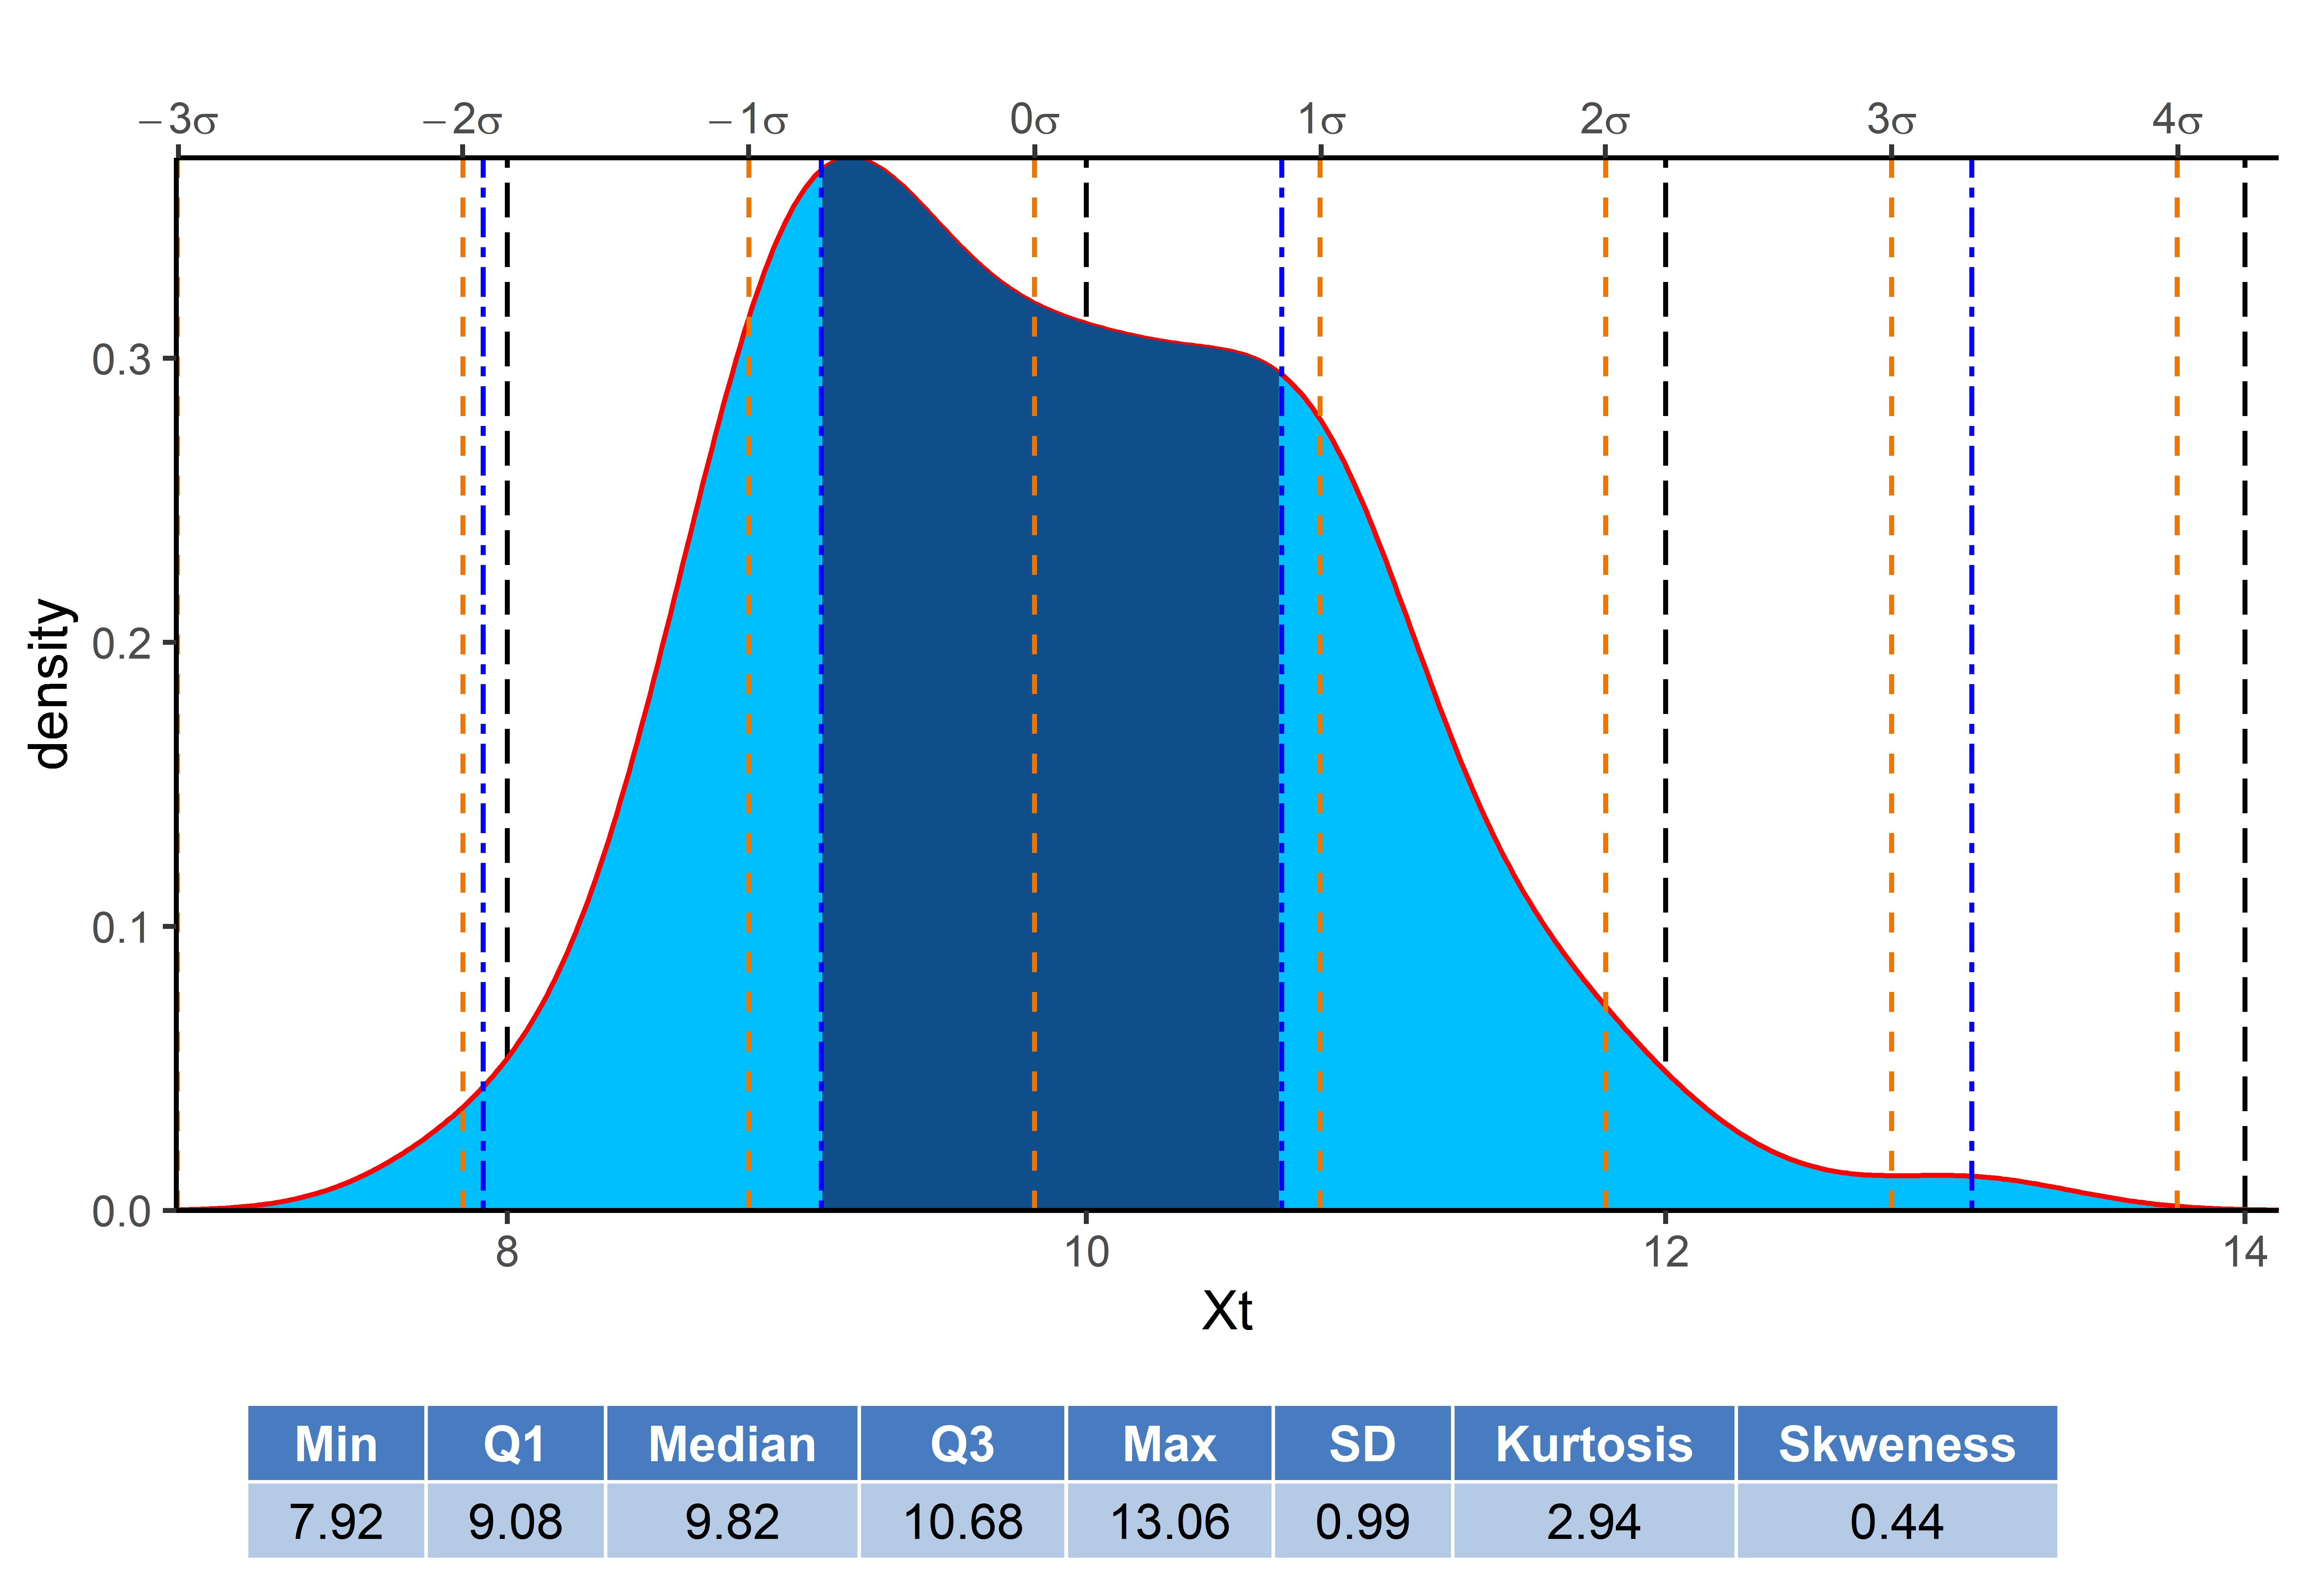
\includegraphics[width=1\linewidth,height=1\textheight]{Tesis_files/figure-latex/datos_simulados-1} \caption{Valores de referencia para la simulación de series cronológicas}\label{fig:datos_simulados}
\end{figure}

Por su lado, se simularon un total de ocho series cronológicas, cuyo
comportamiento y proceso gobernante se muestran en la figura
\ref{fig:series_simuladas}.

\begin{figure}[!h]
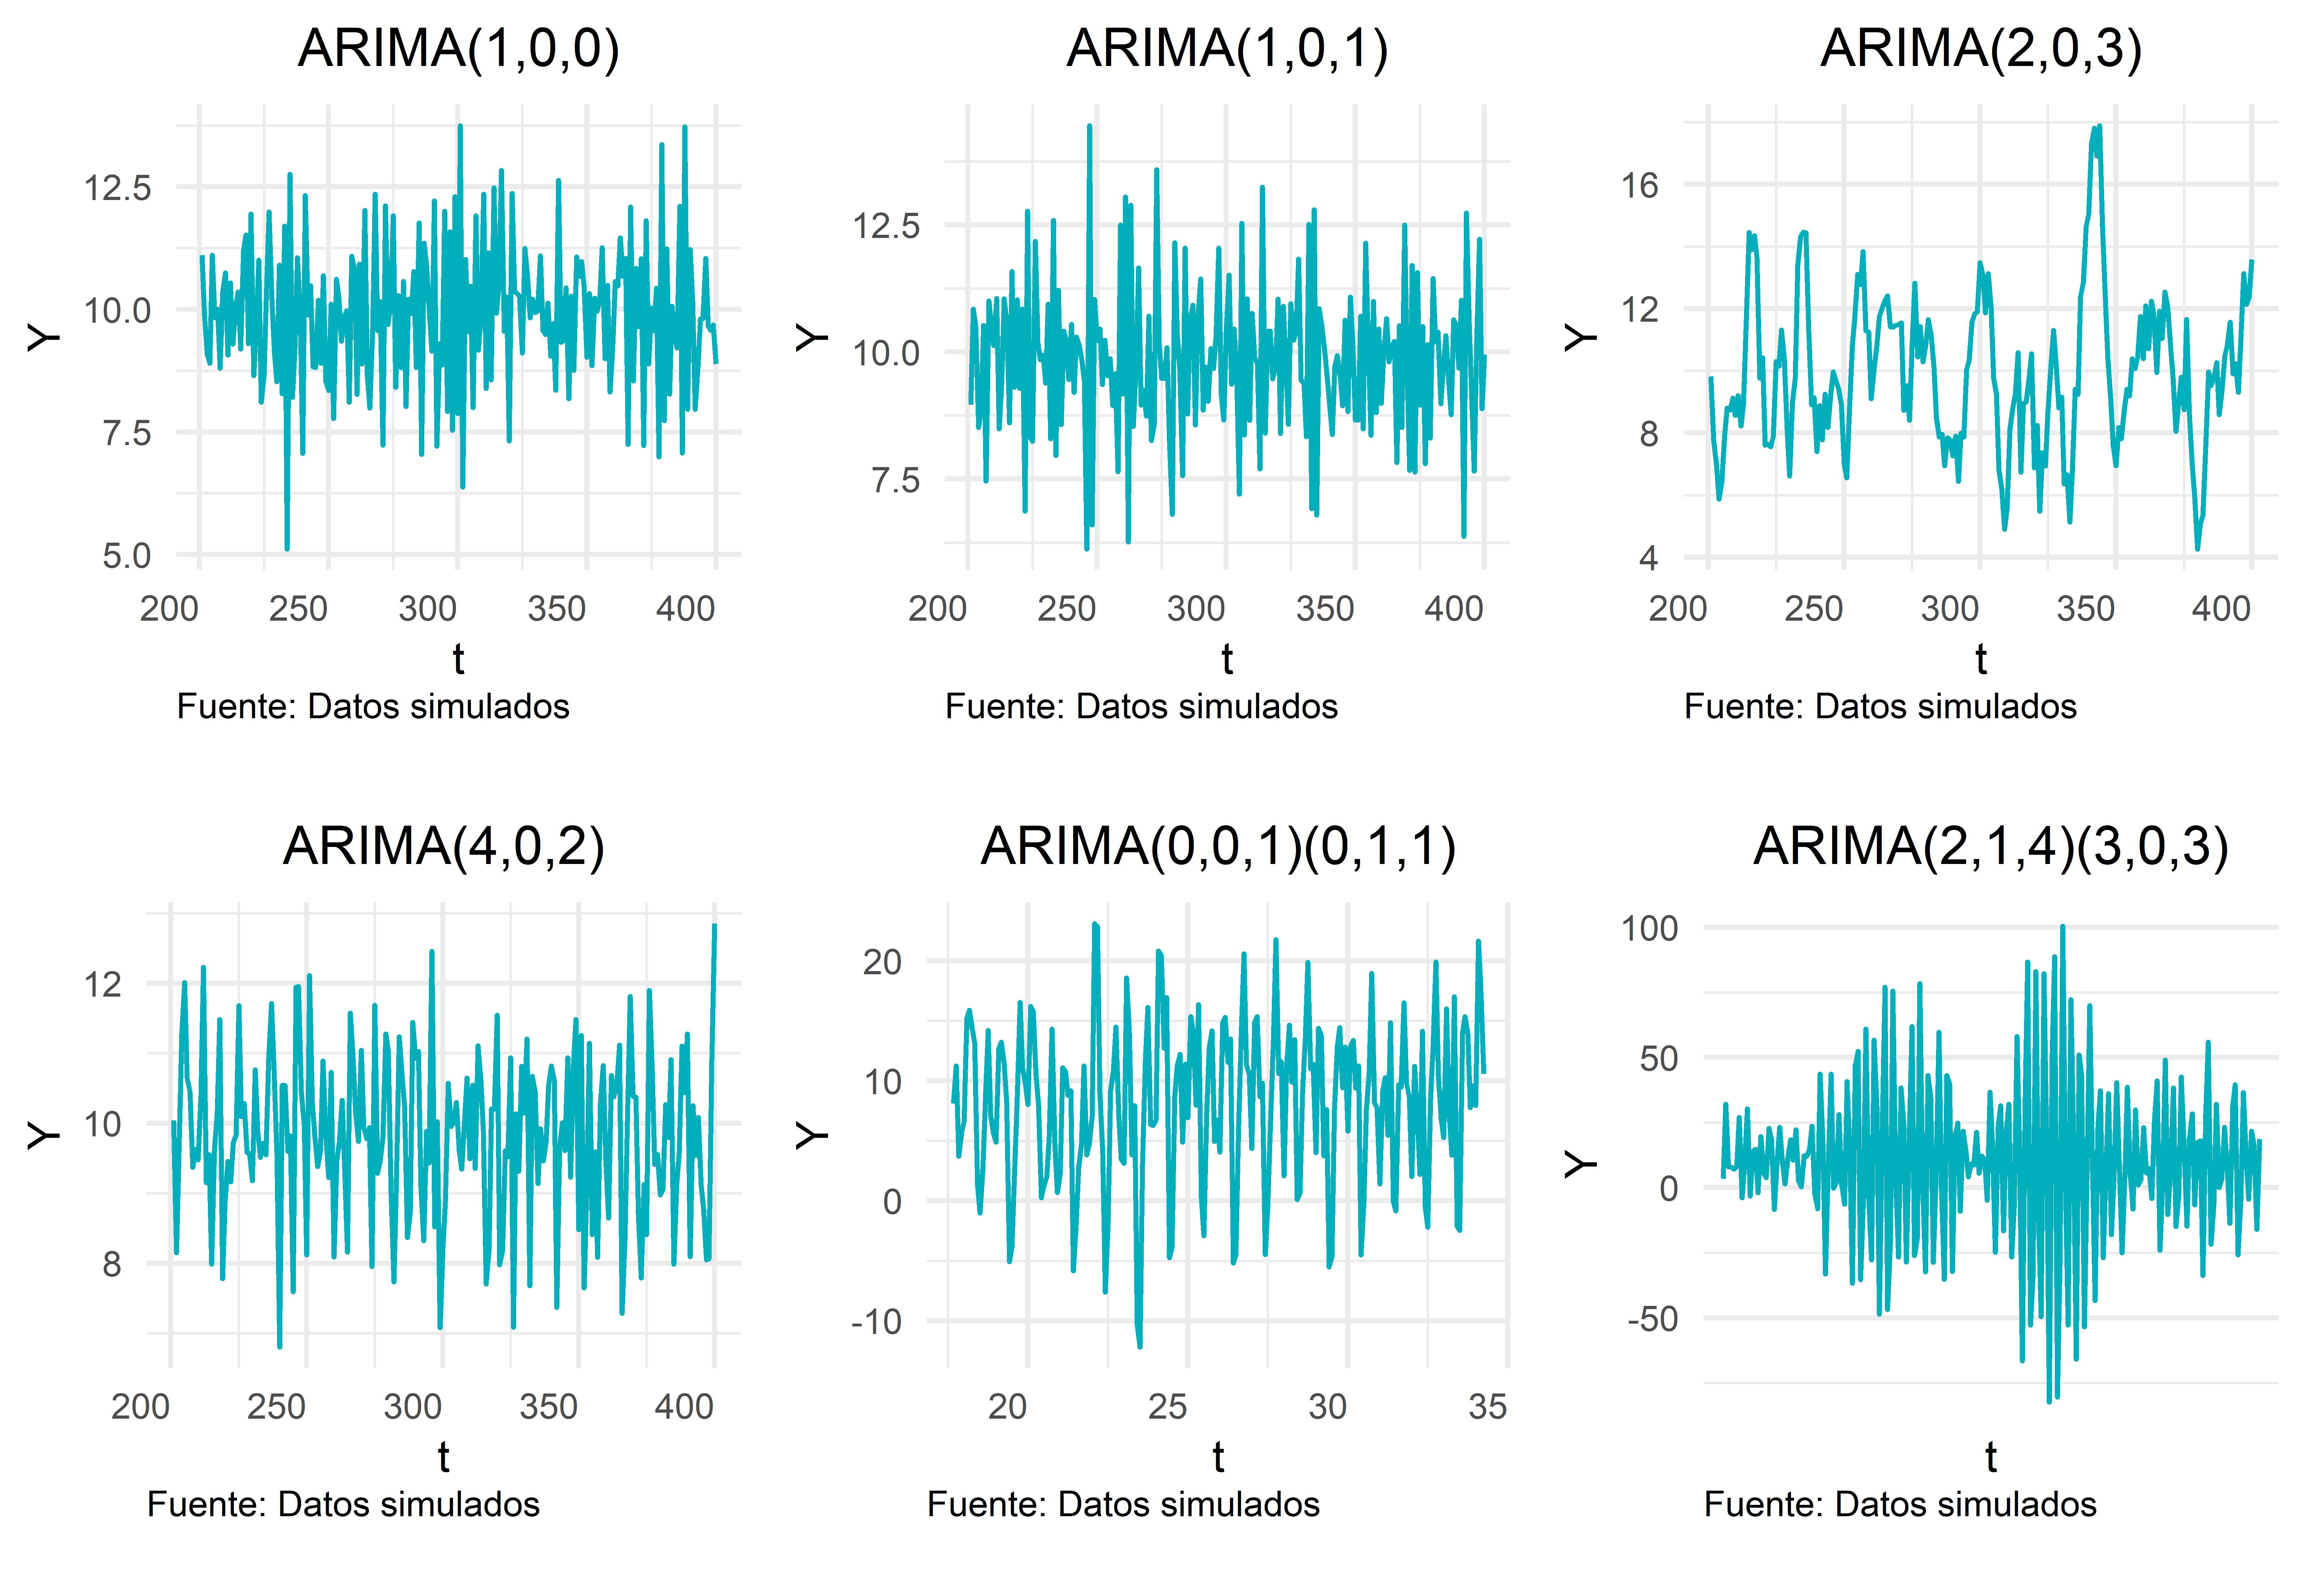
\includegraphics[width=1\linewidth,height=1\textheight]{Tesis_files/figure-latex/series_simuladas-1} \caption{Series cronológicas simuladas}\label{fig:series_simuladas}
\end{figure}

El cuadro \ref{tab:comparaciones} muestra los valores del MAE, MASE y
RMSE para cada proceso estimado y, además, muestra el proceso de origen
de las series cronológicas simuladas. Al aplicar la función
\texttt{auto.arima()} y la sobreparametrización sobre una serie
cronológica generada a partir de un \(ARIMA(1,0,0)\), se obtienen los
mismos resultados, y esto son ligeramente inferiores a los obtenidos
mediante un \(ARIMA(1,1,1)\). Al generar datos a partir de un
\(ARIMA(1,0,1)\) los mejores pronósticos se obtienen tanto con el
\texttt{auto.arima()} como con la sobreparametrización, pues ambos son
superiores a los obtenidos mediante un \(ARIMA(1,1,1)\). Al ir
incorporando términos en las series no estacionales, como es el caso de
los datos simulados a partir de un \(ARIMA(2,0,3)\), los mejores
pronósticos se obtienen mediante el uso de la sobreparametrización, pues
la magnitud de sus errores son siempre menores.

Cuando se consideran series cronológicas estacionales, se presenta un
comportamiento similar a lo previamente descrito. Al tener una baja
cantidad de parámetros en los datos simulados de un proceso estacional
\(ARIMA(0,0,1)(0,1,1)_{12}\), la sobreparametrización iguala los
resultados obtenidos mediante la función \texttt{auto.arima()}; y
además, cuando se incorporan más parámetros al modelo generador de los
dato como en el caso del \(ARIMA(2,1,4)(3,0,3)_{12}\), la
sobreparametrización logra captar de mejor manera el comportamiento de
los datos, obteniendo así menores mediciones del error, es decir, los
pronósticos se acercan más a los datos reales.

\begin{table}[!h]

\caption{\label{tab:unnamed-chunk-10}\label{tab:comparaciones}Medidas de rendimiento según método de estimación}
\centering
\resizebox{\linewidth}{!}{
\fontsize{5}{7}\selectfont
\begin{tabu} to \linewidth {>{\raggedleft\arraybackslash}p{2.5cm}>{\raggedleft\arraybackslash}p{2.5cm}>{\raggedleft}X>{\raggedleft}X>{\raggedleft}X>{\raggedleft}X}
\toprule
Proceso original & Método & Proceso & MAE & MASE & RMSE\\
\midrule
 & auto.arima & ARIMA(1,0,0) & 0.4942305 & 0.5528034 & 0.6402943\\
\cmidrule{2-6}
 & Sobreparametrización & ARIMA(1,0,0) & 0.4942305 & 0.5528034 & 0.6402943\\
\cmidrule{2-6}
\multirow{-3}{2.5cm}{\raggedleft\arraybackslash ARIMA(1,0,0)} & ARIMA estándar & ARIMA(1,1,1) & 0.4765113 & 0.5329843 & 0.6543140\\
\cmidrule{1-6}
 & auto.arima & ARIMA(0,0,1) & 0.8070104 & 0.5896820 & 1.1022758\\
\cmidrule{2-6}
 & Sobreparametrización & ARIMA(0,0,1) & 0.8070104 & 0.5896820 & 1.1022758\\
\cmidrule{2-6}
\multirow{-3}{2.5cm}{\raggedleft\arraybackslash ARIMA(1,0,1)} & ARIMA estándar & ARIMA(1,1,1) & 1.0726758 & 0.7838035 & 1.1821687\\
\cmidrule{1-6}
 & auto.arima & ARIMA(2,0,2) & 0.5128772 & 1.1656878 & 0.6699120\\
\cmidrule{2-6}
 & Sobreparametrización & ARIMA(5,1,1) & 0.4933922 & 1.1214016 & 0.6197431\\
\cmidrule{2-6}
\multirow{-3}{2.5cm}{\raggedleft\arraybackslash ARIMA(2,0,3)} & ARIMA estándar & ARIMA(1,1,1) & 0.5390294 & 1.2251276 & 0.6233500\\
\cmidrule{1-6}
 & auto.arima & ARIMA(2,0,3) & 0.5454557 & 1.1463361 & 0.7156326\\
\cmidrule{2-6}
 & Sobreparametrización & ARIMA(4,0,2) & 0.4570216 & 0.9604820 & 0.6649190\\
\cmidrule{2-6}
\multirow{-3}{2.5cm}{\raggedleft\arraybackslash ARIMA(4,0,2)} & ARIMA estándar & ARIMA(1,1,1) & 0.6131072 & 1.2885133 & 0.6860296\\
\cmidrule{1-6}
 & auto.arima & ARIMA(0,0,1)(0,1,1)[12] & 0.3877273 & 0.0547085 & 0.8137802\\
\cmidrule{2-6}
 & Sobreparametrización & ARIMA(0,0,1)(0,1,1)[12] & 0.3877273 & 0.0547085 & 0.8137802\\
\cmidrule{2-6}
\multirow{-3}{2.5cm}{\raggedleft\arraybackslash ARIMA(0,0,1)(0,1,1)[12]} & ARIMA estándar & ARIMA(1,1,1)(1,1,1)[12] & 0.3941180 & 0.0556102 & 0.9030985\\
\cmidrule{1-6}
 & auto.arima & ARIMA(2,0,4)(0,0,2)[12] & 3.6020919 & 0.1811366 & 4.8015578\\
\cmidrule{2-6}
 & Sobreparametrización & ARIMA(2,1,3)(0,1,3)[12] & 3.5539765 & 0.1787170 & 4.7836465\\
\cmidrule{2-6}
\multirow{-3}{2.5cm}{\raggedleft\arraybackslash ARIMA(2,1,4)(3,0,3)[12]} & ARIMA estándar & ARIMA(1,1,1)(1,1,1)[12] & 9.6771221 & 0.4866286 & 14.3620737\\
\bottomrule
\end{tabu}}
\end{table}

\subsection{Estimaciones en series cronológicas costarricenses reales}

\subsubsection{Tasa de mortalidad infantil interanual}

La Tasa de Mortalidad Infantil (TMI) es uno de los indicadores
demográficos más importantes, pues es utilizado como un parámetro de
referencia sobre la calidad del sistema de salud, tanto a nivel nacional
como regional. Si bien este indicador se construye relacionando las
defunciones de menores de un año con el total de nacimientos, también
involucra de manera implícita otras condiciones tales como las
económicas, sociales y culturales, así como la efectividad en los
métodos preventivos y curativos de esta categoría poblacional
(\protect\hyperlink{ref-leon}{León, 1998}). Debido a esto, el
fallecimiento de un niño menor de un año se traduce en una falla del
sistema de salud, por lo que estos casos son sujetos de estudio con el
fin de conocer las causas que desencadenaron el evento.

En algunos países en vías de desarrollo de Asia, África y América
Latina, la mortalidad infantil alcanza valores elevados pues la
desnutrición, ausencia de asistencia médica y mala calidad de las
condiciones sanitarias son, a diferencia de los países más
desarrollados, algo muy común (\protect\hyperlink{ref-donoso}{Donoso,
2004}). En el caso de Costa Rica, la unidad de estadísticas demográficas
del Instituto Nacional de Estadística y Censos\footnote{\url{http://www.inec.go.cr/}}
(INEC) es el ente encargado de reportar este indicador con el fin de dar
seguimiento y control al comportamiento del mismo a lo largo del tiempo
con el objetivo de llegar a los niveles más bajos posibles.

En el INEC, cada mes se publica el boletín de la TMI interanual (TMII),
que analiza la TMI de un mes y los 11 meses previos para comparar los
periodos correspondientes (\protect\hyperlink{ref-infantiles}{INEC,
2004}). Este apartado busca hacer un análisis de la TMII para los 12
periodos desde el año 1989 y hasta 2017, y no de manera mensual simple,
pues dada la volatilidad del fenómeno de estudio, hacer un estudio
interanual permite analizar de una mejor manera los cambios entre
periodos. Es decir, se analizará la TMII desde el periodo Febrero 1989
-- Enero 1990 hasta el periodo Enero 2017 -- Diciembre 2017.

La importancia de este proceso, aparte de servir de parámetro para
evaluar el sistema de salud, está en su estrecha relación con las
proyecciones de población, pues como se mencionó previamente, la TMII
analiza la mortalidad en el grupo de edad de menores de un año, que es
el primer grupo al generar tablas de mortalidad, ya sea de la forma
clásica o mediante la mortalidad óptima
(\protect\hyperlink{ref-mortalidad_optima}{Villalón, 2006}). Uno de los
métodos más conocidos para realizar estas estimaciones es el método de
los componentes de cambio demográfico, que son la fecundidad, la
mortalidad y la migración. En el caso de la mortalidad, uno de los
puntos de partida es la estimación de las tasas de mortalidad por grupos
de edad, siendo de particular interés la de menores de cinco años, pues
esta a su vez se subdivide en los grupos de menores de un año y el de
uno a cuatro años. Conocer el comportamiento de la mortalidad infantil
es importante porque es en este grupo de edad en el que pueden existir
cambios muy bruscos en la mortalidad y la fecundidad
(\protect\hyperlink{ref-Rincon}{Rincon, 2000}).

Dado que la medición de la TMII se hace partiendo de un determinado mes
y a partir de éste se consideran los 11 meses anteriores, el primer
valor de la base de datos fue medido a partir de Enero de 2000, que
corresponde al período interanual Febrero 1999 -- Enero 2000. Todos los
periodos siguientes se muestran en la figura \ref{fig:tmiiplotgeneral}.

\begin{figure}[!h]
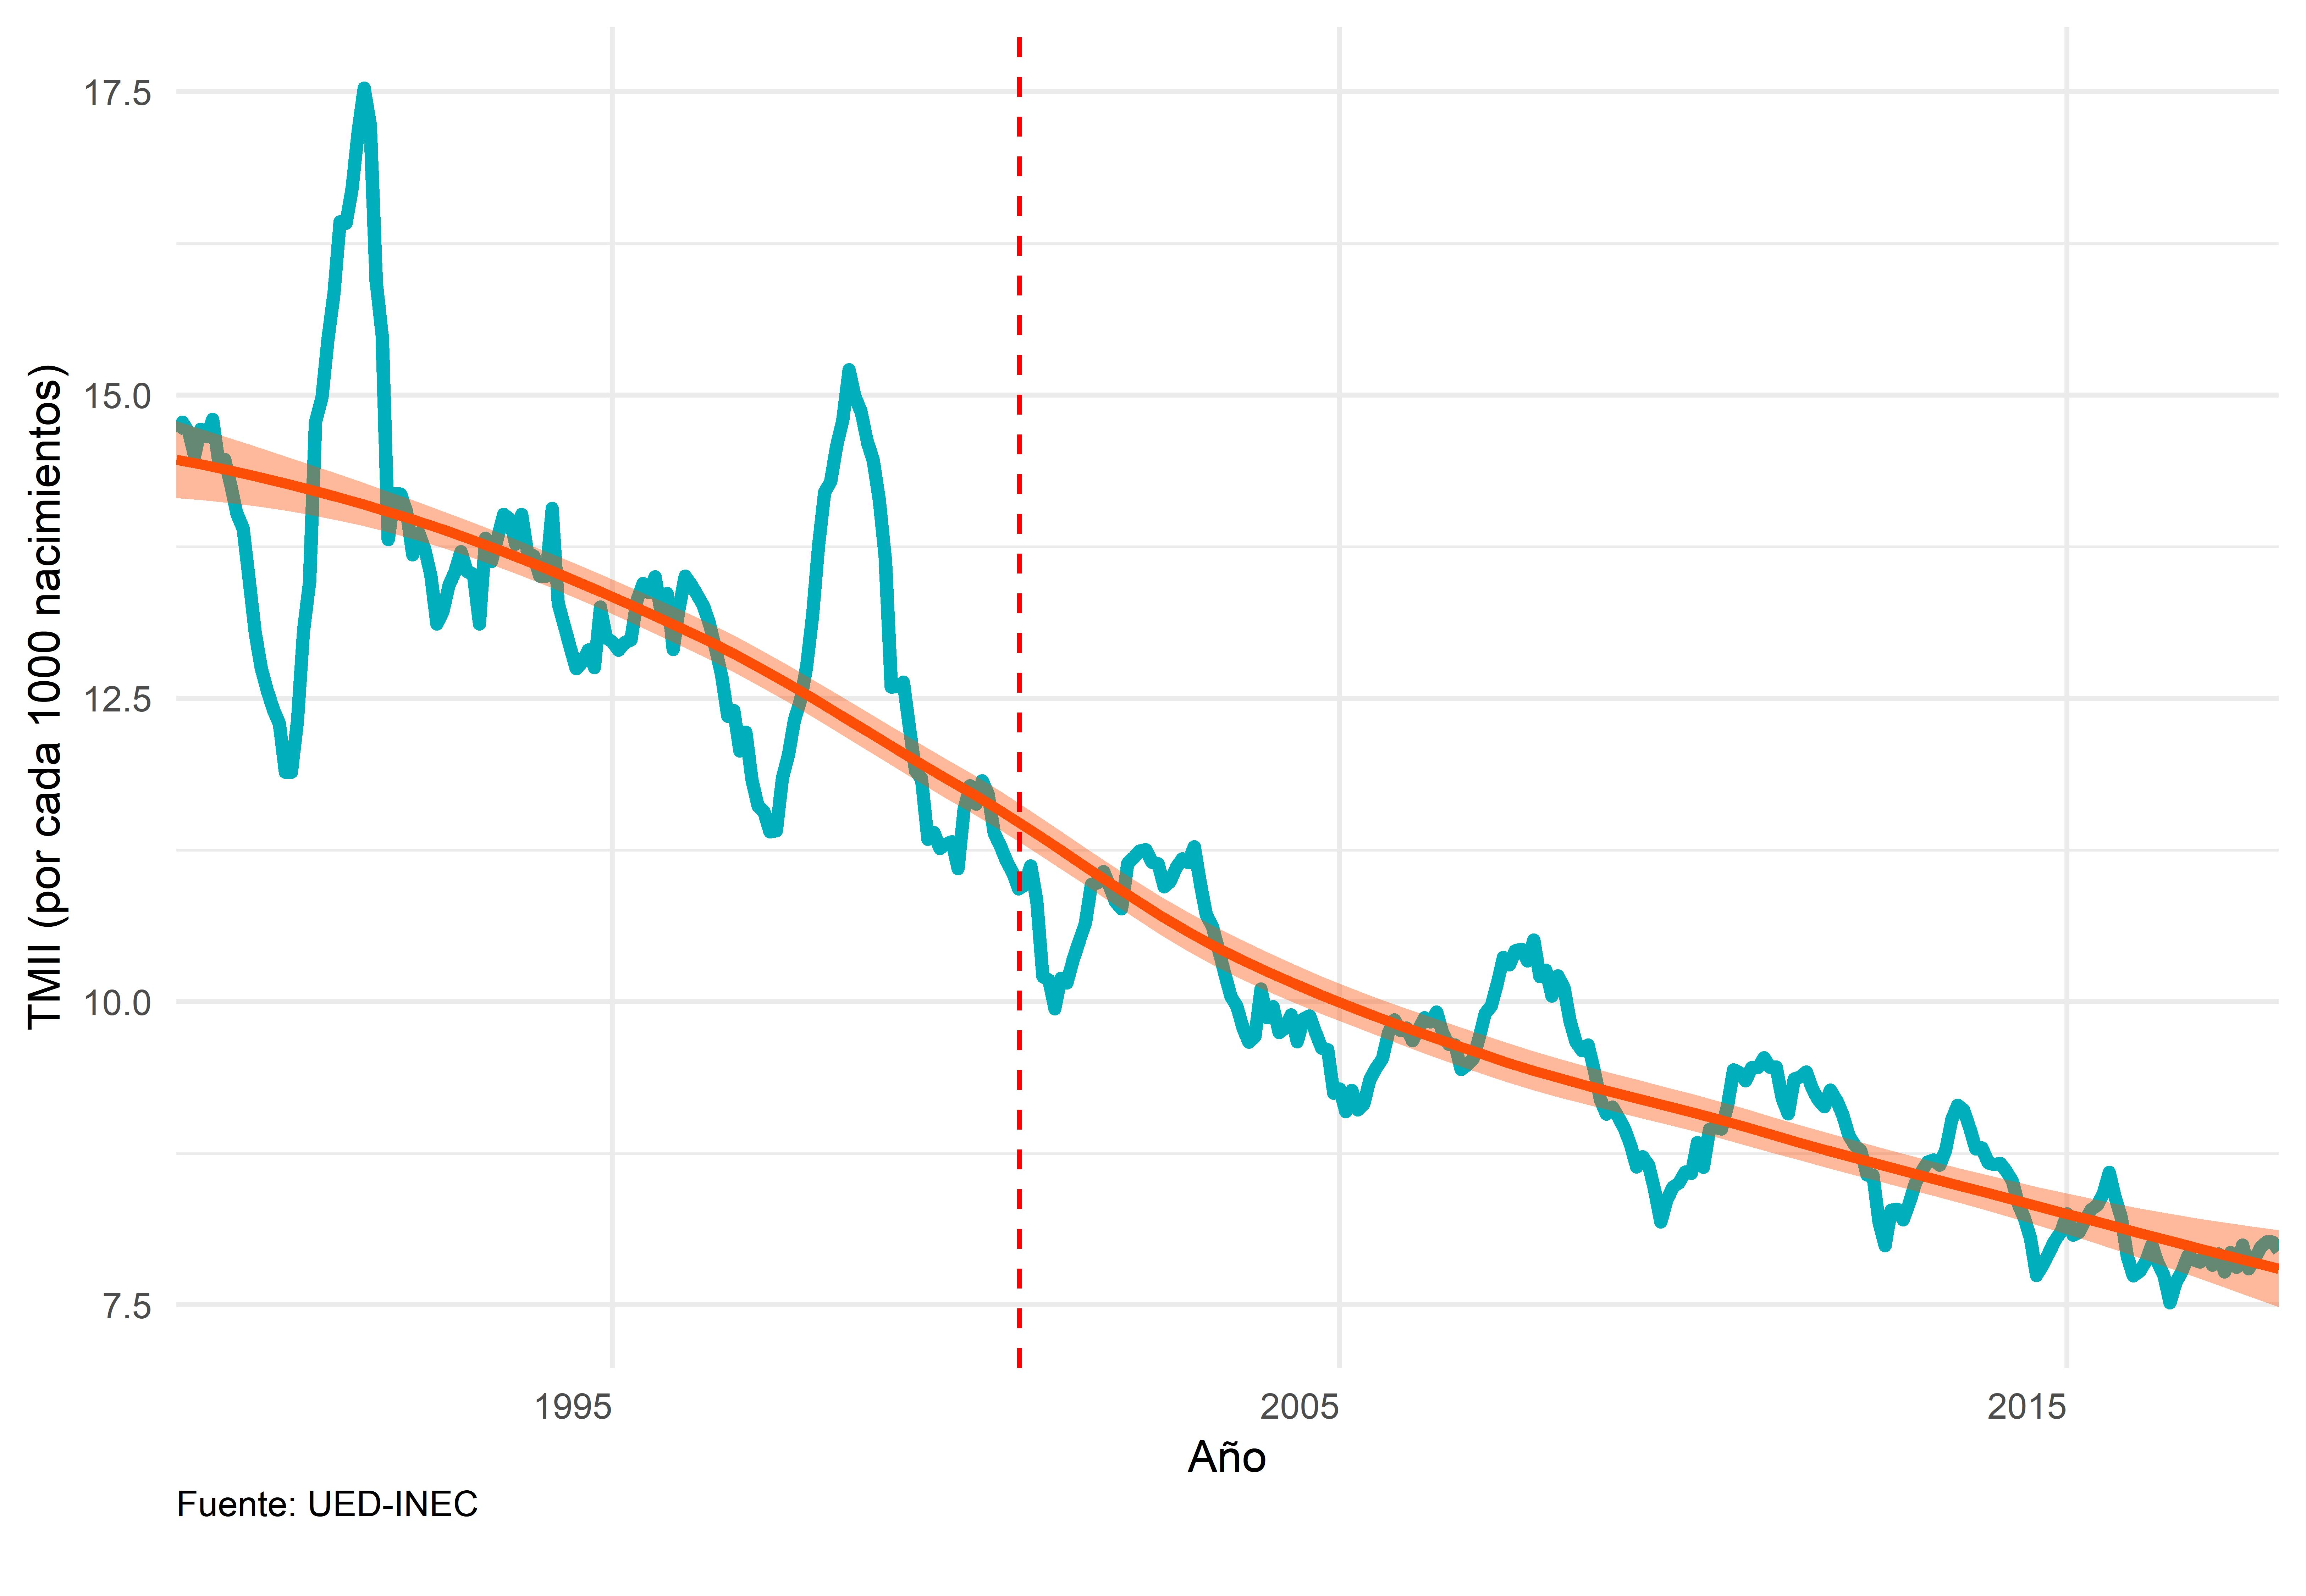
\includegraphics[width=1\linewidth,height=1\textheight]{Tesis_files/figure-latex/tmiiplotgeneral-1} \caption{Tasa de Mortalidad Infantil Interanual 1989 - 2017}\label{fig:tmiiplotgeneral}
\end{figure}

La serie muestra picos y valles pronunciados a lo largo de todo el
periodo. A modo de visualización, se ajustó un suavizamiento de Loess
para buscar señales de tendencia y concavidad en los datos temporales.
La línea roja punteada se ubica aproximadamente en el mes de Julio del
año 2000, pues a partir de ese punto el suavizamiento de Loess muestra
un ligero cambio en la concavidad, lo cual sugiere que a partir ese
punto será más difícil que la TMII vuelva a alcanzar valores similares a
los mostrados al inicio de la serie. Además, al presentarse dos caídas y
subidas abruptas en la TMII, esta tiende a estabilizarse.

Mediante un análisis visual, la figura \ref{fig:tmiiplotperiodos} parece
respaldar el supuesto de que la mortalidad no posee efectos estacionales
determinantes, pues para cada uno de los 12 períodos, en ninguno parecen
existir mayores diferencias. El efecto que se mantiene en cada uno de
los períodos es el de la tendencia, pues en cada uno ésta sigue
descendiendo con el pasar de los años. Este hecho coincide con lo
observado en la figura \ref{fig:tmiiplotgeneral}.

\begin{figure}[!h]
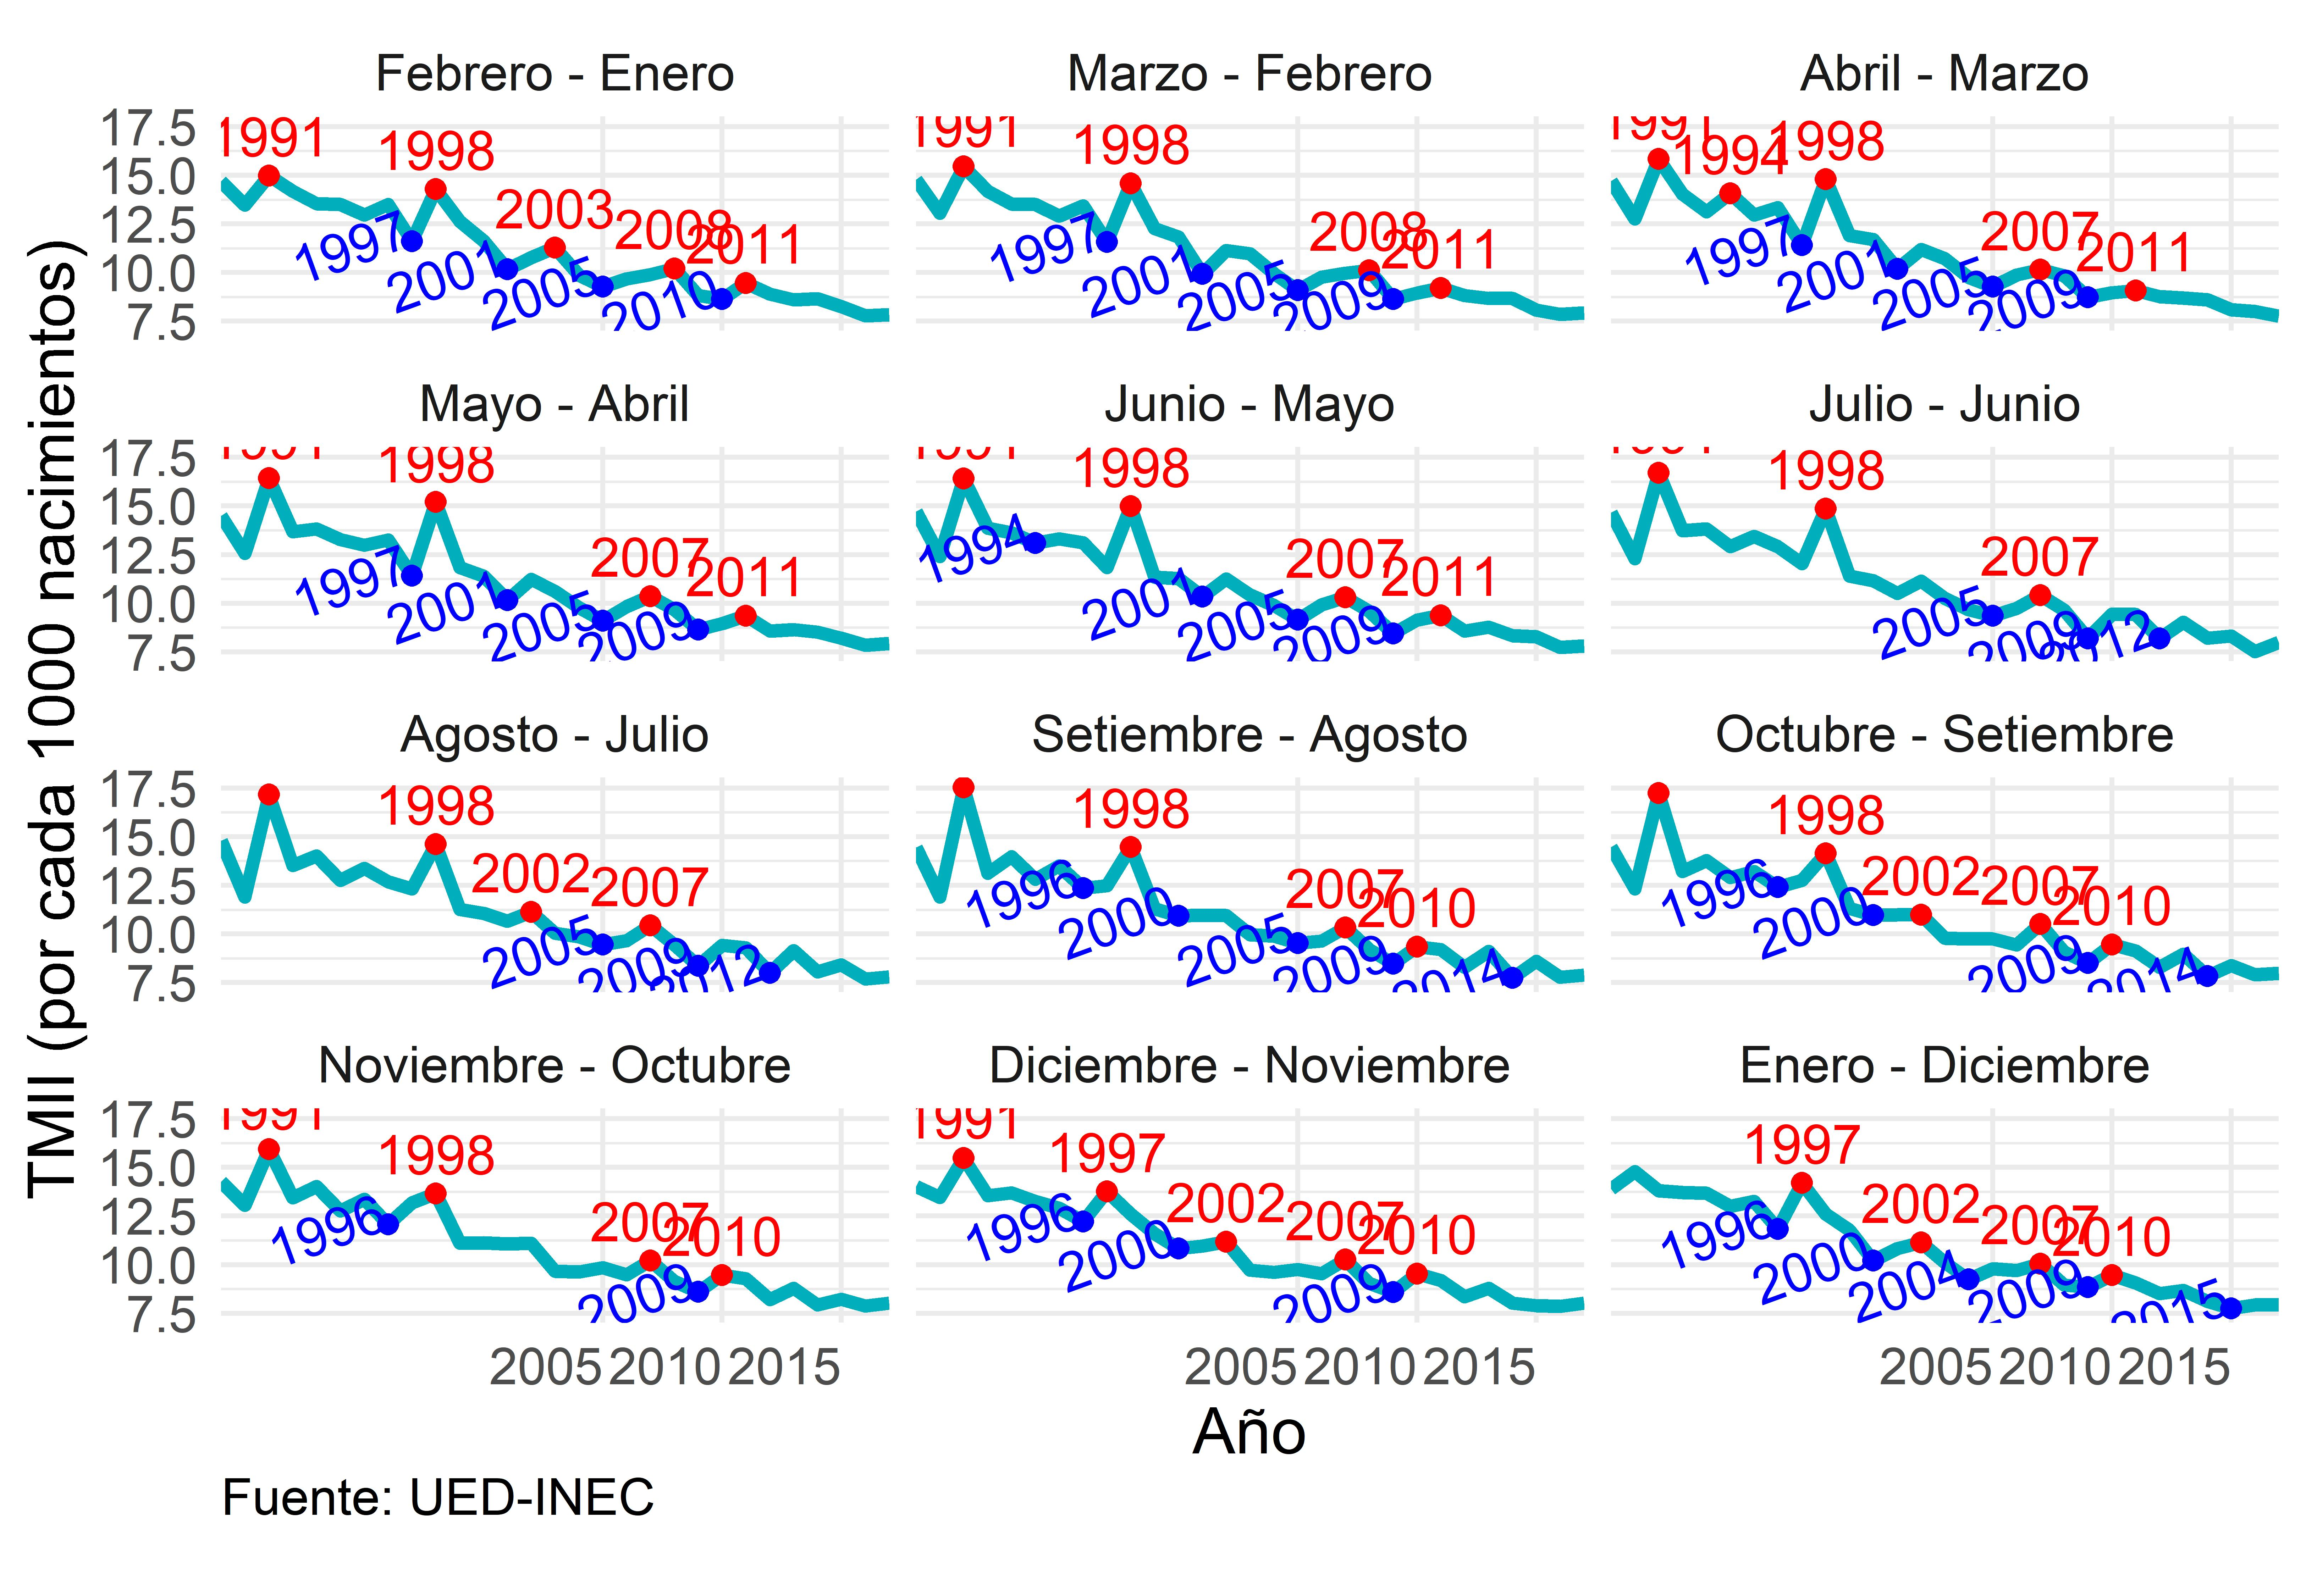
\includegraphics[width=1\linewidth,height=1\textheight]{Tesis_files/figure-latex/tmiiplotperiodos-1} \caption{Tasa de Mortalidad Infantil Interanual 1989 - 2017 según periodos}\label{fig:tmiiplotperiodos}
\end{figure}

Para hacer la descomposición de la serie se hizo una transformación de
Box-Cox con \(\lambda=1\) para aplicarla de manera multiplicativa. Esto
se debe a que en la figura \ref{fig:tmiiplotgeneral} pueden observarse
cambios considerables en la variabilidad de la serie a lo largo del
tiempo. la figura \ref{fig:tmiiplotdescomposicion} muestra, como se
mencionó previamente, una tendencia decreciente y una estacionalidad que
no es reiterada a lo largo del tiempo. Además, el componente aleatorio
muestra como los errores no son constantes durante todo el período.

\begin{figure}[!h]
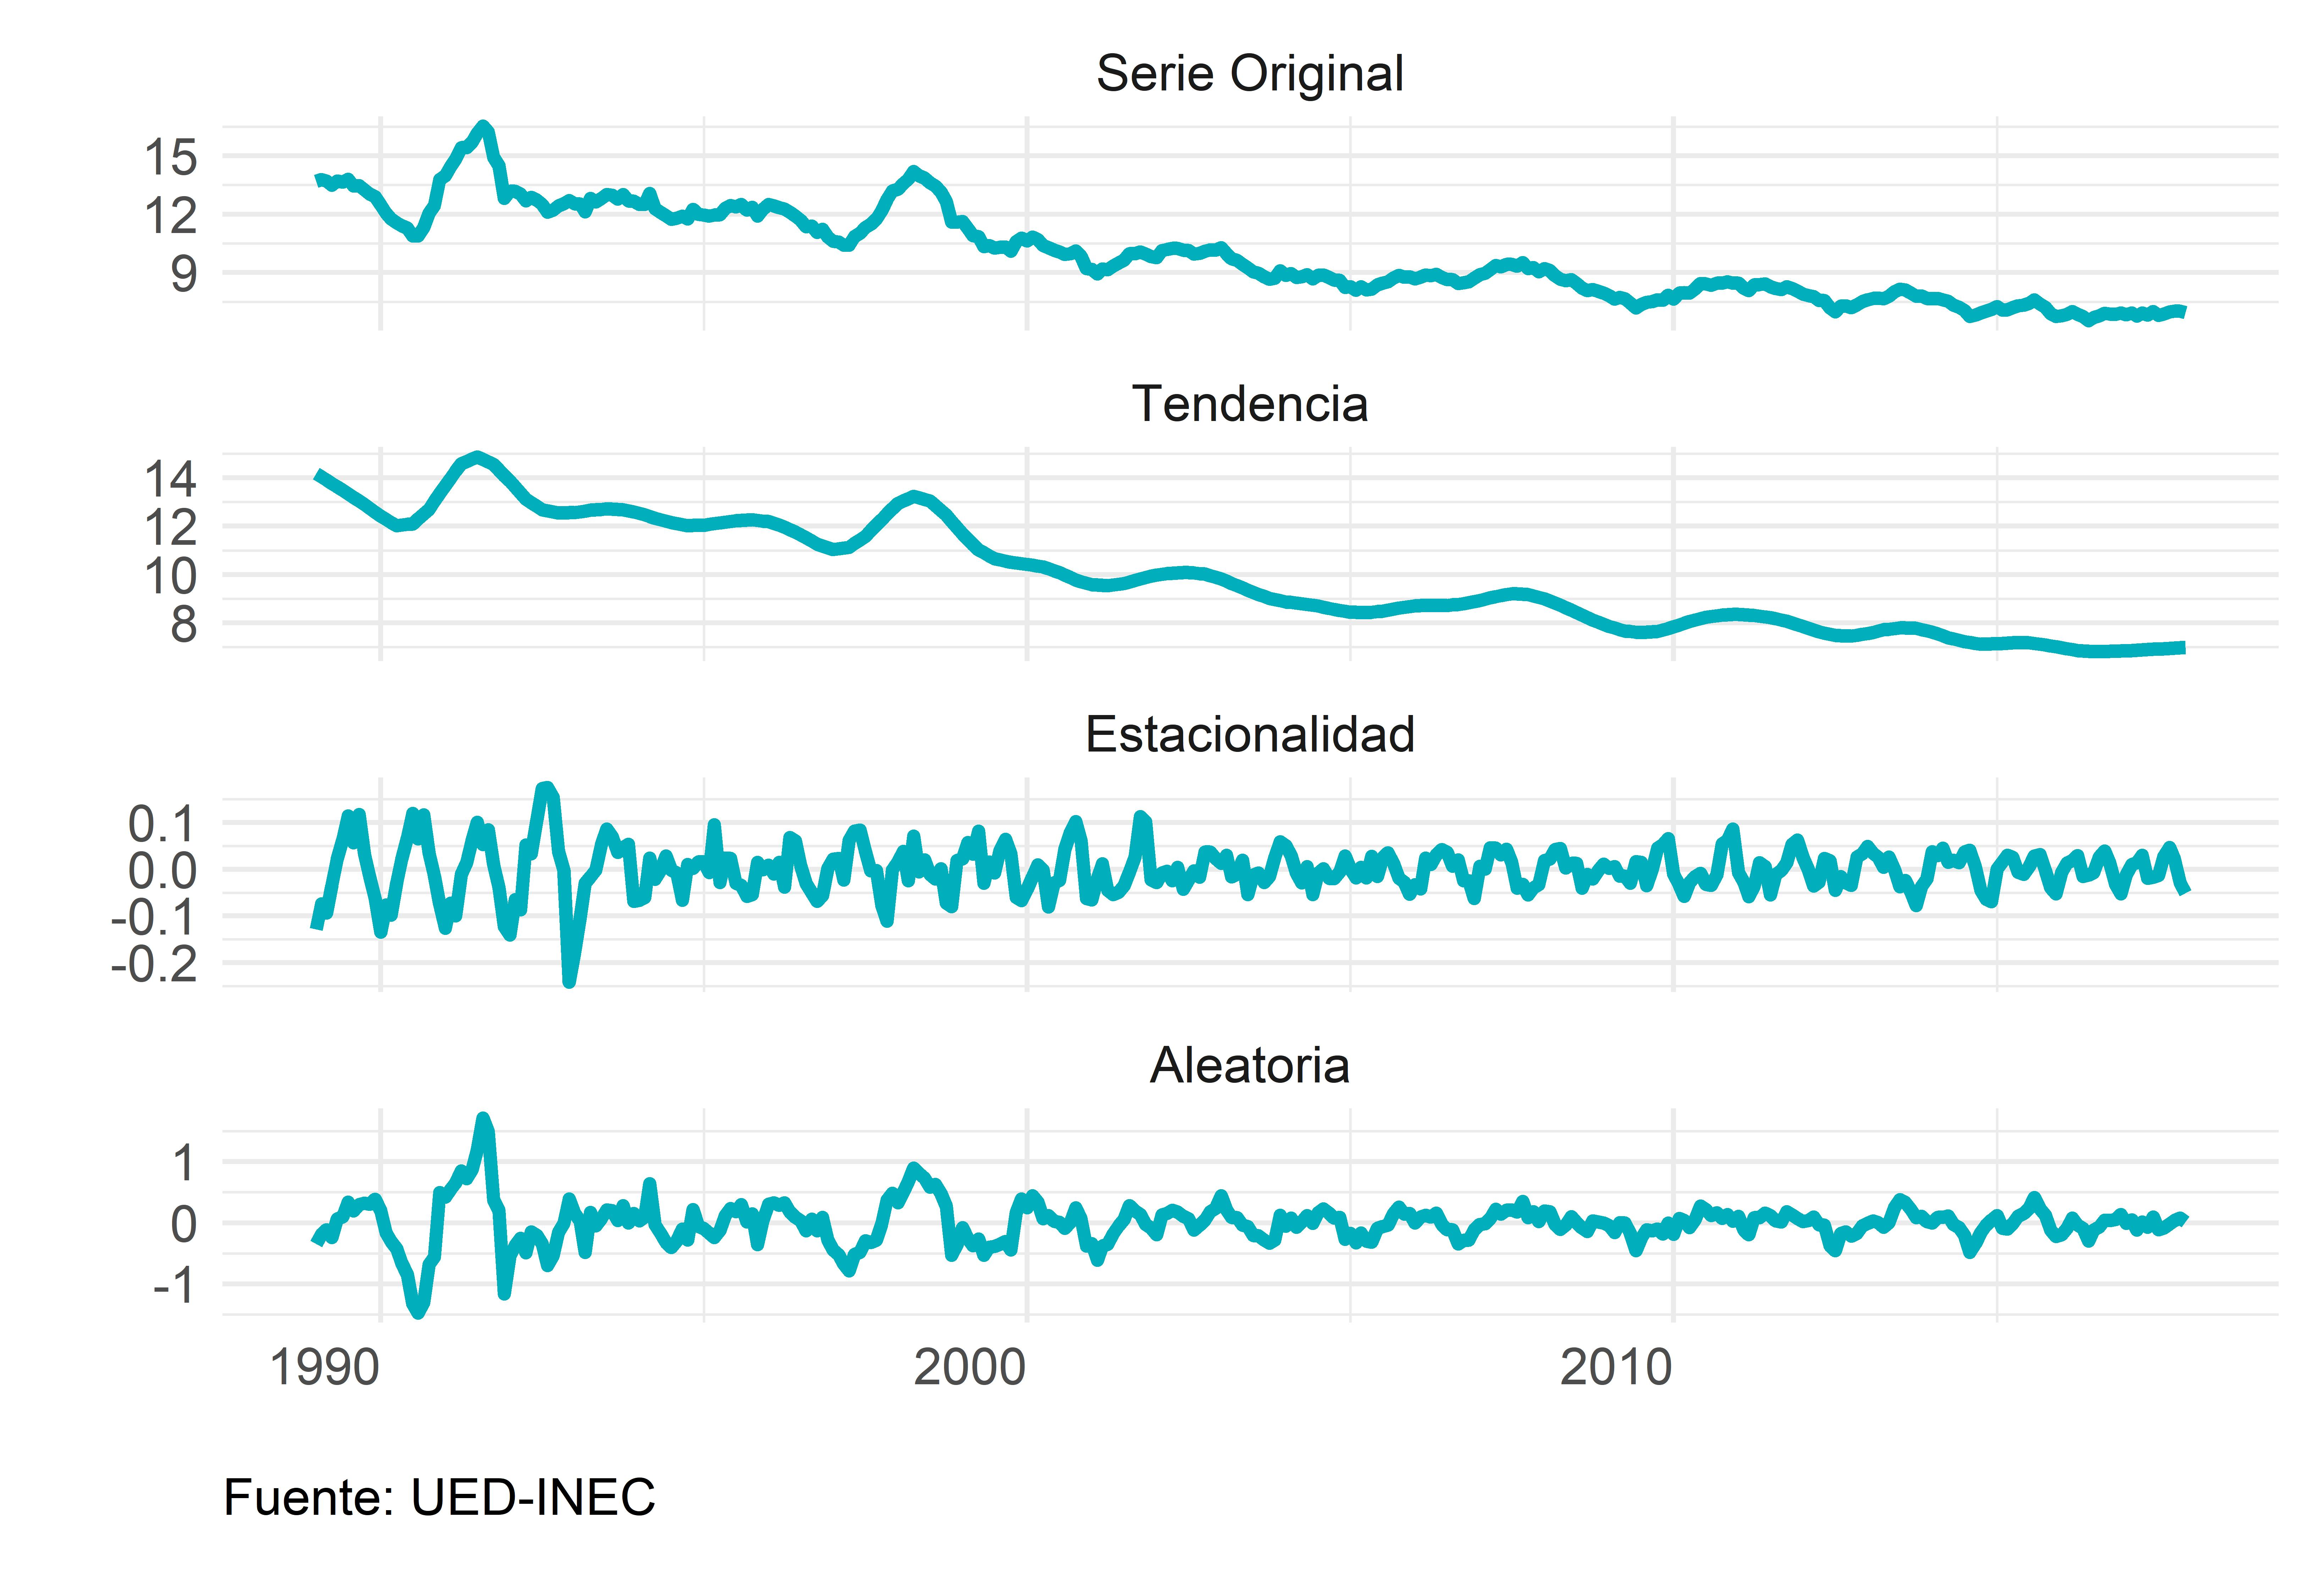
\includegraphics[width=1\linewidth,height=1\textheight]{Tesis_files/figure-latex/tmiiplotdescomposicion-1} \caption{Descomposición de la TMII en el periodo 2000 - 2017}\label{fig:tmiiplotdescomposicion}
\end{figure}

Tras tener un panorama más claro del comportamiento de la serie mediante
el análisis descriptivo anterior, se modela la serie mediante la función
\texttt{auto.arima()}, teniendo como mejor modelo un
\(ARIMA(2,1,0)(0,0,1)\); y utilizando la sobreparametrización se tiene
como mejor modelo un \(ARIMA(4,1,0)(4,1,0)\). El cuadro
\ref{tab:tmiimedidas} muestra como el uso de la sobreparametrización
ofrece pronósticos más cercanos al valor real, y aunque los pronósticos
están lejos de ser perfectos, el método propuesto logra reproducir de
mejor manera el comportamiento de los datos, tal y como se muestra en la
figura \ref{fig:tmiiplotpronostico}

\begin{table}[!h]

\caption{\label{tab:unnamed-chunk-13}\label{tab:tmiimedidas}Medidas de rendimiento según método de estimación para la TMII}
\centering
\resizebox{\linewidth}{!}{
\begin{tabu} to \linewidth {>{\raggedleft}X>{\raggedleft}X>{\raggedleft}X>{\raggedleft}X}
\toprule
Método & RMSE & MAE & MAPE\\
\midrule
autoarima & 1.1481936 & 1.0192497 & 12.683182\\
sobreparametrizacion & 0.3495541 & 0.2839742 & 3.418392\\
\bottomrule
\end{tabu}}
\end{table}

\begin{figure}[!h]
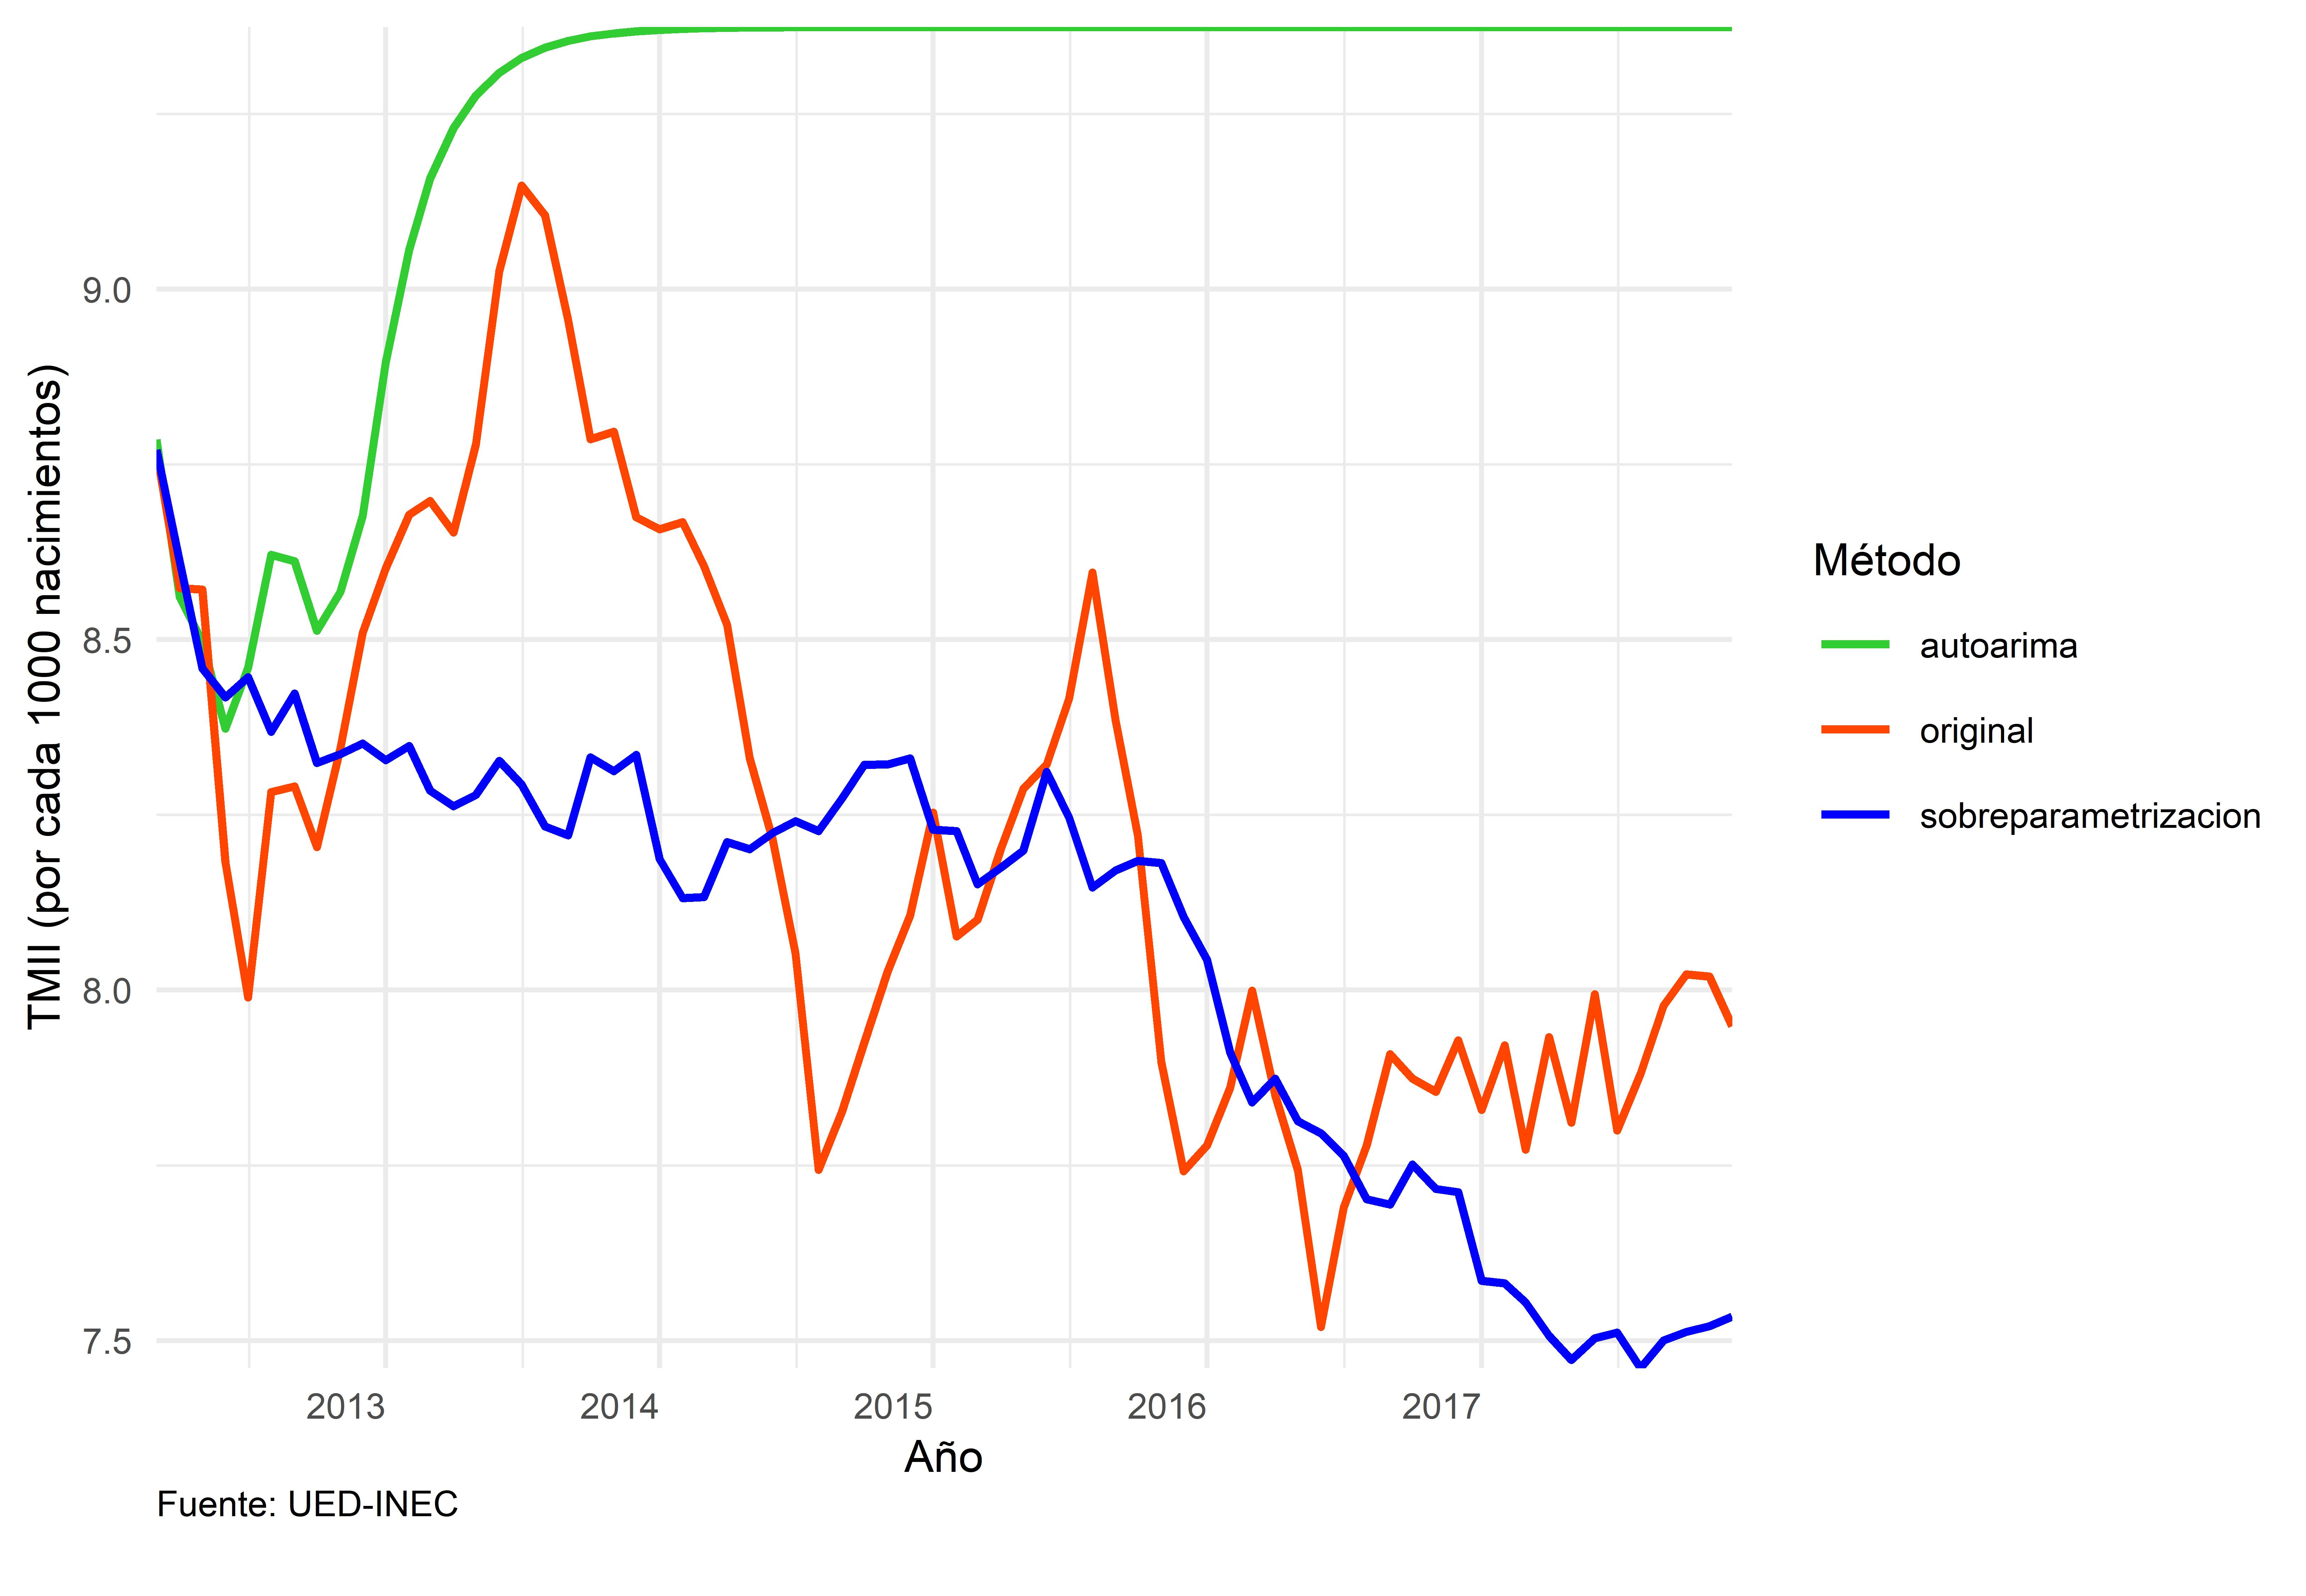
\includegraphics[width=1\linewidth,height=1\textheight]{Tesis_files/figure-latex/tmiiplotpronostico-1} \caption{Pronósticos de la TMII según método de estimación}\label{fig:tmiiplotpronostico}
\end{figure}

\subsubsection{Mortalidad por causa externa}

La violencia es un acto tan antiguo como el mundo, sin embargo, la
evolución de esta en conjunto con el crecimiento de su relación con las
defunciones registradas en una población la vuelven un problema de salud
pública. En base a la clasificación Internacional de Enfermedades
(\protect\hyperlink{ref-CIE10}{OPS, 2016}) de la de la Organización
Mundial de la Salud\footnote{\url{https://www.paho.org/salud-en-las-americas-2017/?lang=es}{]}},
las defunciones pueden clasificarse en cuatro grandes grupos, siendo el
más importante el de las causas naturales, el cual incluye enfermedades
congénitas, cardiopatías u otras relacionadas con la vejez. En menor
cuantía se encuentran las causas de muerte ignoradas, las cuales se dan
cuando la causa de muerte es desconocida y de intención indeterminada; y
de forma similar se encuentran las causas de muerte que se mantienen en
estudio, bien sea por parte de la morgue o de algún otro organismo, esta
última tiene pocos registros conforme más se retrocede en el tiempo.

El otro gran grupo, aunque considerablemente menor que las causas
naturales, son las causas externas, las cuales son objeto de análisis en
este apartado. Este grupo puede a su vez ser clasificado en homicidios,
suicidios y las muertes accidentales, esta última comprende los
accidentes de tránsito, las muertes por caídas, personas ahogadas,
víctimas de incendios, terraplenes u otros similares. Aunado a estas
categorías se encuentran también las causas indeterminadas, las cuales
se diferencian a las ignoradas en que se sabe que se debe a una causa
externa pero no se conoce con certeza a cuál categoría pertenece o aún
está en investigación, tal es el caso de una persona que fallece debido
a una alta ingesta de drogas o estupefacientes; bien pudo haber
consumido intencionalmente hasta morir, lo cual sería un suicidio, o
bien el consumo excesivo se debió a un accidente.

En Costa Rica para el año 2011, las muertes por causas externas ocuparon
el tercer lugar, siendo solo superadas por las enfermedades del sistema
circulatorio, en particular las enfermedades cardiovasculares, y los
tumores, ambos casos mostraron una tendencia ascendente
(\protect\hyperlink{ref-nacion}{Nación, 2013}). Es debido a los elevados
costos económicos y sociales
(\protect\hyperlink{ref-ccpexternas}{Cardona, 2013}) que se aborda la
imperiosa necesidad comprender el comportamiento de las defunciones
debido a las causas externas con el fin de contar con un punto de
partida para la elaboración de políticas públicas que busquen reducir al
mínimo este tipo de eventos.

Dado que los registros de defunciones por causa externa se realizan
diariamente, conviene analizar su comportamiento de manera mensual desde
inicios del milenio de una manera más general, dicho comportamiento
puede observarse en la figura \ref{fig:externaplotgeneral}.

\begin{figure}[!h]
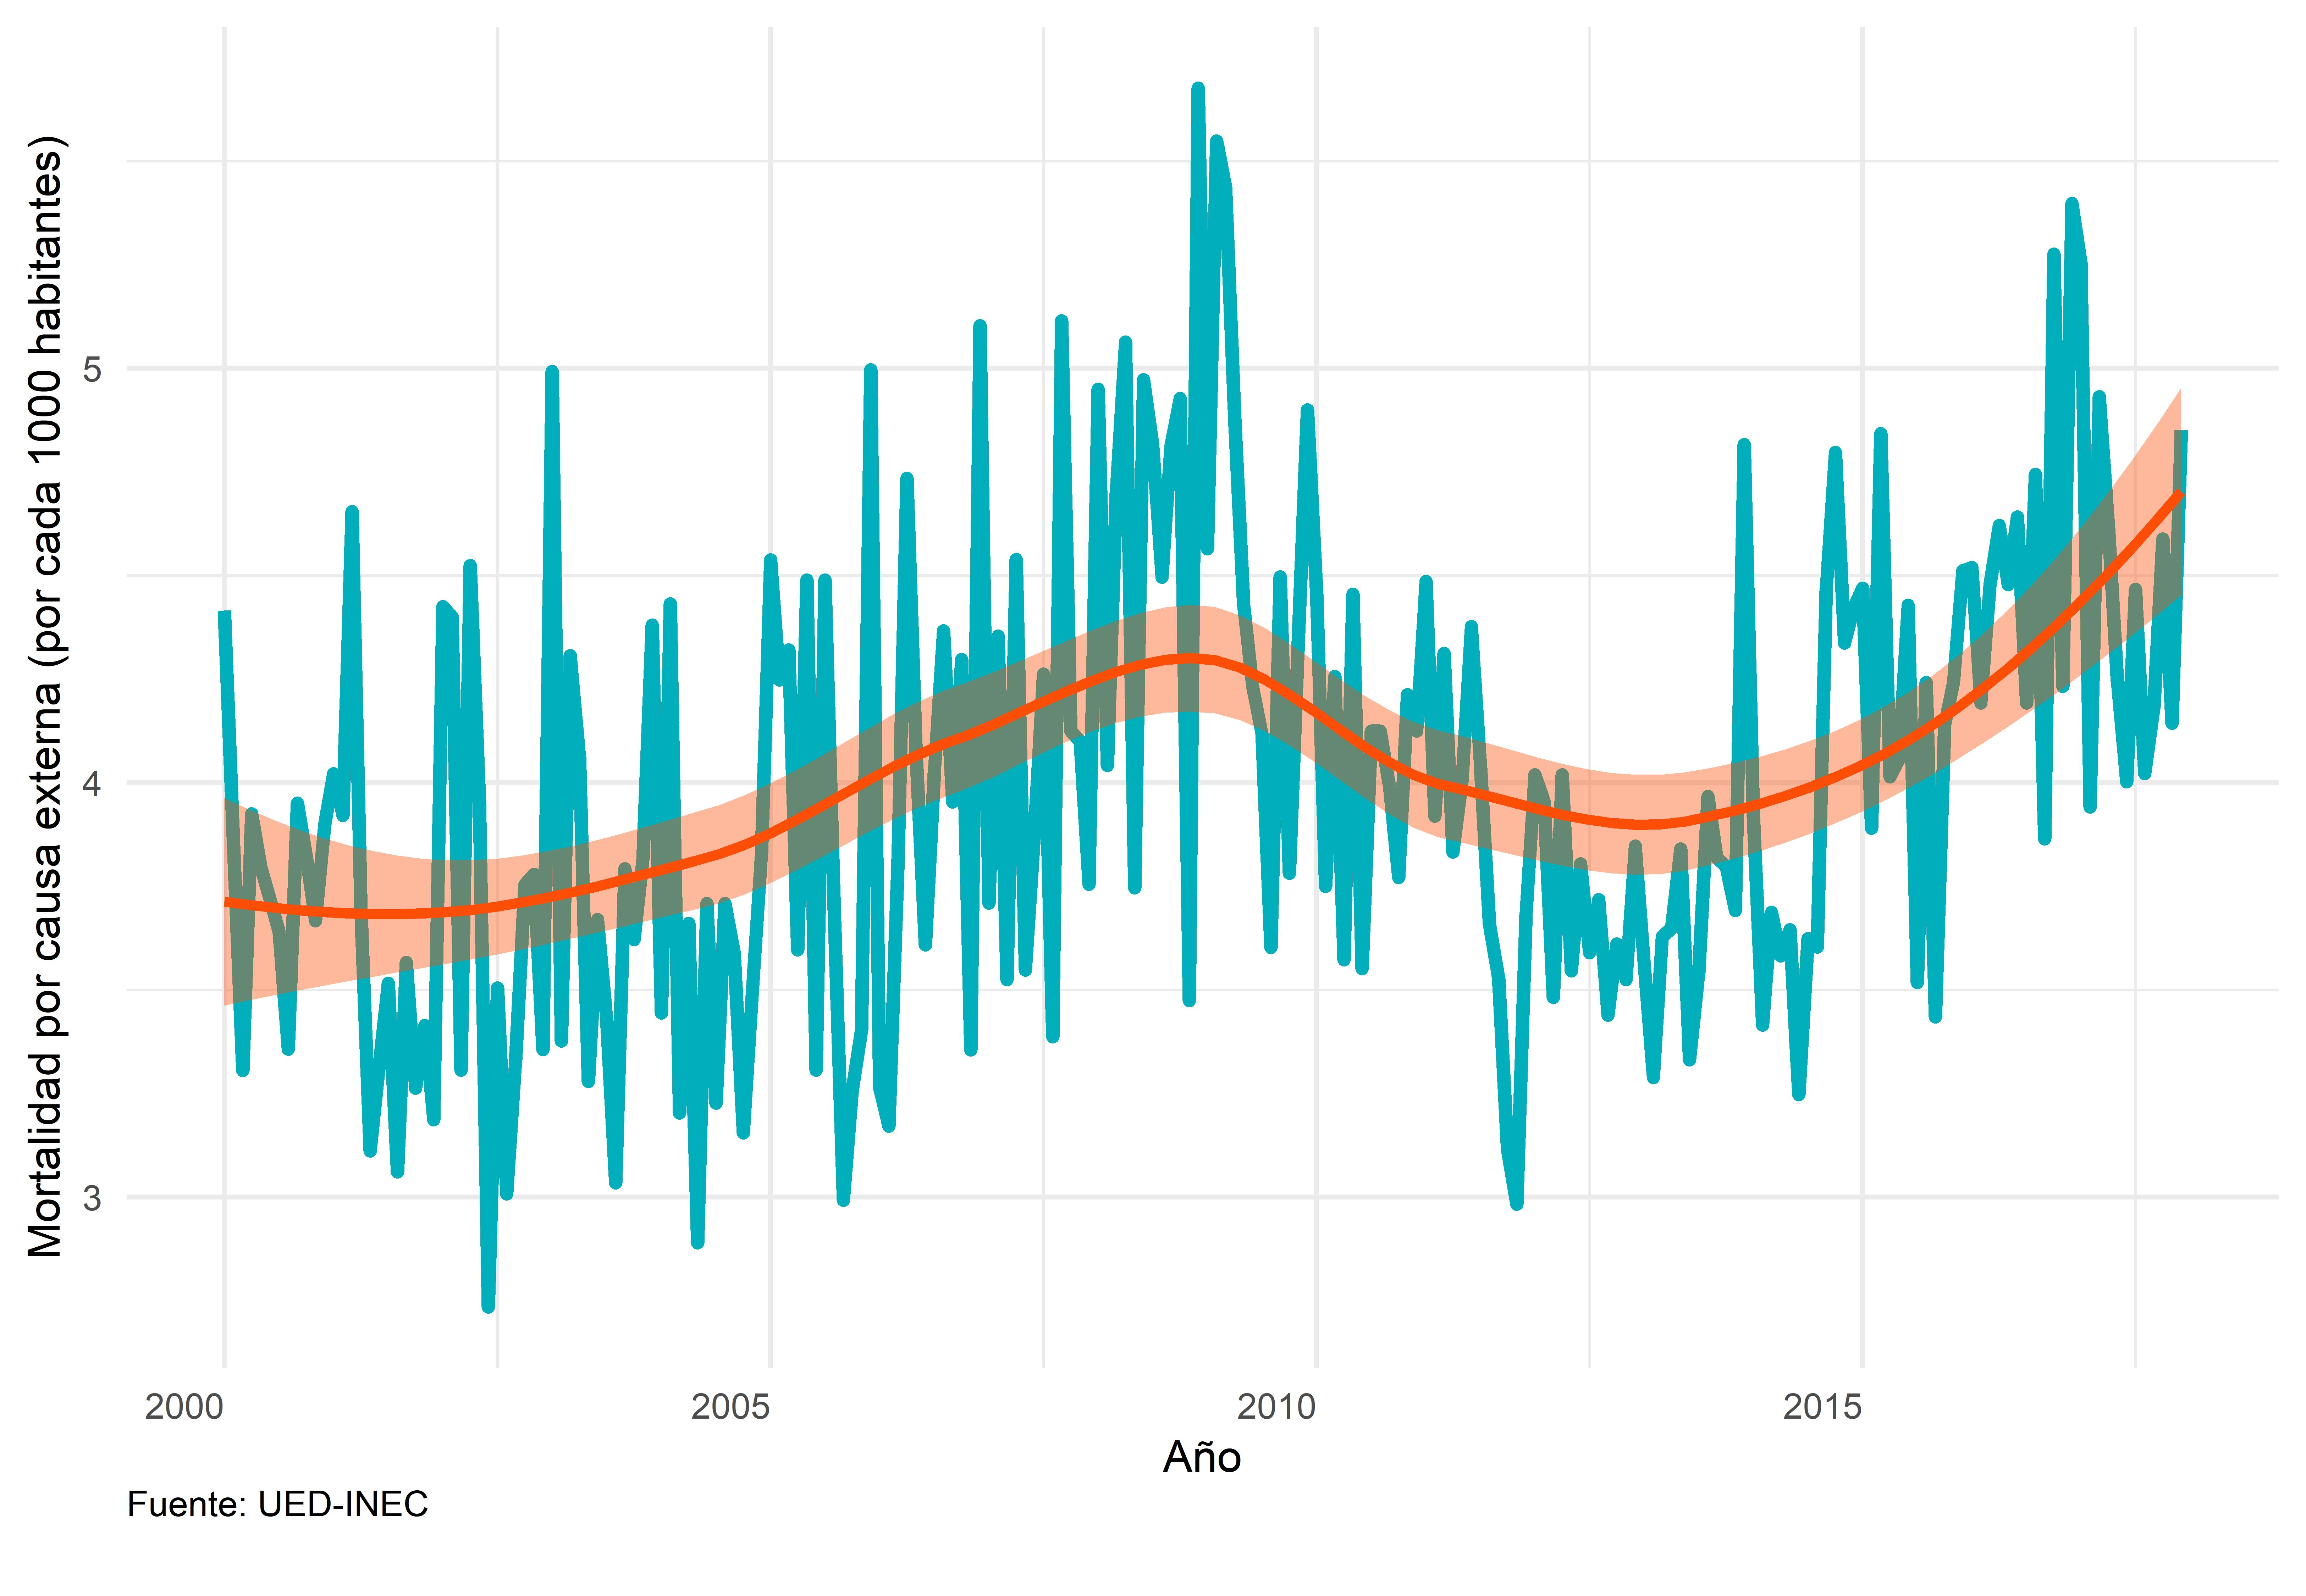
\includegraphics[width=1\linewidth,height=1\textheight]{Tesis_files/figure-latex/externaplotgeneral-1} \caption{Mortalidad por causa externa 2000 - 2017}\label{fig:externaplotgeneral}
\end{figure}

Es importante recalcar que, entre Junio del año 2012 y Diciembre del año
2017, el aumento en la tasa de cambio de la cantidad de defunciones
debido a causas externas coincide con el aumento de la flotilla de
motocicletas, pues en un período de cinco años esta cifra creció en un
189\% (\protect\hyperlink{ref-motos}{Vázquez, 2017}). Conviene entonces
verificar el comportamiento a lo interno de la serie en referencias a
las categorías de las causas externas.

De la figura \ref{fig:externasplotperiodos} puede notarse que cada mes
tiene sus picos y valles durante cada mes a lo largo del periodo, siendo
los meses de Enero, Abril y Diciembre los que presentaron valores
ligeramente más altos entre los años 2000 y 2017.

\begin{figure}[!h]
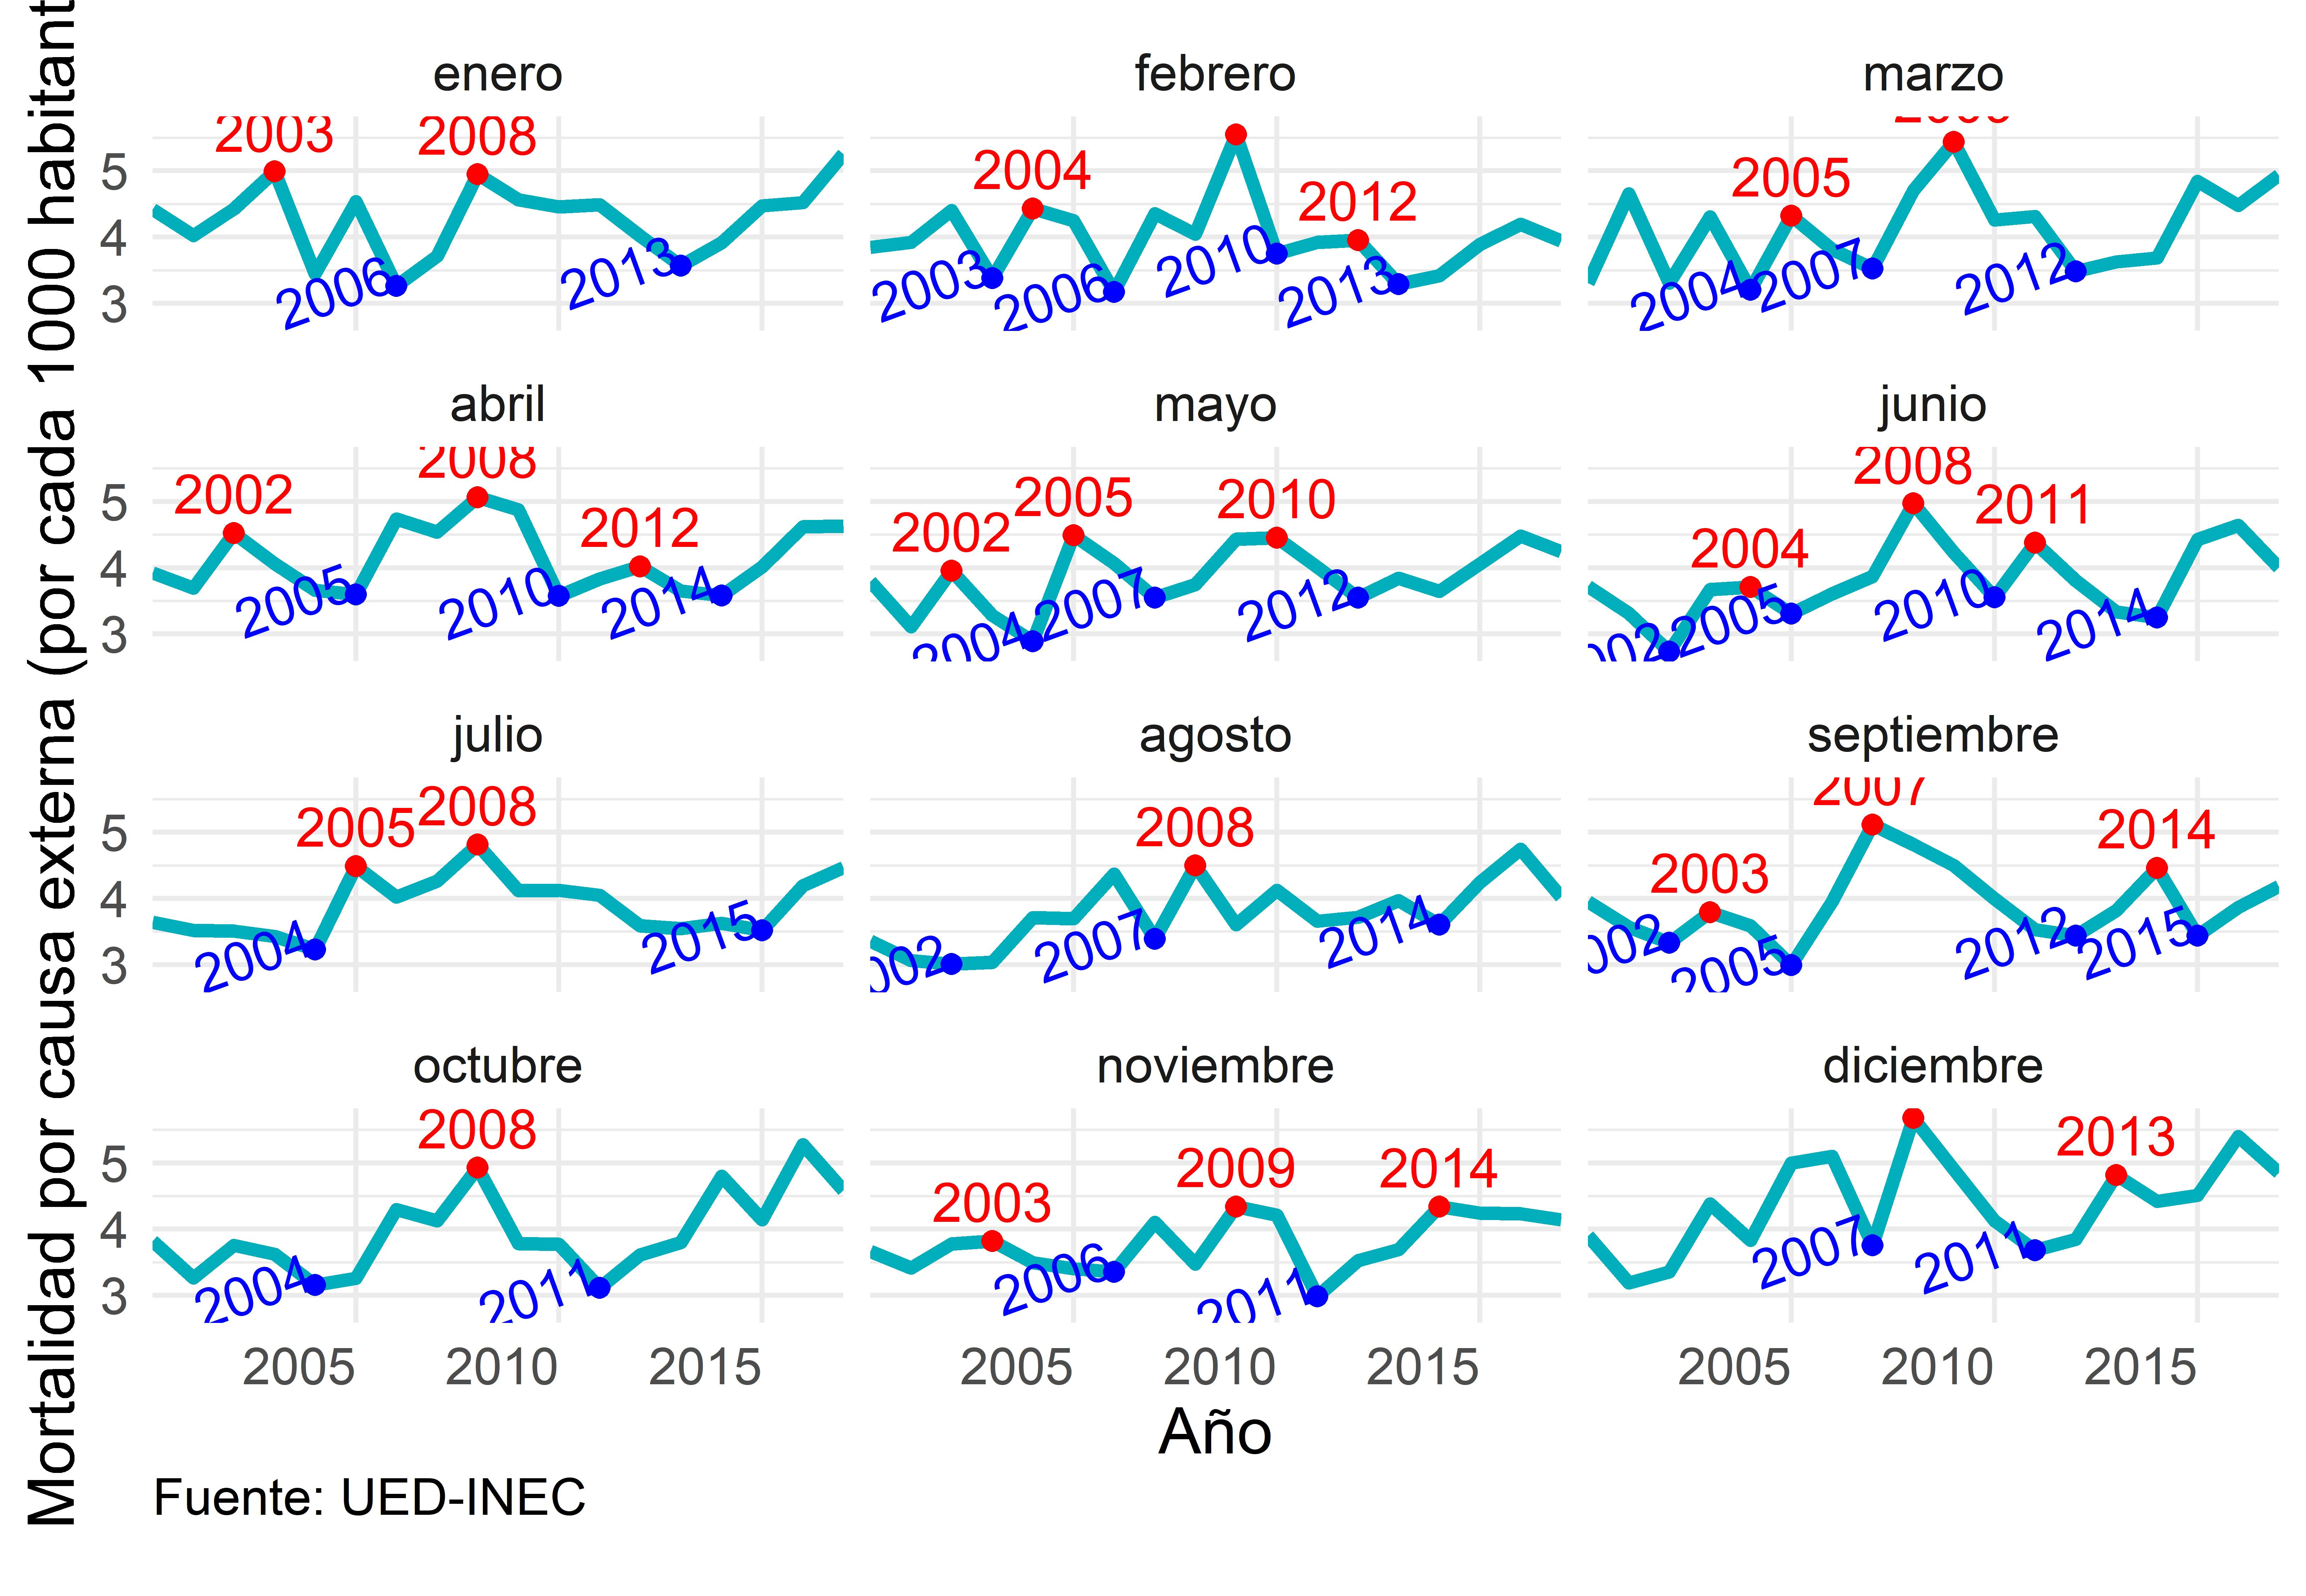
\includegraphics[width=1\linewidth,height=1\textheight]{Tesis_files/figure-latex/externasplotperiodos-1} \caption{Mortalidad por causa externa 2000 - 2017 según mes}\label{fig:externasplotperiodos}
\end{figure}

La descomposición de la serie se hará de forma aditiva debido a que en
el gráfico 1 no se observan grandes cambios en la variabilidad a lo
largo del tiempo. La figura \ref{fig:externasplotdescomposicion} muestra
que la tendencia se mantiene casi constante a lo largo del tiempo,
mientras que parece haber estacionalidad en ciertos lapsos de la segunda
mitad del año. Además, el componente aleatorio muestra como los errores
no son constantes a lo largo de todo el período.

\begin{figure}[!h]
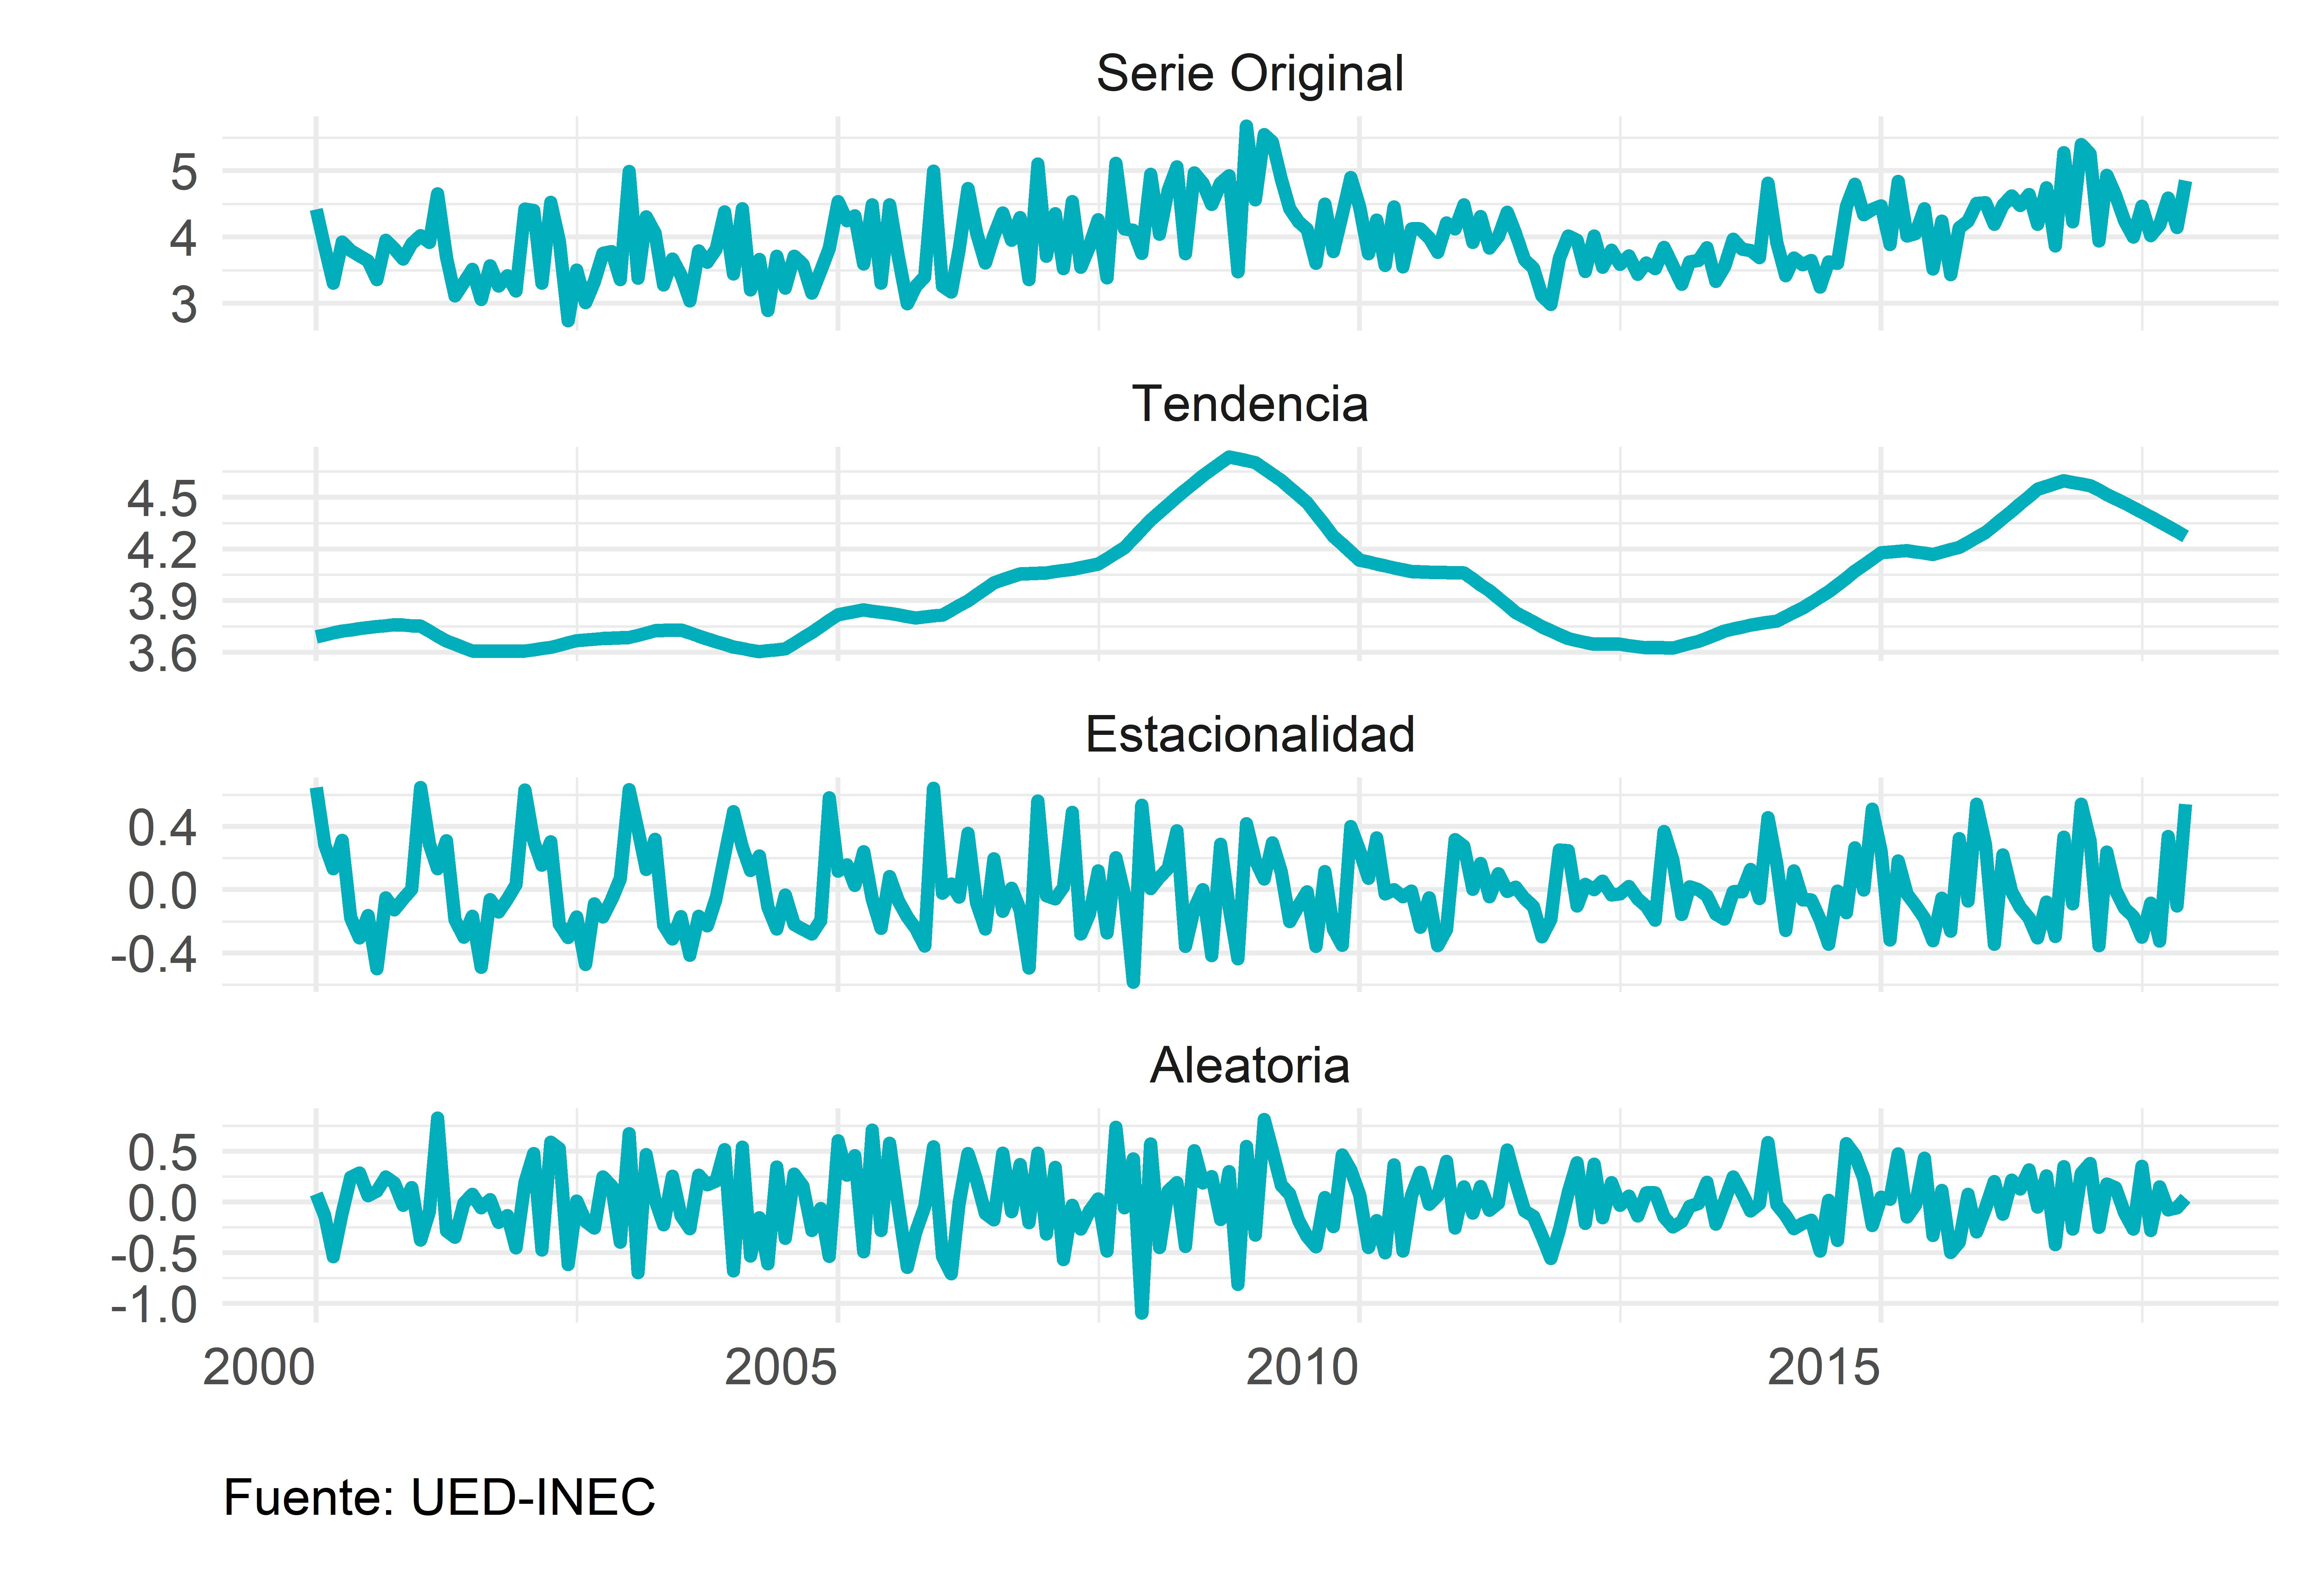
\includegraphics[width=1\linewidth,height=1\textheight]{Tesis_files/figure-latex/externasplotdescomposicion-1} \caption{Descomposición de las defunciones por causa externa en el periodo 2000-2017}\label{fig:externasplotdescomposicion}
\end{figure}

De manera similar a lo hecho para pronosticar la TMII, se ajusta un
modelo utilizando la función \texttt{auto.arima()}, siendo el modelo
sugerido un \(ARIMA(1,1,1)\); mientras que la sobreparametrización
propone como mejor modelo un \(ARIMA(2,0,1)(0,1,1)_{12}\). El cuadro
\ref{tab:externasmedidas} muestra las medidas de rendimiento obtenidas
de los pronósticos realizados con cada método, los cuáles son mejores al
utilizar la sobreparametrización; este hecho también se observa
gráficamente mediante la figura \ref{fig:externasplotpronostico}

\begin{table}[!h]

\caption{\label{tab:unnamed-chunk-15}\label{tab:externasmedidas}Medidas de rendimiento según método de estimación para la Mortalidad por causa externa}
\centering
\resizebox{\linewidth}{!}{
\begin{tabu} to \linewidth {>{\raggedleft}X>{\raggedleft}X>{\raggedleft}X>{\raggedleft}X}
\toprule
Método & RMSE & MAE & MAPE\\
\midrule
autoarima & 0.7555003 & 0.6508858 & 14.35132\\
sobreparametrizacion & 0.7058923 & 0.6011625 & 13.27879\\
\bottomrule
\end{tabu}}
\end{table}

\begin{figure}[!h]
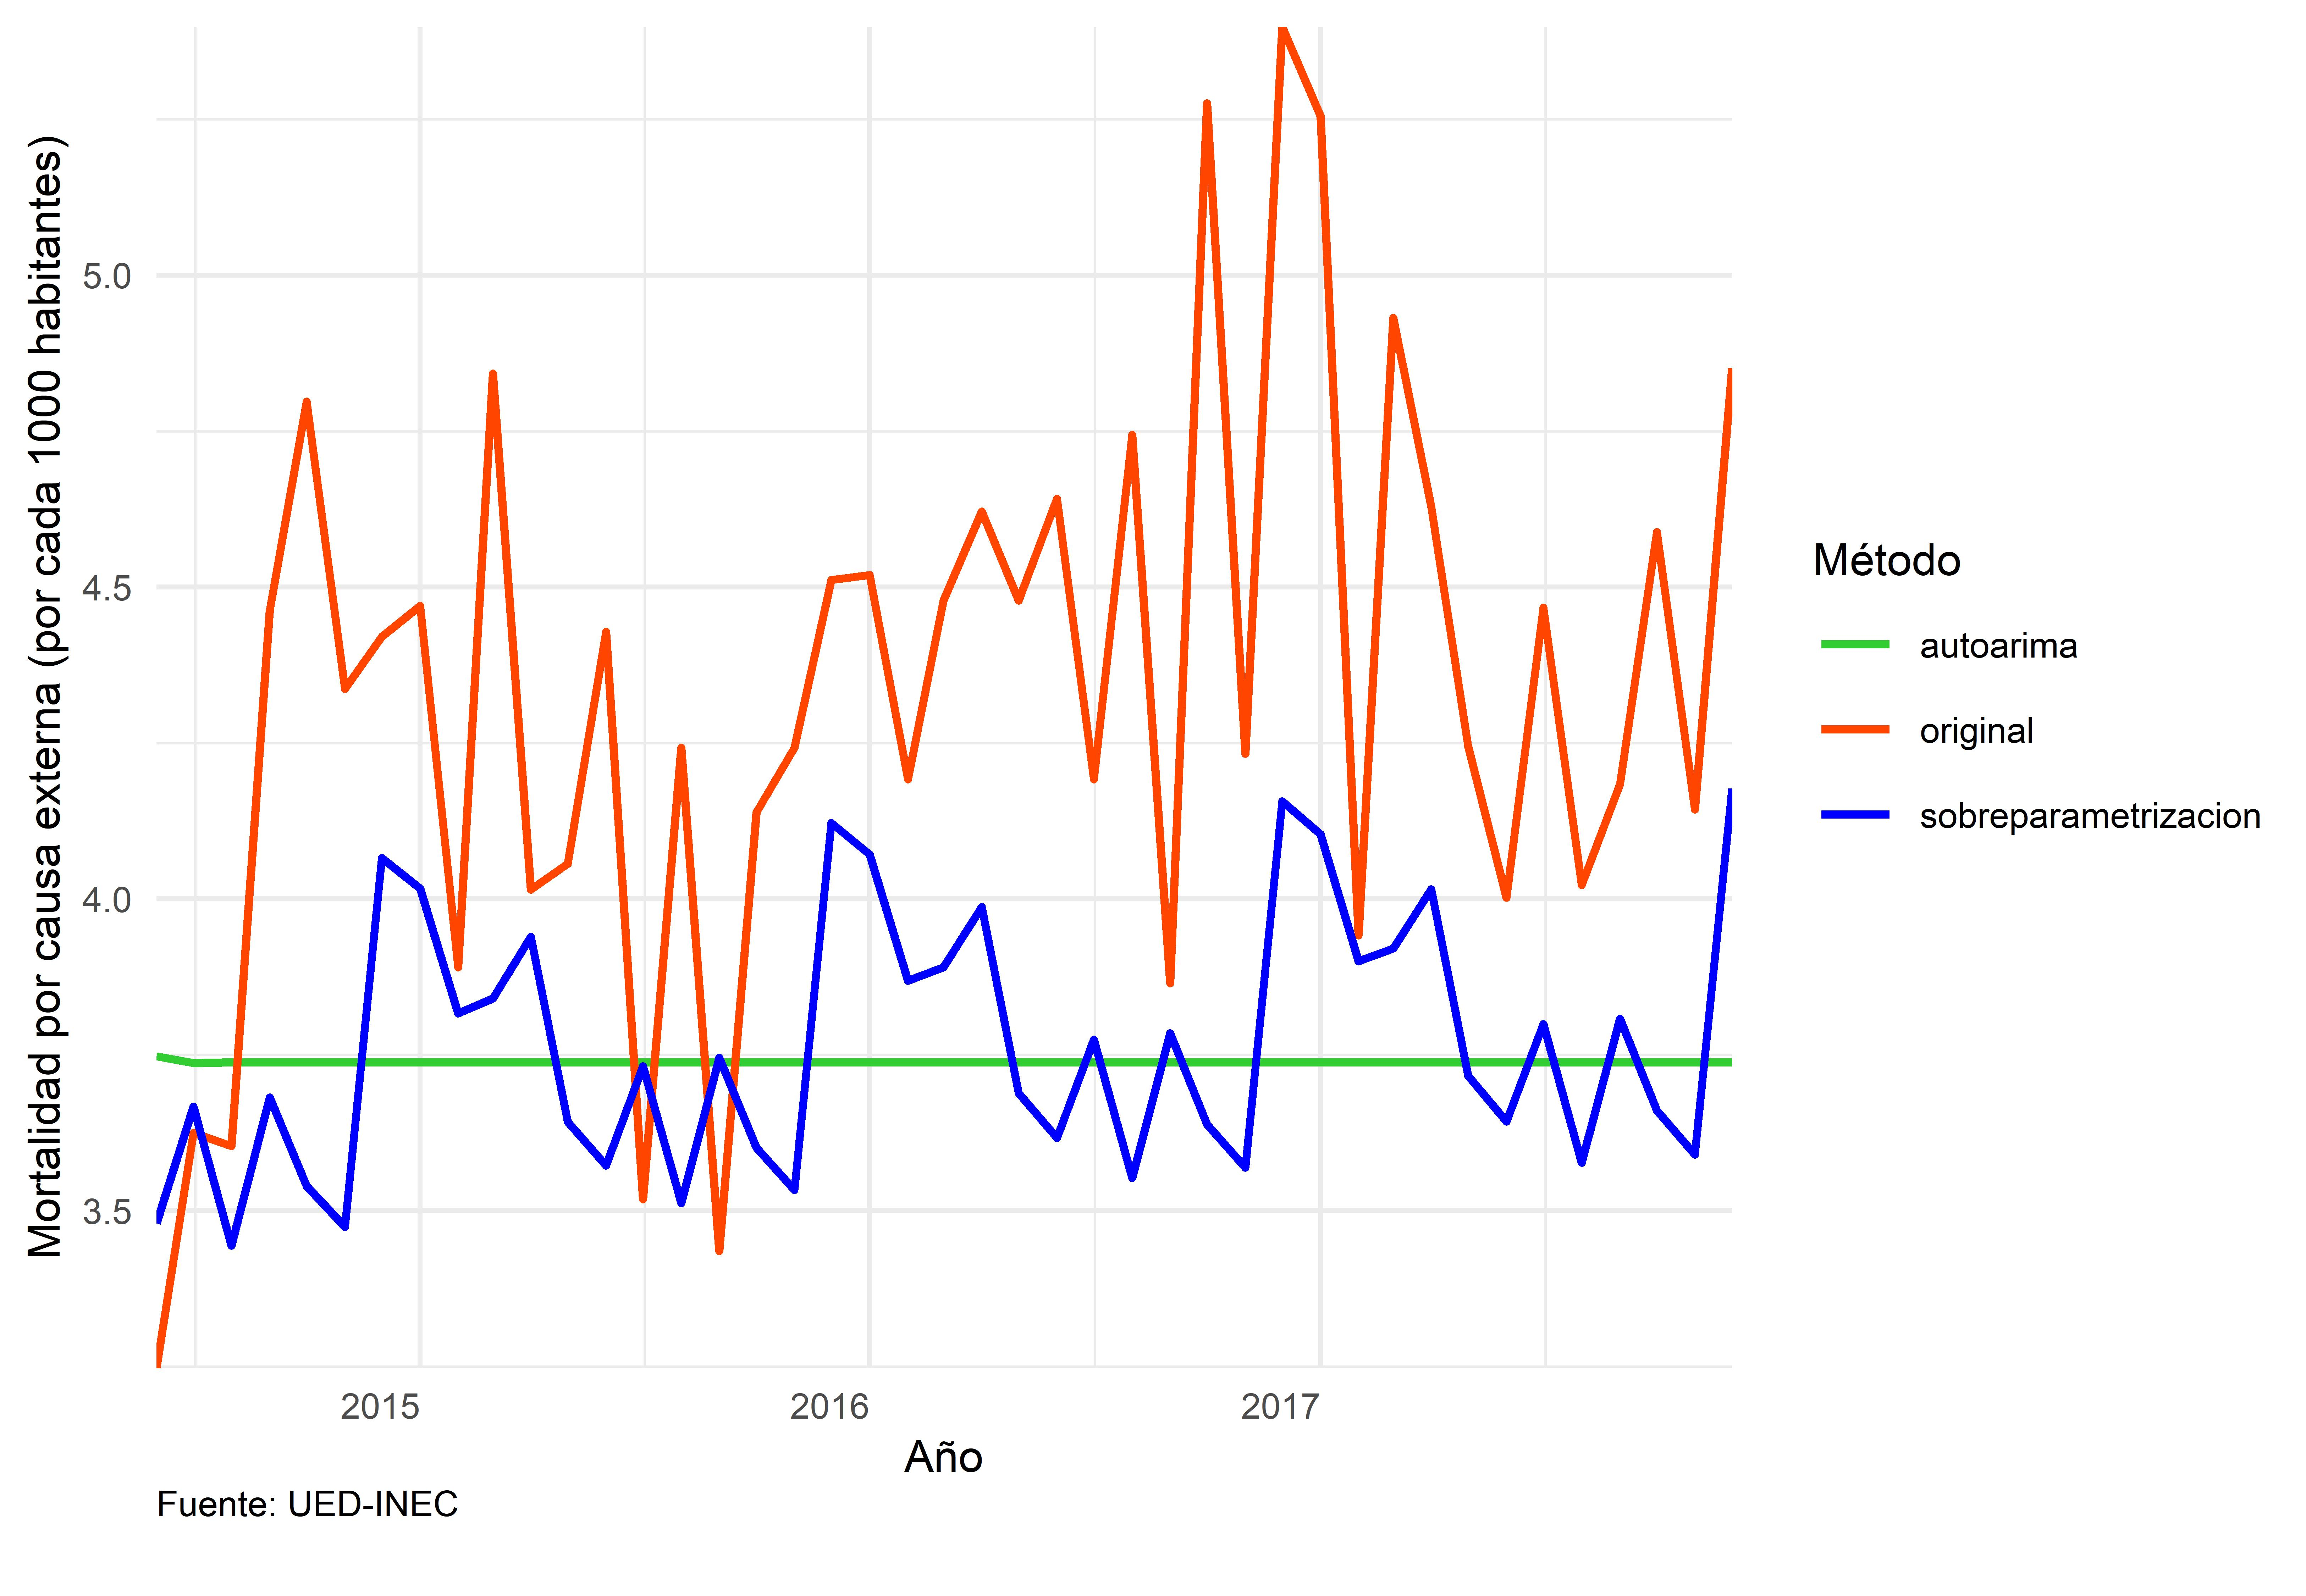
\includegraphics[width=1\linewidth,height=1\textheight]{Tesis_files/figure-latex/externasplotpronostico-1} \caption{Pronósticos de la TMII según método de estimación}\label{fig:externasplotpronostico}
\end{figure}

\subsubsection{Incentivos salariales del sector público}

Los incentivos salariales son retribuciones que de conformidad con la
legislación vigente se asignan al servidor por sus características
laborales que complementan las remuneraciones básicas. Los incentivos se
reconocen tanto a profesionales como a no profesionales, facultados por
disposiciones jurídicas que así lo autorizan. Algunos de estos
incentivos son: anualidades, dedicación exclusiva, salario escolar,
carrera profesional, carrera técnica, zonaje, desarraigo,
regionalización, riesgo policial, riesgo penitenciario, riesgo de
seguridad y vigilancia, peligrosidad, incentivo didáctico, entre otros.
Esta serie cronológica representa los incentivos salariales en millones
de colones del sector público de Costa Rica de enero 2007 a junio 2015.

De manera análoga a las secciones anteriores, la figura
\ref{fig:incentivosplotgeneral} muestra el comportamiento general de la
serie cronológica. al hacer un suavizamiento Loess hay un ligero cambio
de concavidad a partir de Julio 2008, lo cual sugiere que a partir de
este momento los incentivos salariales vuelvan a alcanzar valores
similares a los mostrados al inicio de la serie. La figura
\ref{fig:incentivosplotperiodos} muestra cómo hay un crecimiento
sostenido de los incentivos en cada mes a lo largo de todo el periodo.
Sin embargo, este crecimiento se da a una tasa mucho mayor en la época
de fin y principio de año.

\begin{figure}[!h]
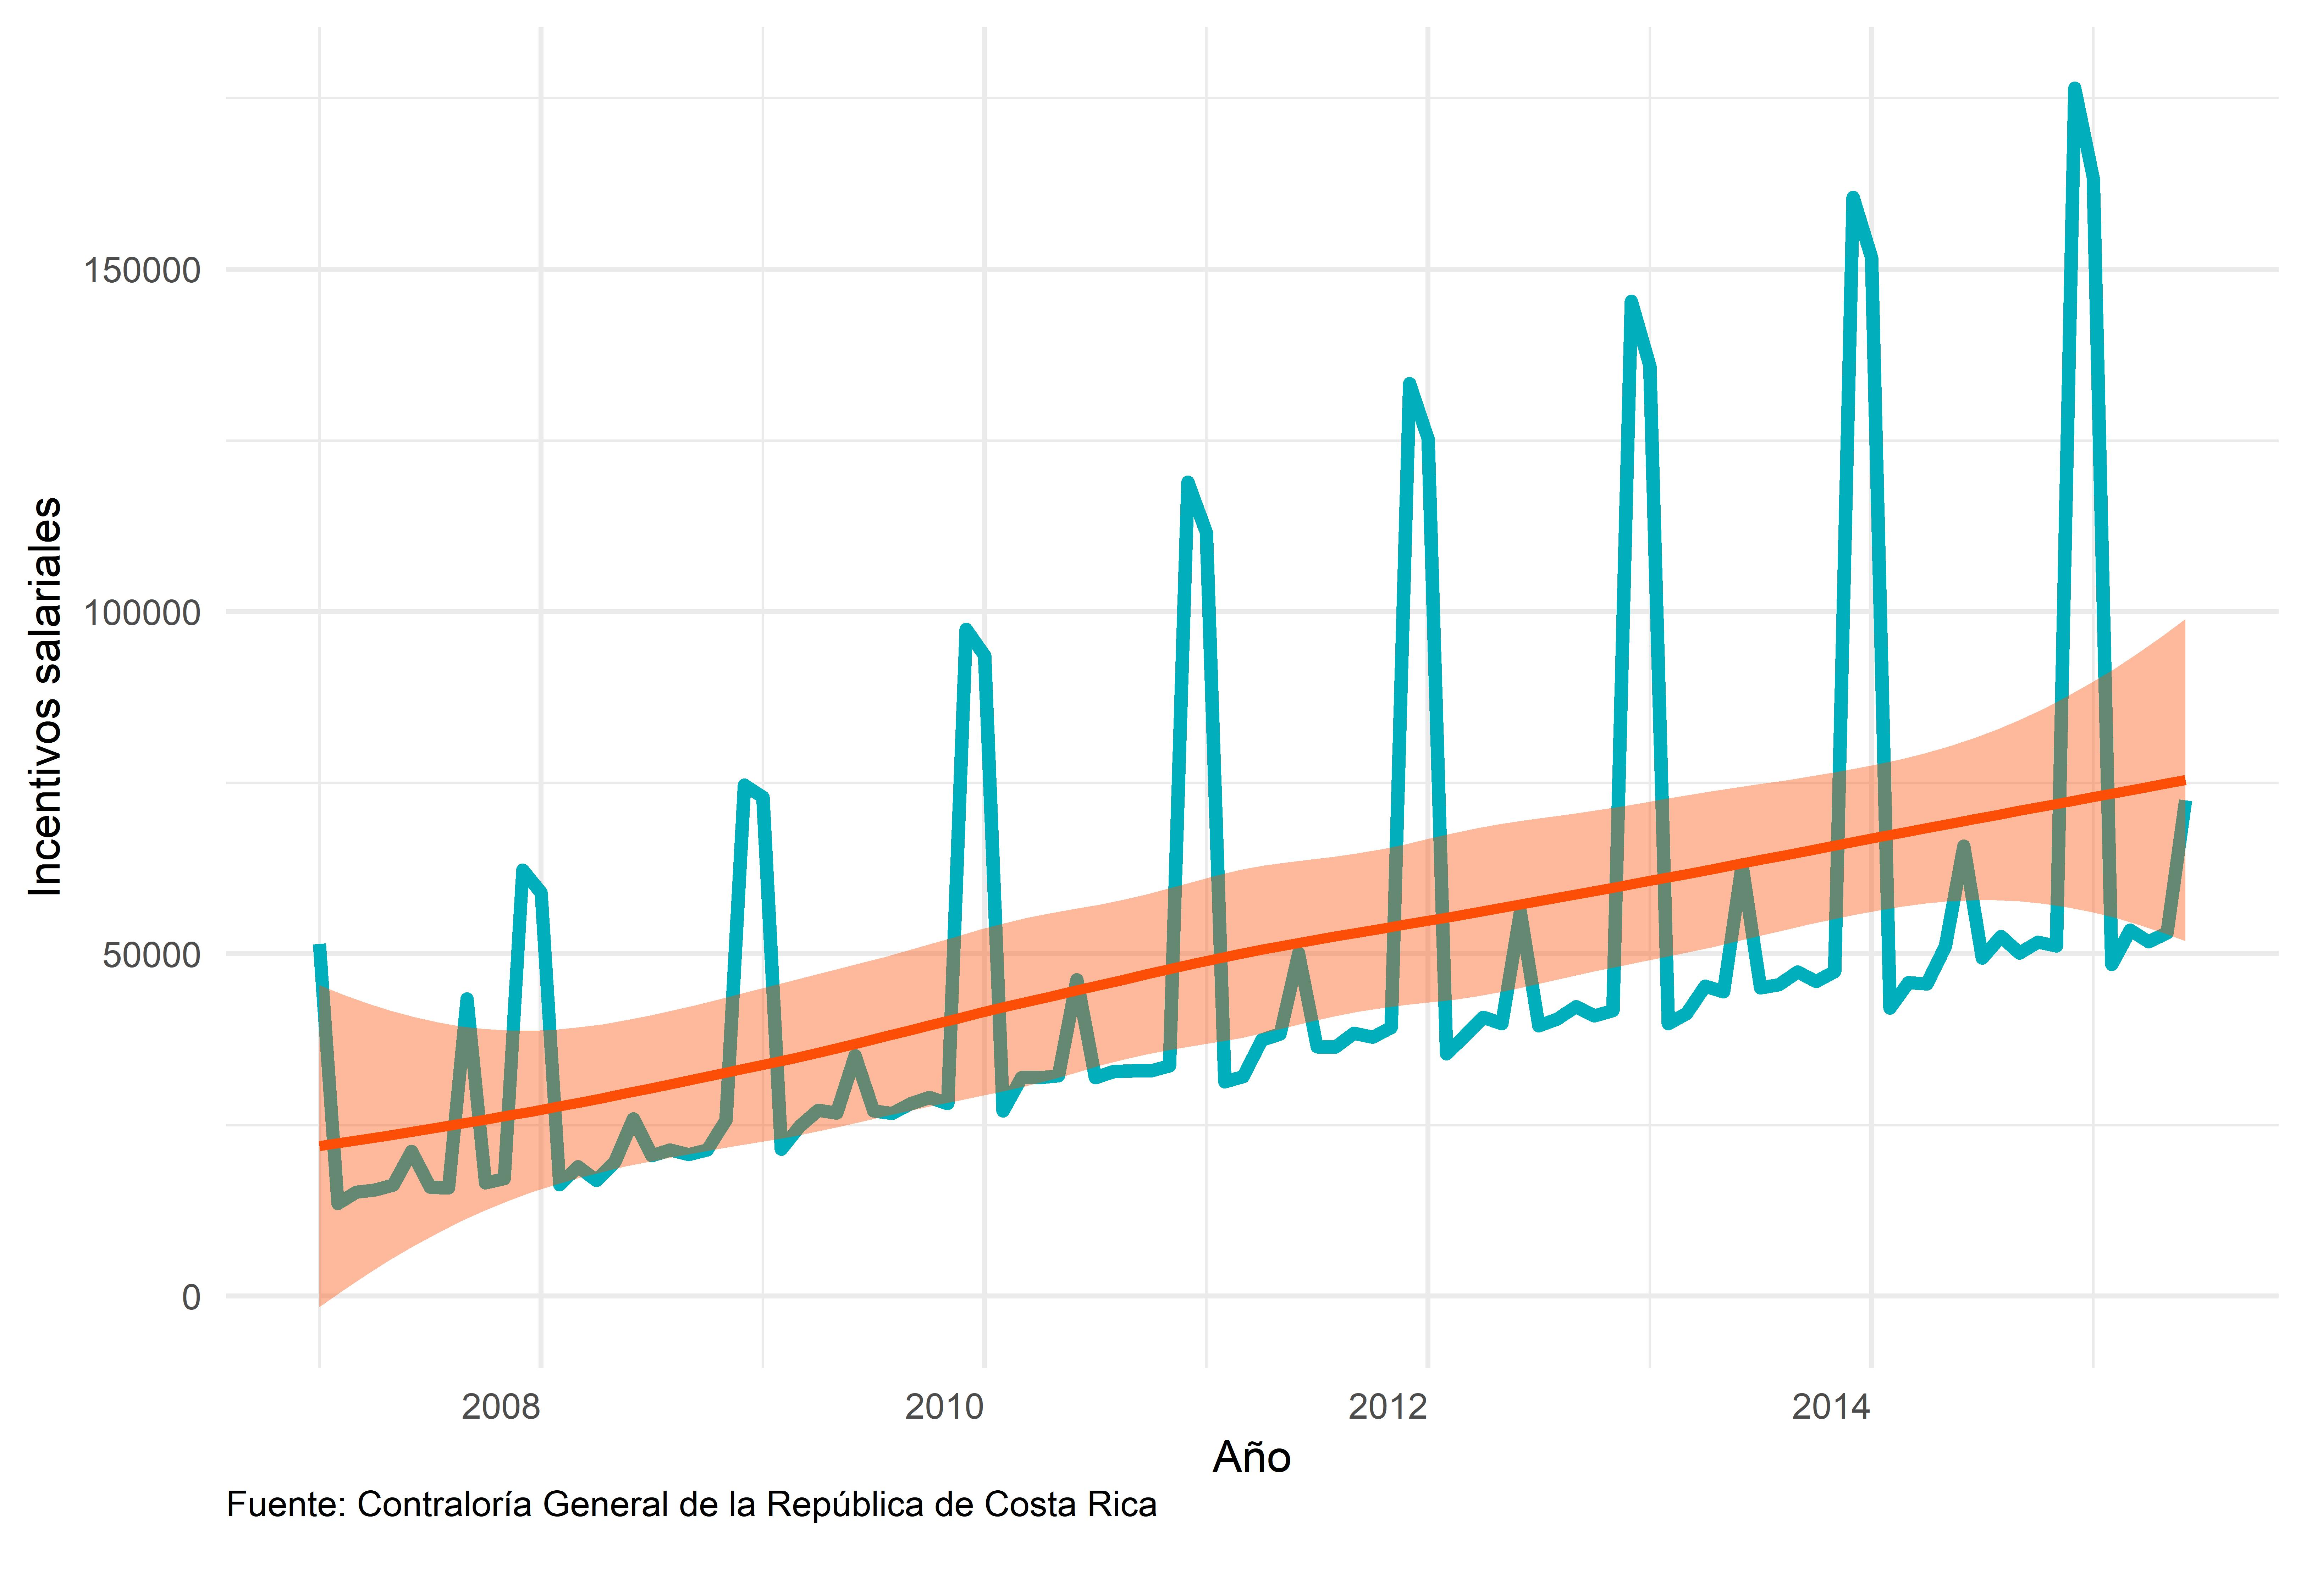
\includegraphics[width=1\linewidth,height=1\textheight]{Tesis_files/figure-latex/incentivosplotgeneral-1} \caption{Incentivos salariales en el sector público 2007 - 2018}\label{fig:incentivosplotgeneral}
\end{figure}

\begin{figure}[!h]
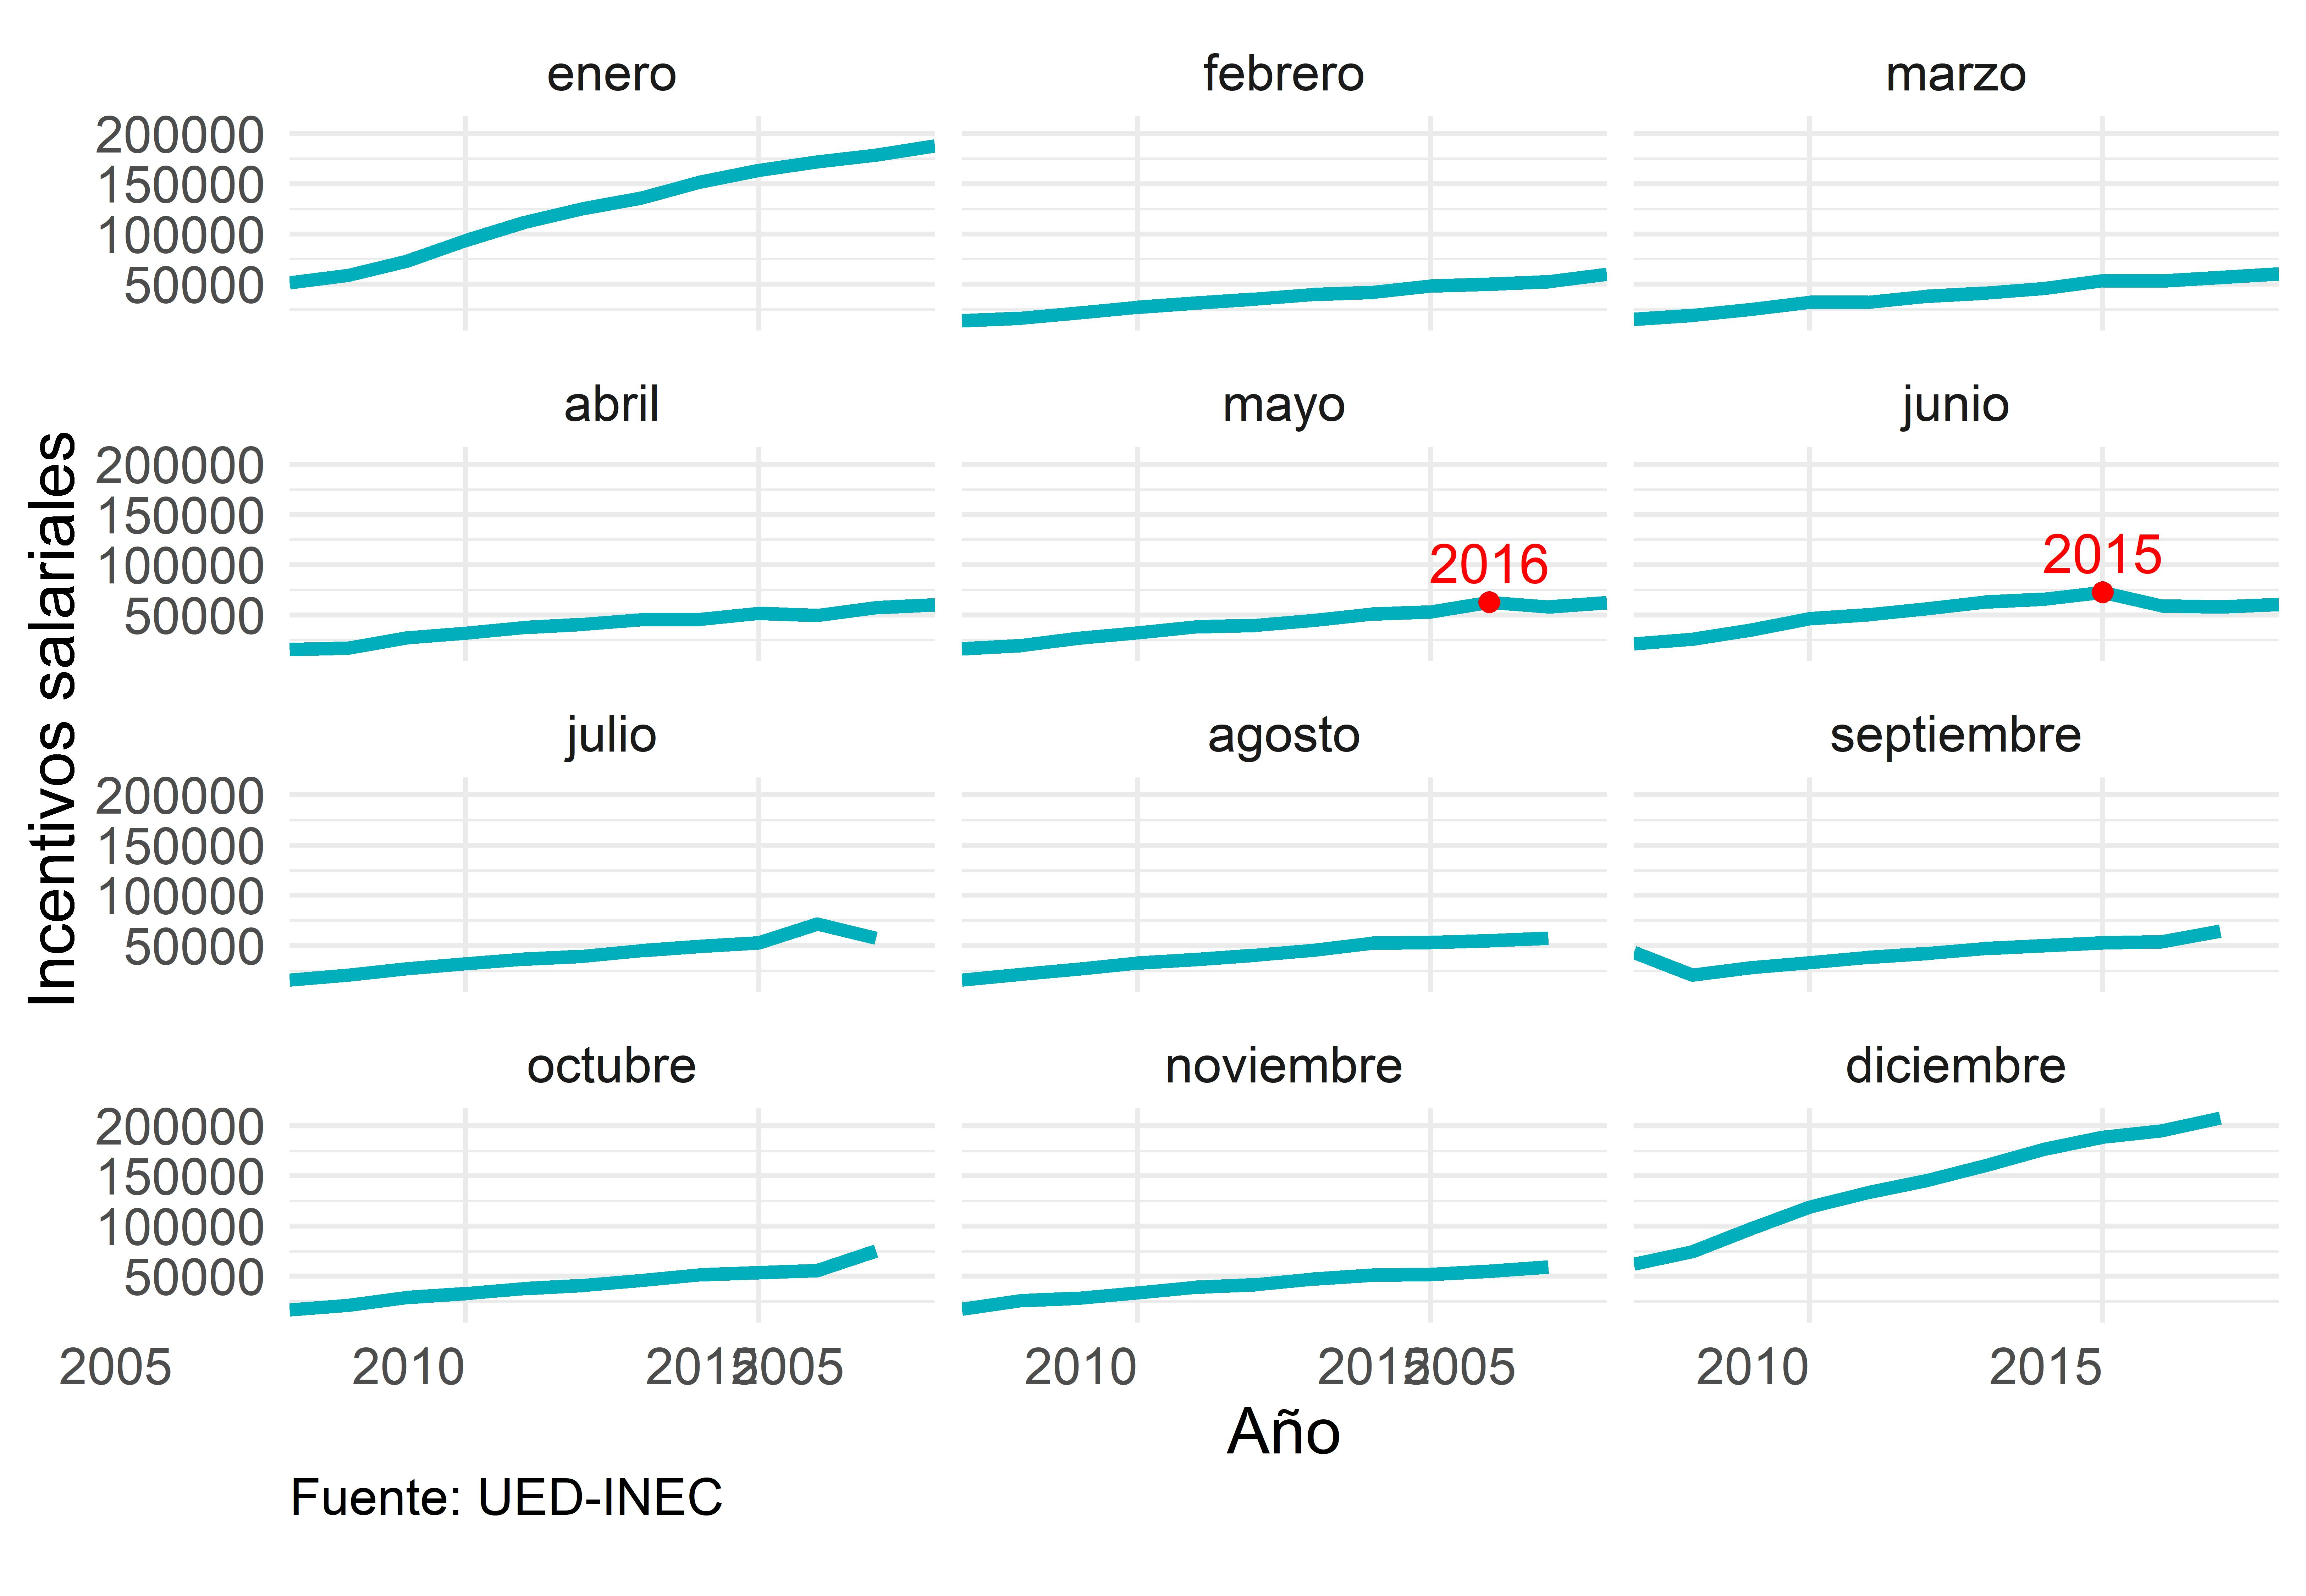
\includegraphics[width=1\linewidth,height=1\textheight]{Tesis_files/figure-latex/incentivosplotperiodos-1} \caption{Incentivos salariales en el sector público 2007 - 2018 según mes}\label{fig:incentivosplotperiodos}
\end{figure}

En la figura \ref{fig:incentivosplotdescomposicion} se muestra la
descomposición de la serie en sus distintos componentes. Pueden
observarse, además de un crecimiento a lo largo del tiempo, los picos y
las caídas en la parte estacional, esto hace referencia a los meses de
Diciembre y Enero; cuando no se está en este periodo los incentivos
poseen un comportamiento más estable. El componente aleatorio muestra
indicios de que la variabilidad de la serie no es homogénea, sino que
cambia conforme pasa el tiempo.

\begin{figure}[!h]
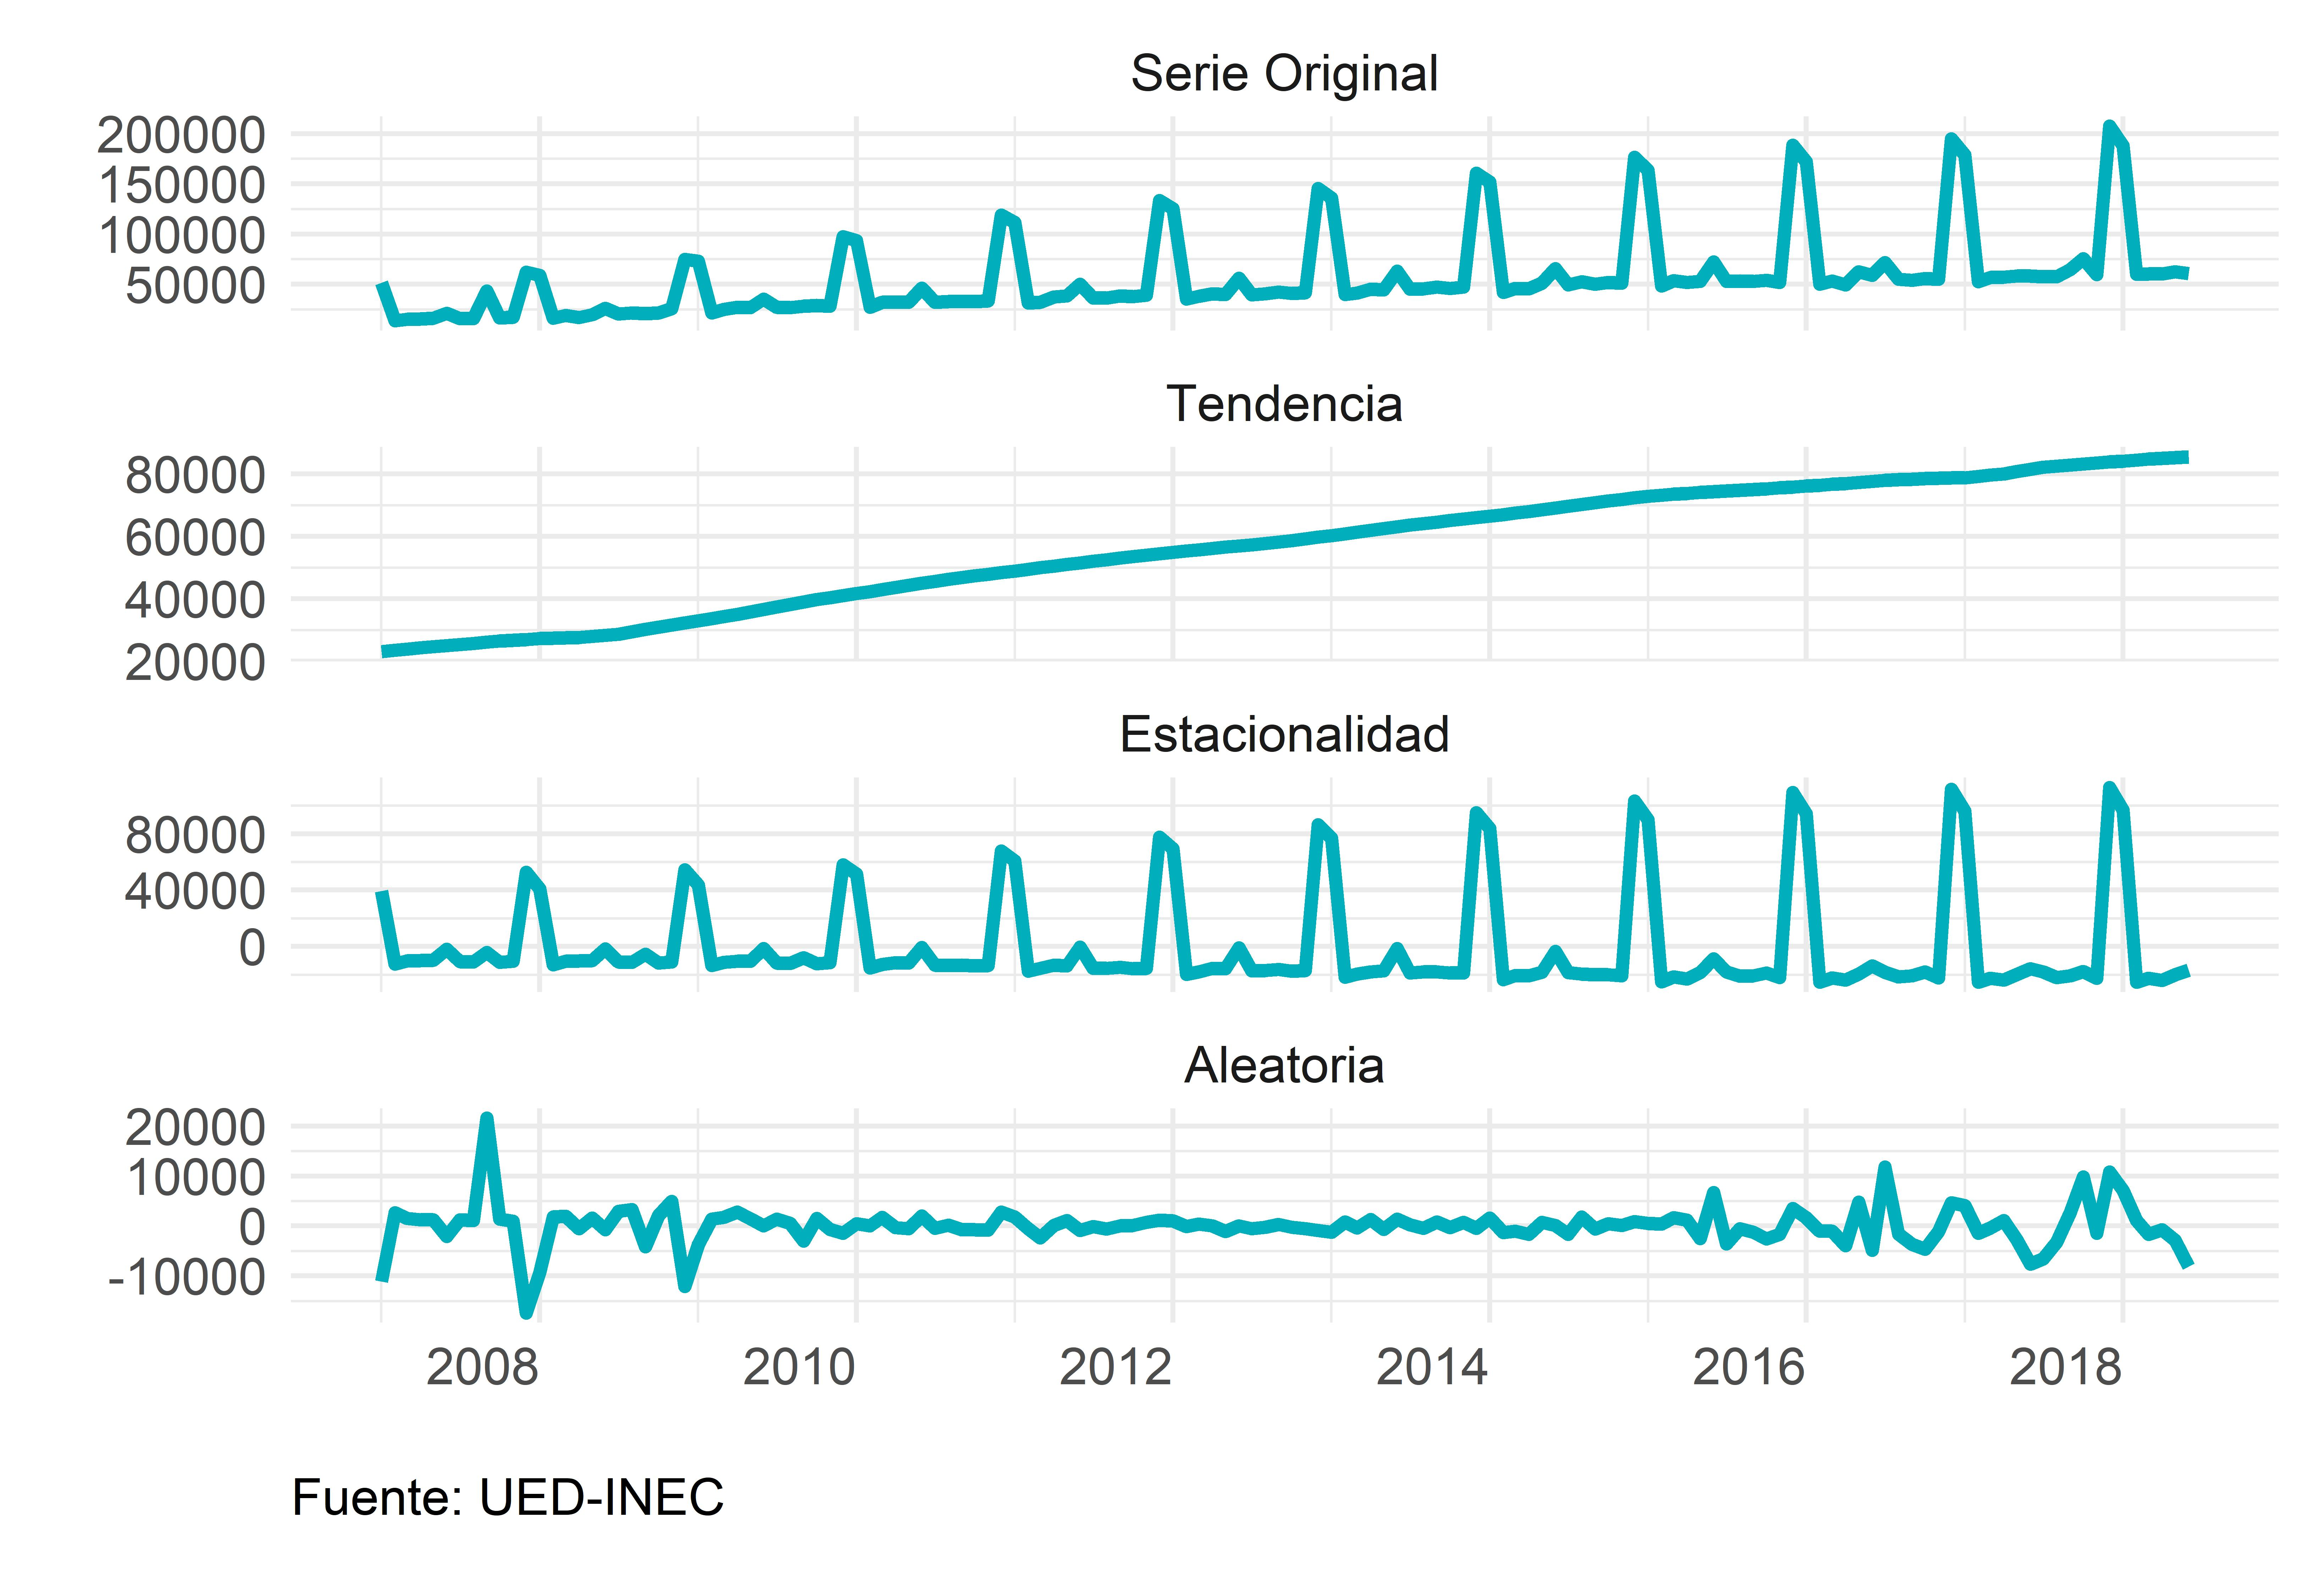
\includegraphics[width=1\linewidth,height=1\textheight]{Tesis_files/figure-latex/incentivosplotdescomposicion-1} \caption{Descomposición de la serie de Incentivos salariales en el periodo 2007 - 2018}\label{fig:incentivosplotdescomposicion}
\end{figure}

Nuevamente, se ajustaron dos modelos ARIMA, el primero de ellos mediante
la función \texttt{auto.arima()}, siendo el modelo sugerido un
\(ARIMA(0,0,1)(1,1,0)_{12}\);y el segudo modelo sugerido, utilizando la
sobreparametrización, es un \(ARIMA(2,1,0)(1,2,0)_{12}\). Tanto el
cuadro \ref{tab:incentivosmedidas} como la figura
\ref{fig:incentivosplotpronostico} muestran que nuevamente los
pronósticos obtenidos son superiores utilizando la sobreparametrización.

\begin{table}[!h]

\caption{\label{tab:unnamed-chunk-17}\label{tab:incentivosmedidas}Medidas de rendimiento según método de estimación para los incentivos salariales}
\centering
\resizebox{\linewidth}{!}{
\begin{tabu} to \linewidth {>{\raggedleft}X>{\raggedleft}X>{\raggedleft}X>{\raggedleft}X}
\toprule
Método & RMSE & MAE & MAPE\\
\midrule
autoarima & 5212.797 & 3701.074 & 4.498137\\
sobreparametrizacion & 3476.907 & 2846.975 & 4.000943\\
\bottomrule
\end{tabu}}
\end{table}

\begin{figure}[!h]
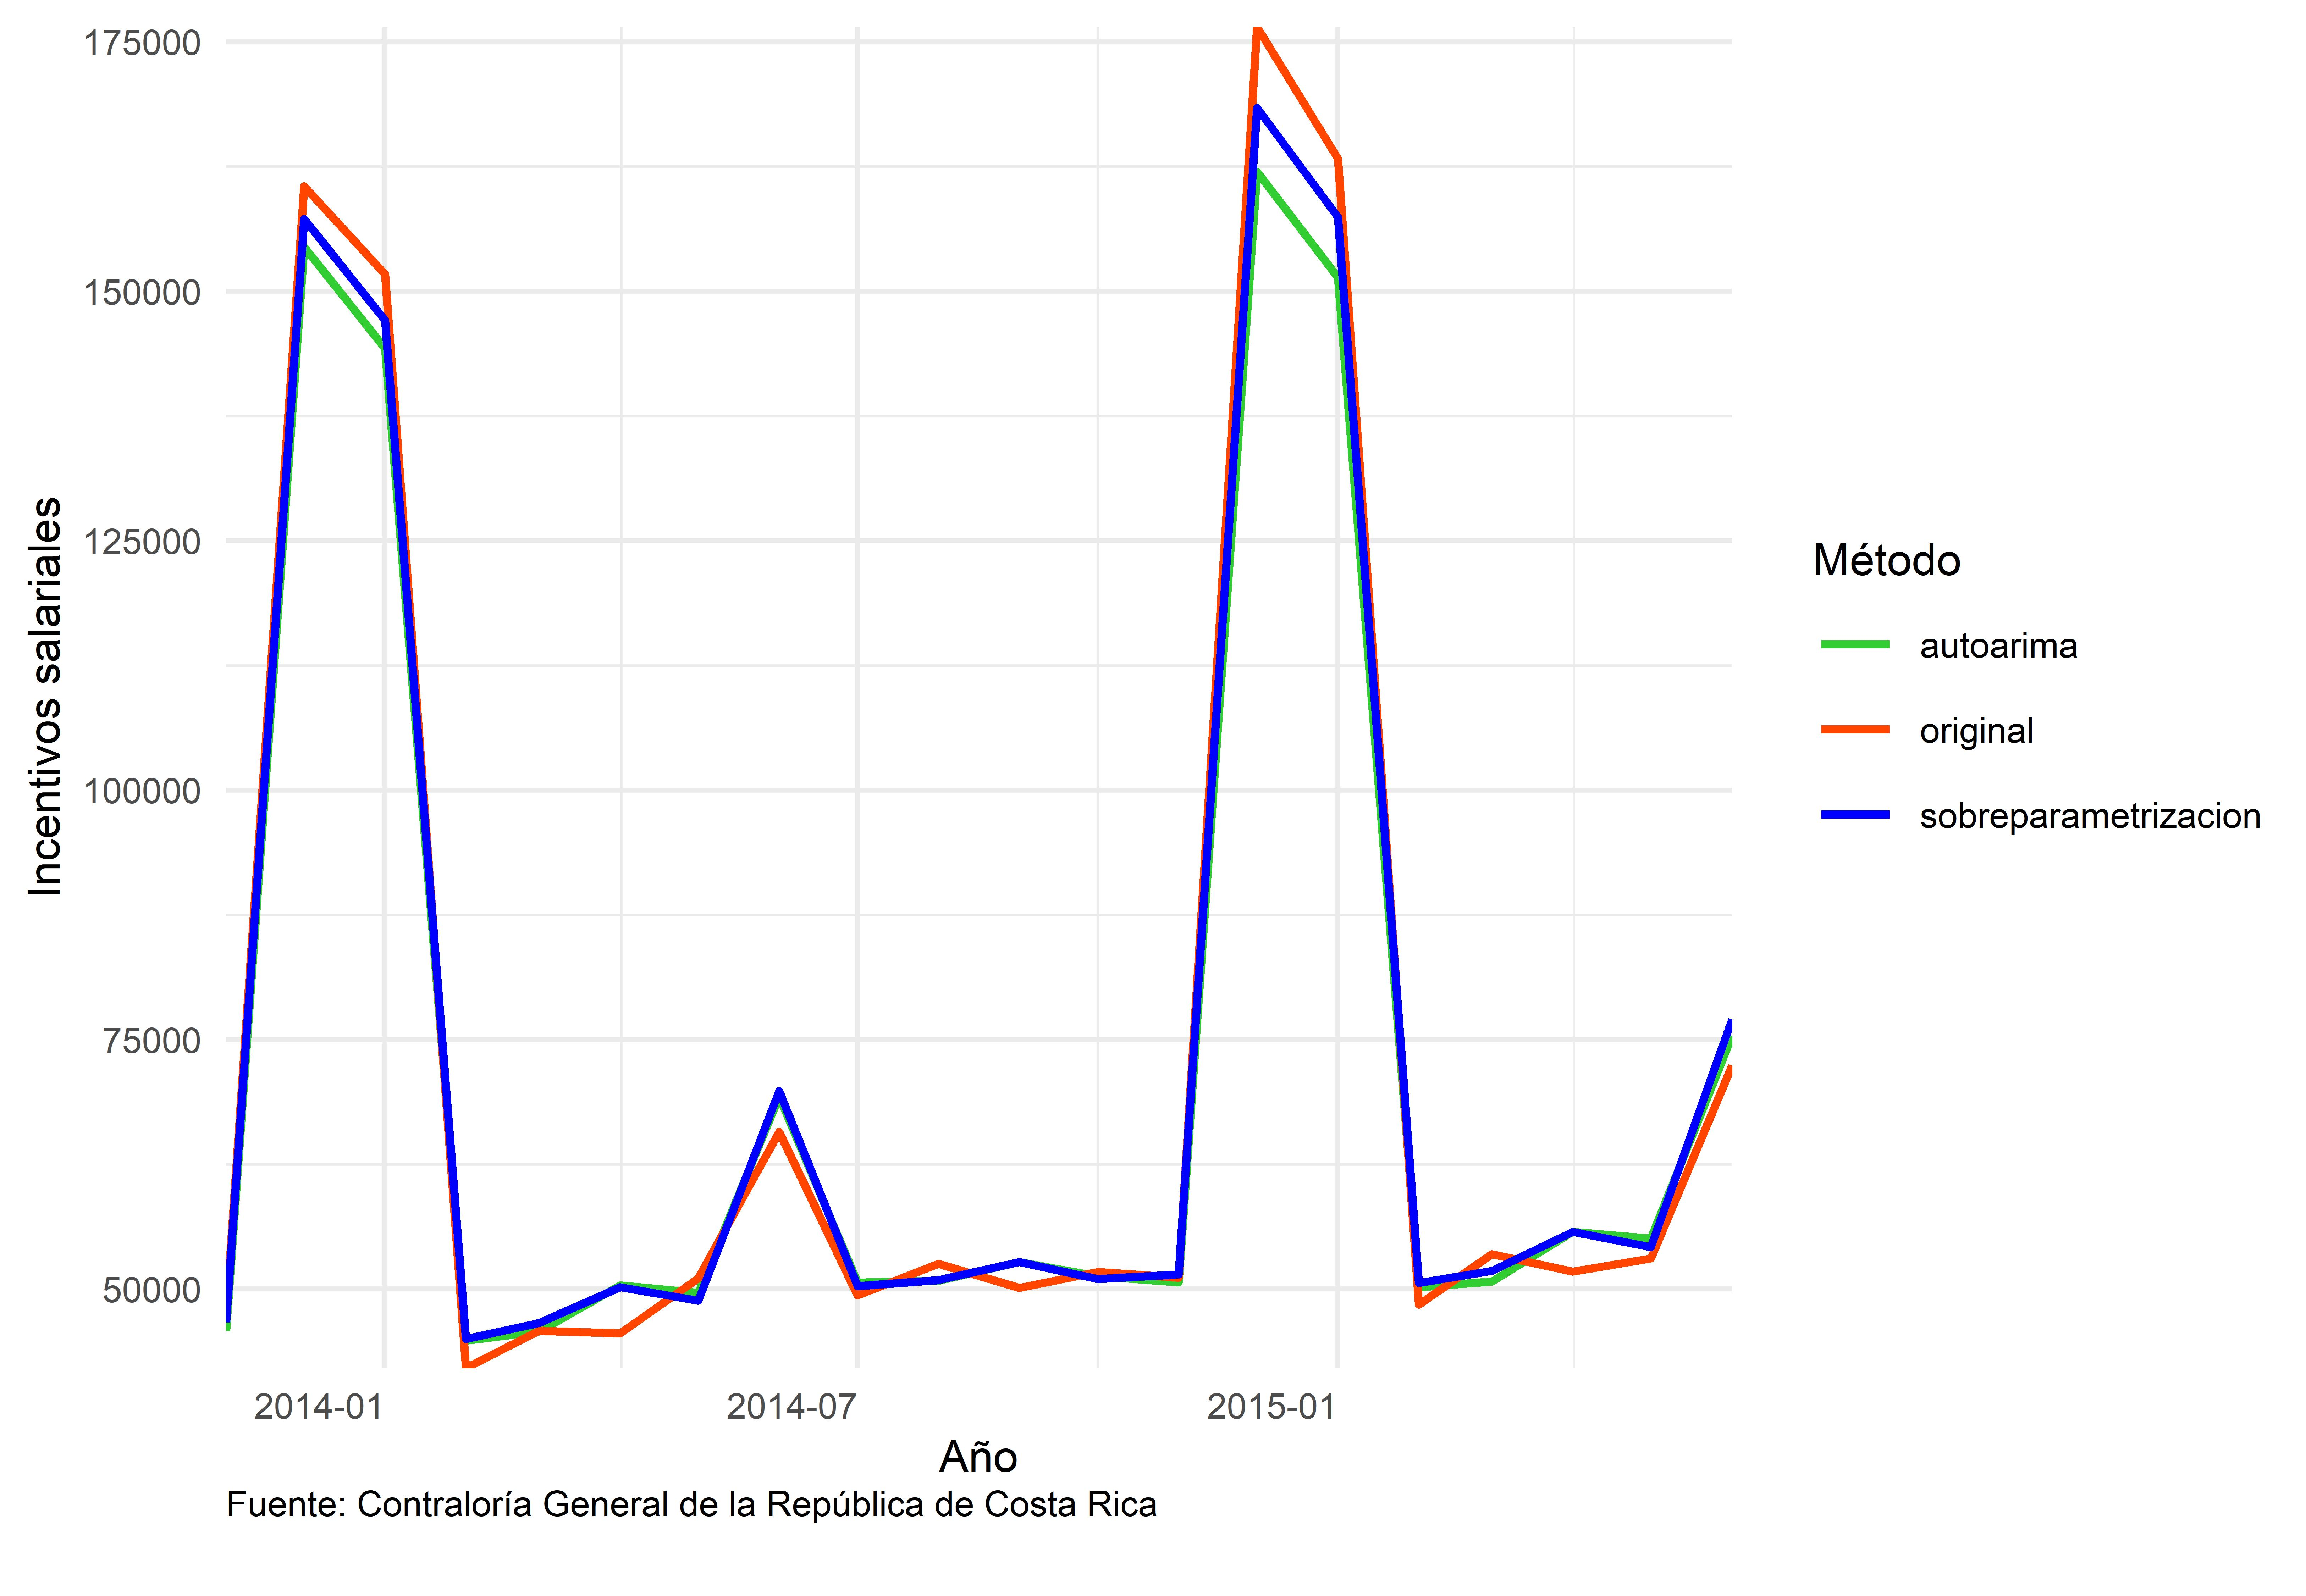
\includegraphics[width=1\linewidth,height=1\textheight]{Tesis_files/figure-latex/incentivosplotpronostico-1} \caption{Pronósticos de los incentivos salariales según método de estimación}\label{fig:incentivosplotpronostico}
\end{figure}

\subsubsection{Intereses y comisiones del sector público}

Finalmente, se utiliza para este análisis la serie cronológica de los
intereses y comisiones del sector público, que comprenden el pago de los
intereses de la deuda del gobierno, esto es, las erogaciones de
intereses y comisiones destinadas por las instituciones públicas para
cubrir el pago a favor de terceras personas, físicas o jurídicas, del
sector privado o del sector público, residentes en el territorio
nacional o en el exterior, por la utilización en un determinado plazo de
recursos financieros provenientes de los conceptos de emisión y
colocación de títulos valores, contratación de préstamos directos,
créditos de proveedores, depósitos a plazo y a la vista, intereses por
deudas de avales asumidos, entre otros pasivos de la entidad tranzados
en el país o en el exterior. Incluye el pago por concepto de otras
obligaciones contraídas entre las partes, que no provienen de las
actividades normales de financiamiento. Además, los intereses y
comisiones por las operaciones normales de los bancos comerciales del
sector público, así como las diferencias por tipo de cambio por
operaciones financieras; y también el pago de intereses moratorios
correspondientes a la deuda pública.

Para iniciar el análisis exploratorio de esta serie, la figura
\ref{fig:interesesplotgeneral} muestra que hay un ligero cambio de
concavidad a partir de Julio 2010, esto sugiere que a partir de este
momento los intereses y comisiones inician una tendencia al alza, la
cual se sostiene hasta Junio del 2018. Por su parte, la figura
\ref{fig:interesesplotperiodos} muestra cómo hay un crecimiento
sostenido de los intereses y comisiones del sector público al final de
cada trimestre durante todo el periodo, mientras que se mantiene casi
constante durante los primeros dos meses de cada trimestre. La caída más
pronunciada se dio en abril del 2015 mientras que la tasa de crecimiento
más rápida parece darse al final del primer trimestre. Además, en la
figura \ref{fig:interesesplotdescomposicion} se muestra la
descomposición de la serie en sus distintos componentes. Puede
observarse, además de un crecimiento a lo largo del tiempo posterior a
una disminución, los picos y las caídas en la parte estacional, esto en
cuanto a los cierres trimestrales previamente mencionados. El componente
aleatorio muestra indicios de que la variabilidad de la serie no es
homogénea, sino que cambia conforme pasa el tiempo, pues durante un
tiempo se mantuvo relativamente estable pero luego presenta algunos
cambios.

\begin{figure}[!h]
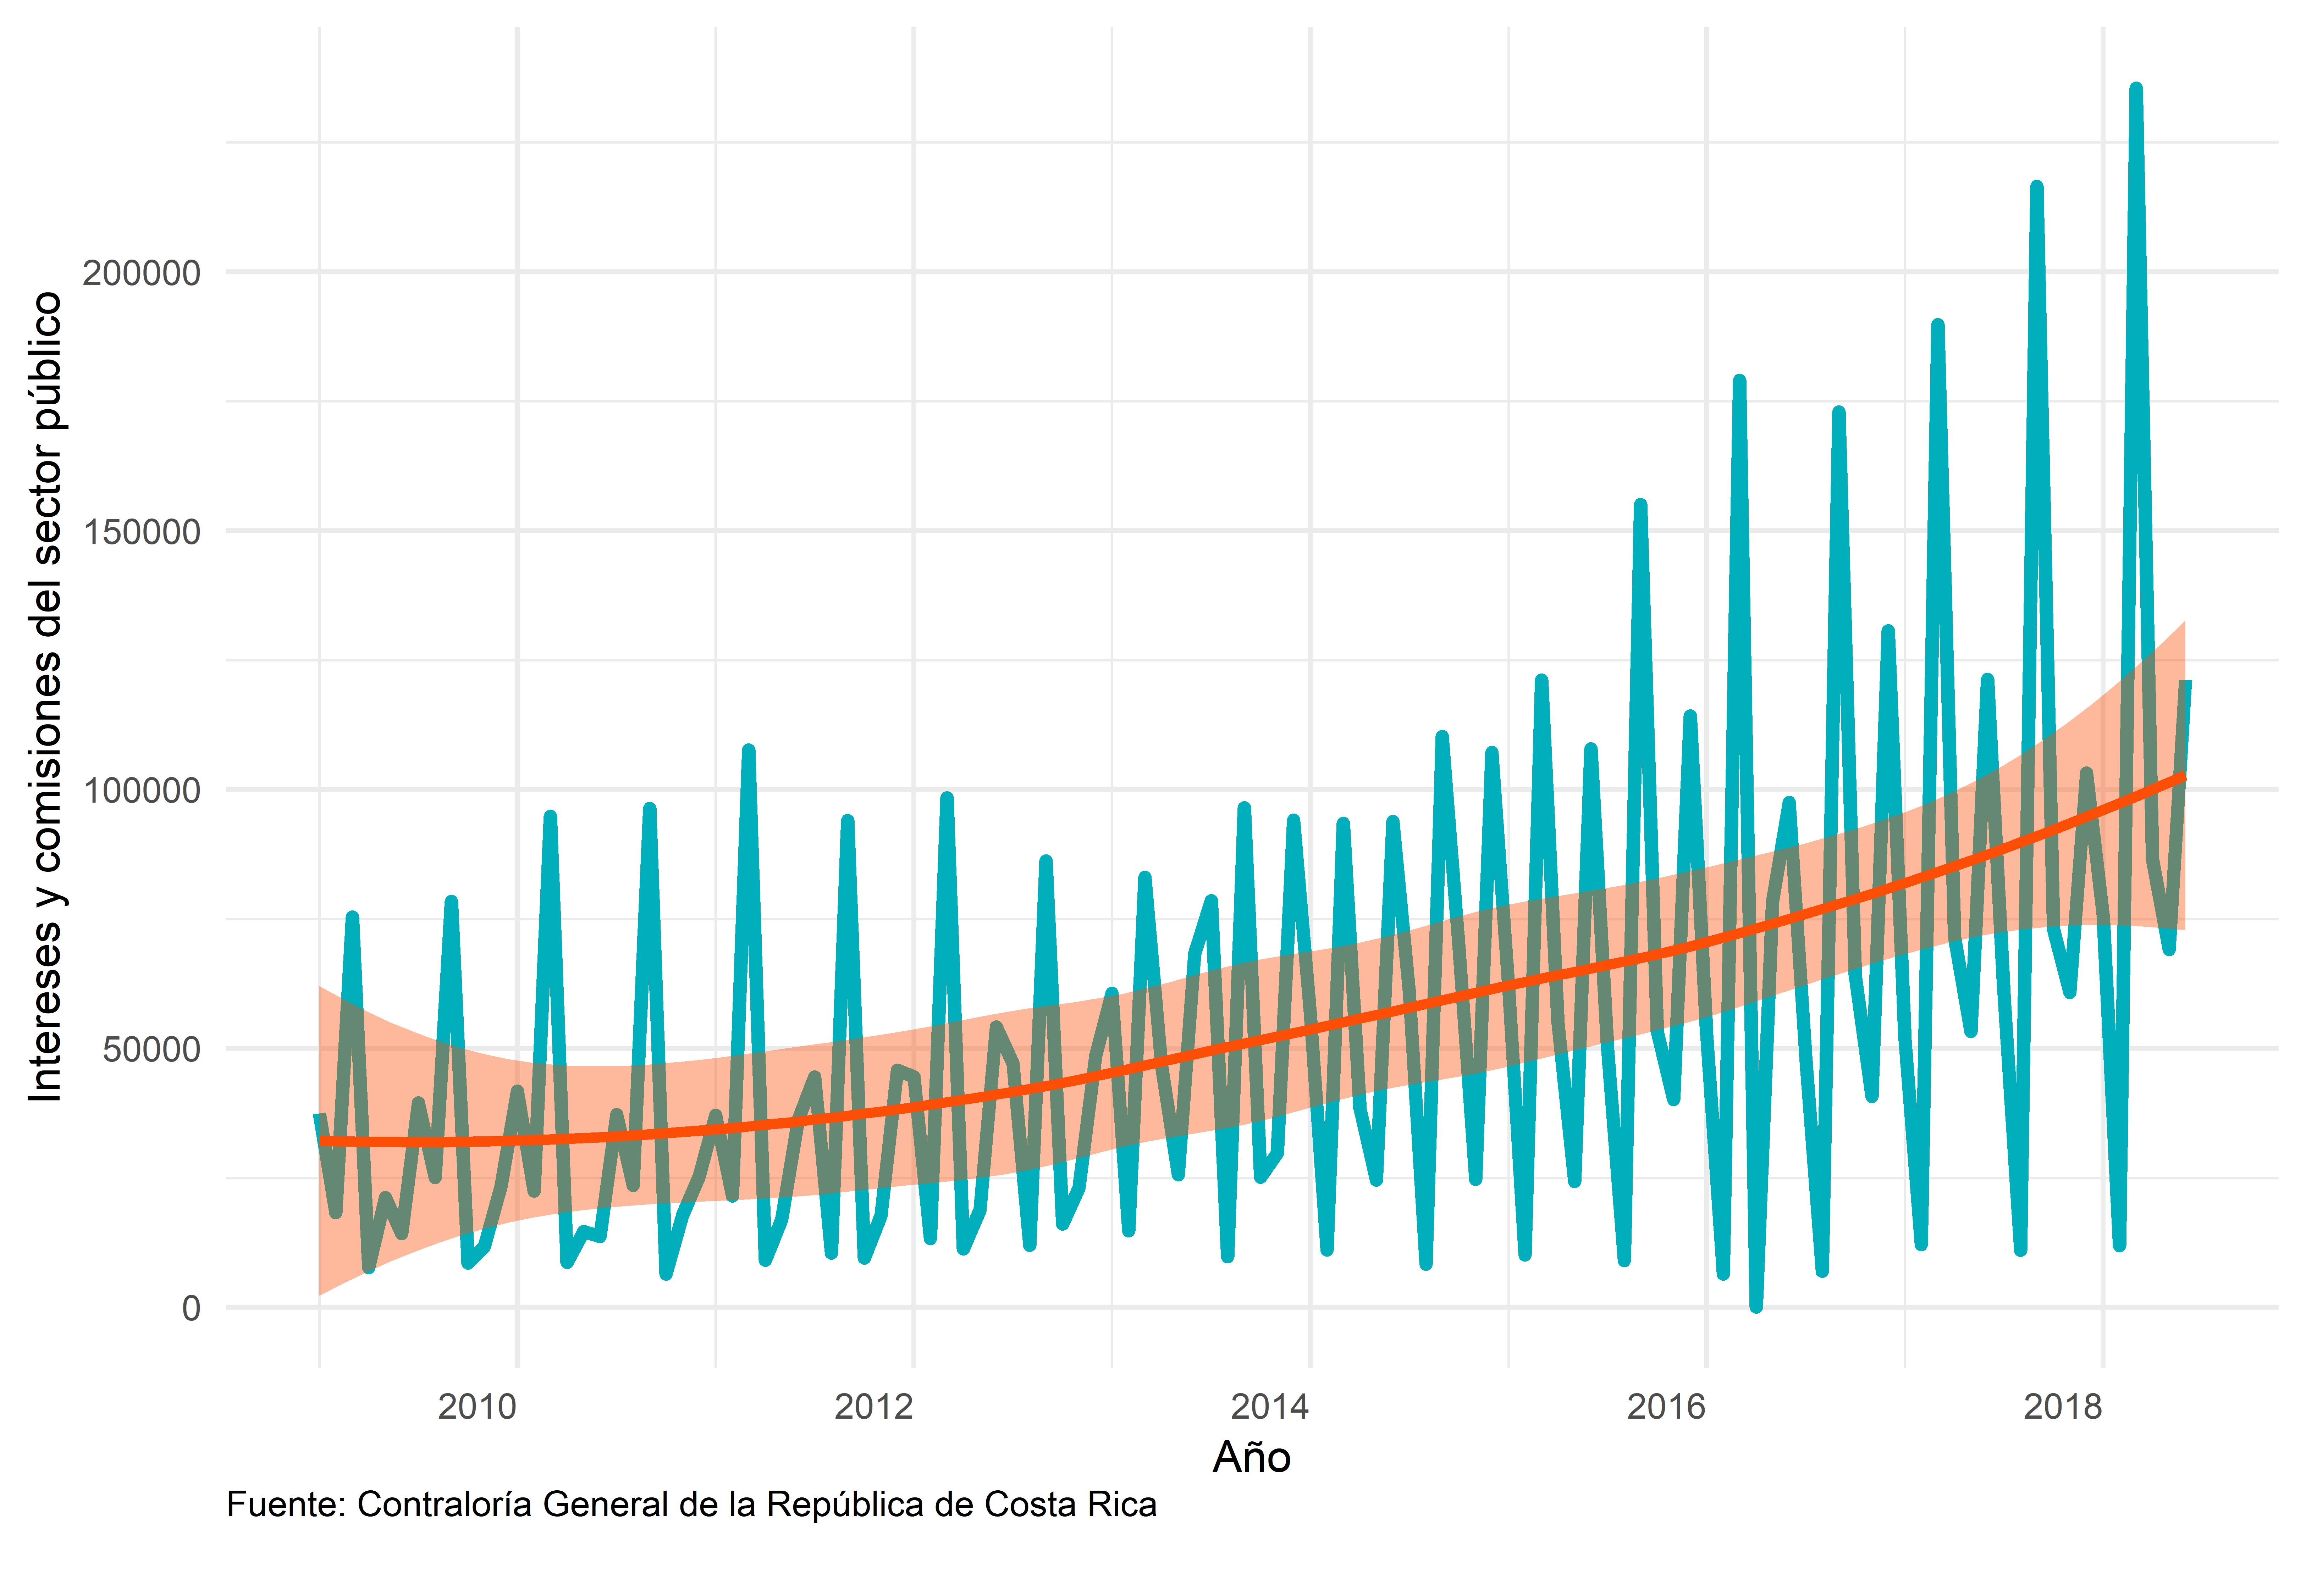
\includegraphics[width=1\linewidth,height=1\textheight]{Tesis_files/figure-latex/interesesplotgeneral-1} \caption{Intereses y comisiones del sector público en el periodo 2007-2018}\label{fig:interesesplotgeneral}
\end{figure}

\begin{figure}[!h]
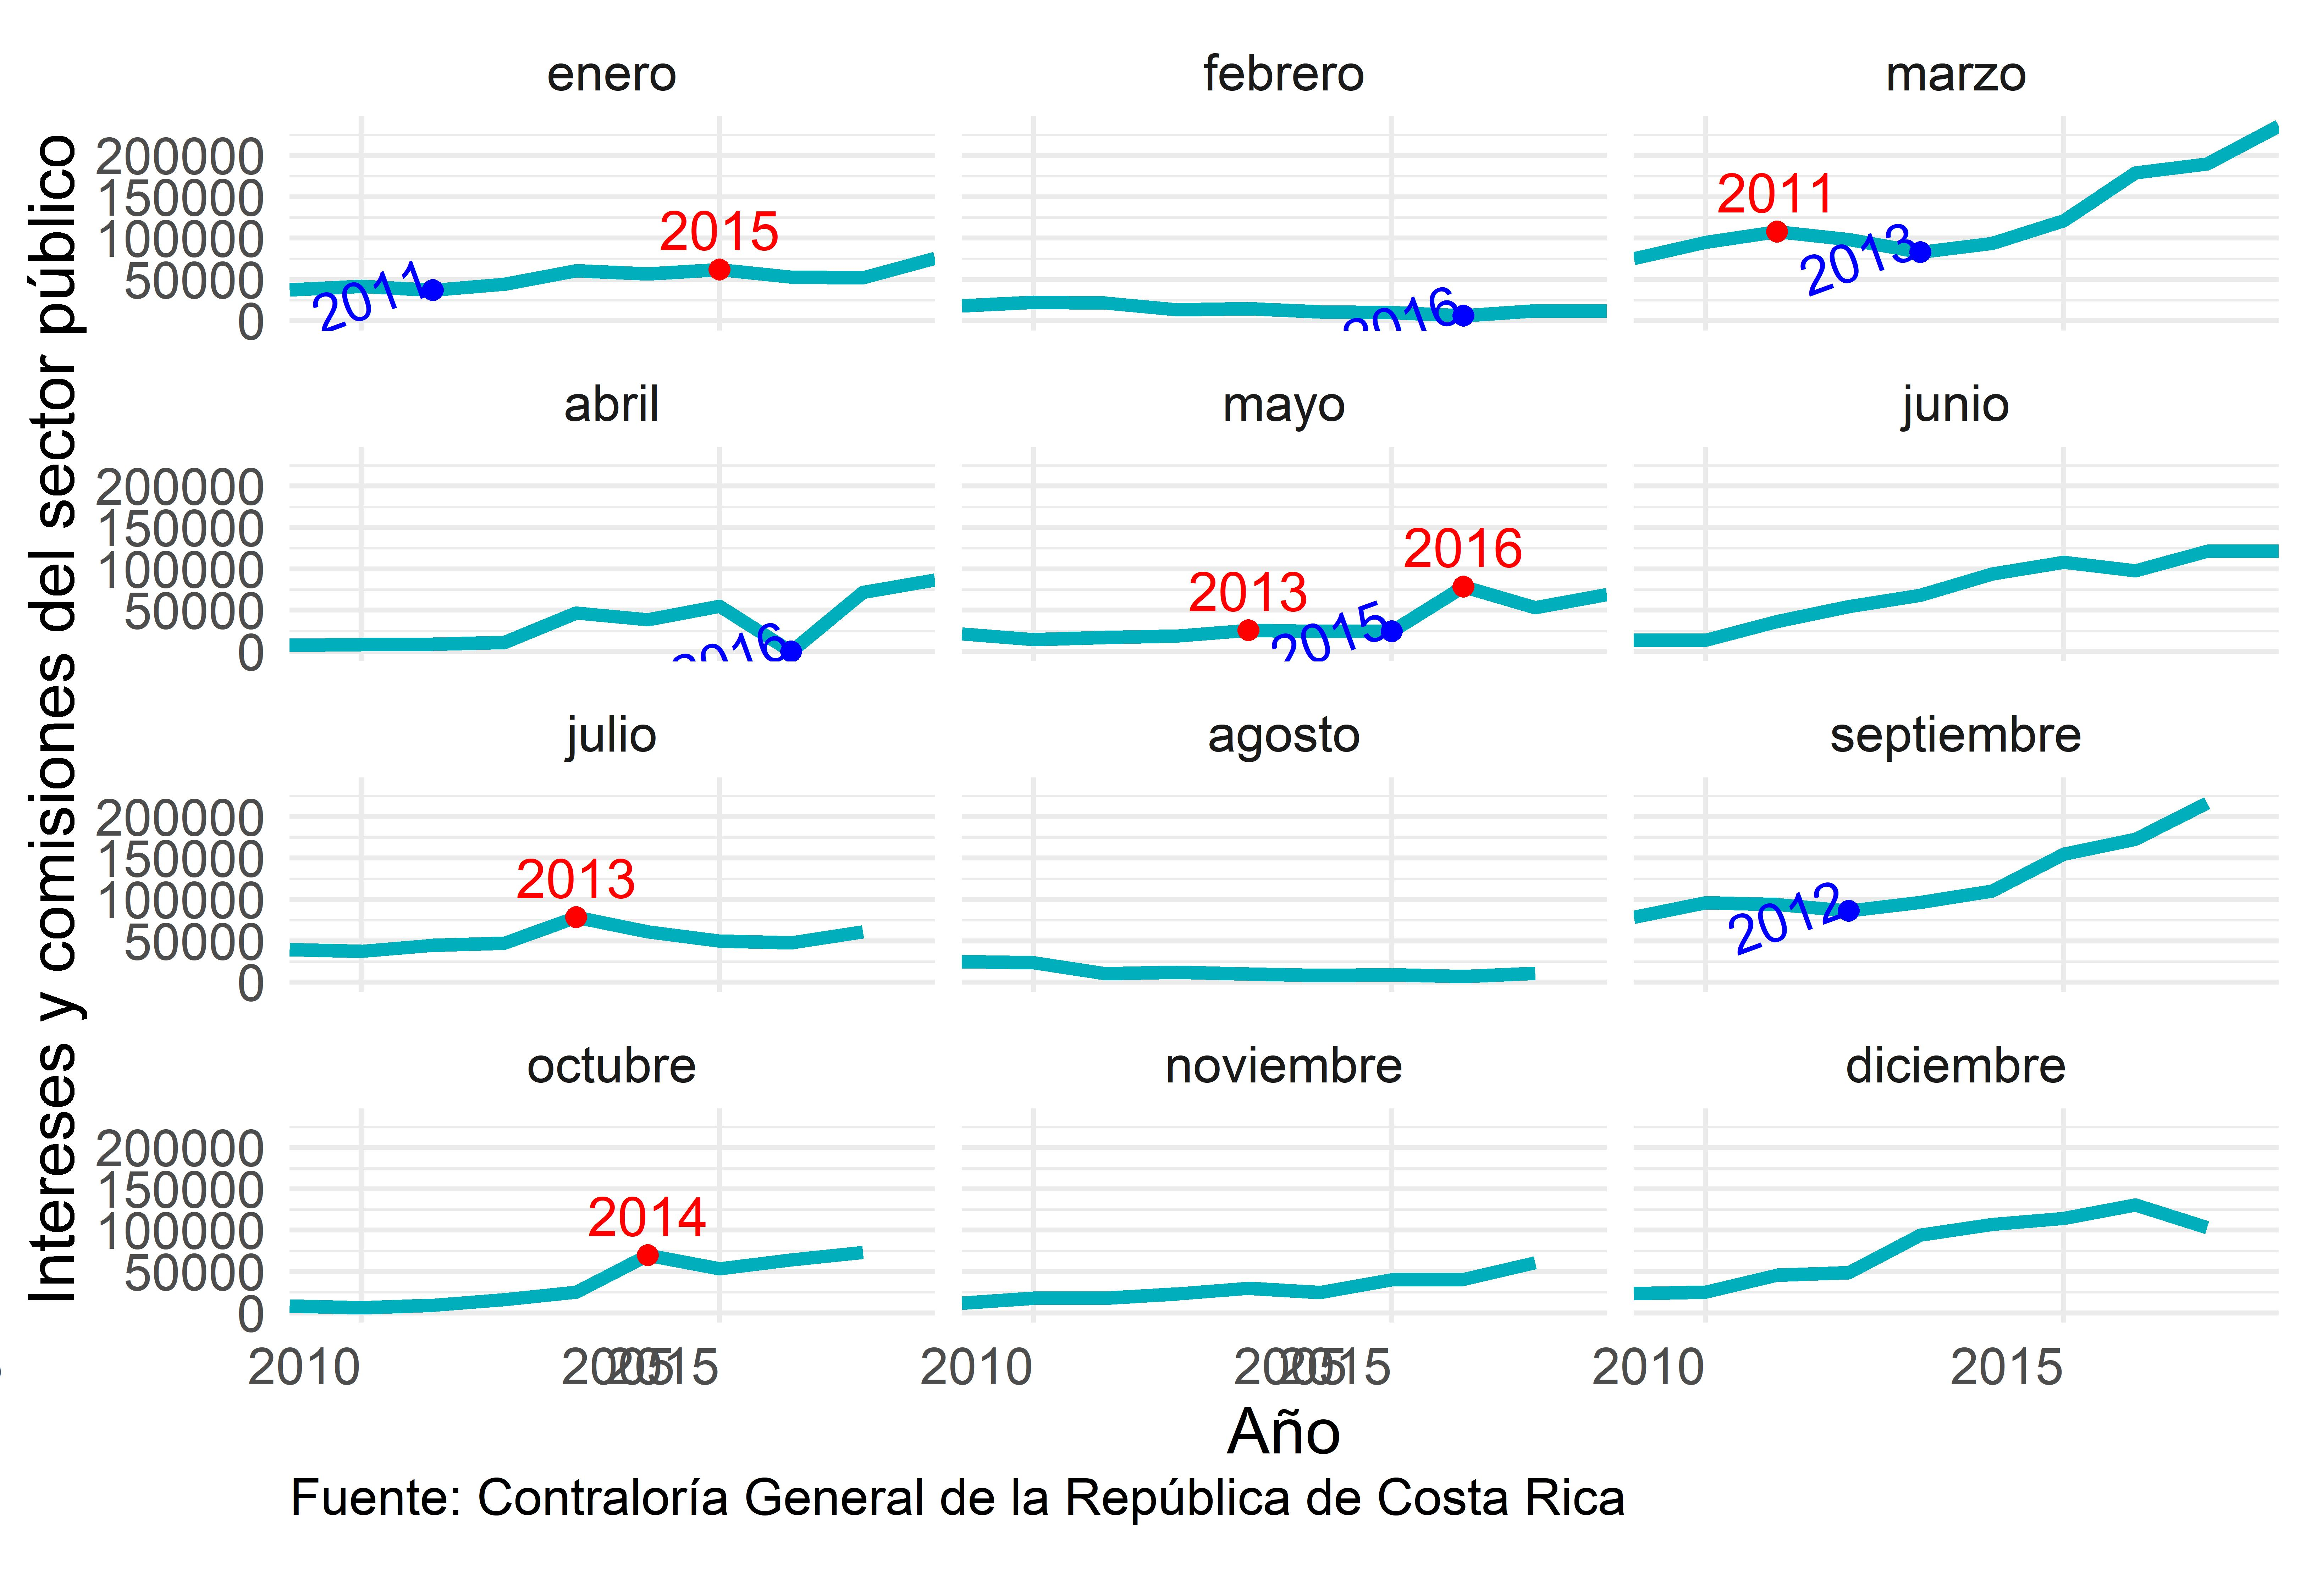
\includegraphics[width=1\linewidth,height=1\textheight]{Tesis_files/figure-latex/interesesplotperiodos-1} \caption{Intereses y comisiones del sector público en el periodo 2007-2018 según mes}\label{fig:interesesplotperiodos}
\end{figure}

En la figura \ref{fig:interesesplotdescomposicion} se muestra la
descomposición de la serie en sus distintos componentes. Pueden
observarse, además de un crecimiento a lo largo del tiempo posterior a
una disminución, los picos y las caídas en la parte estacional. El
componente aleatorio muestra indicios de que la variabilidad de la serie
no es homogénea, sino que cambia conforme pasa el tiempo, pues durante
un tiempo se mantuvo relativamente estable pero luego presenta algunos
cambios.

\begin{figure}[!h]
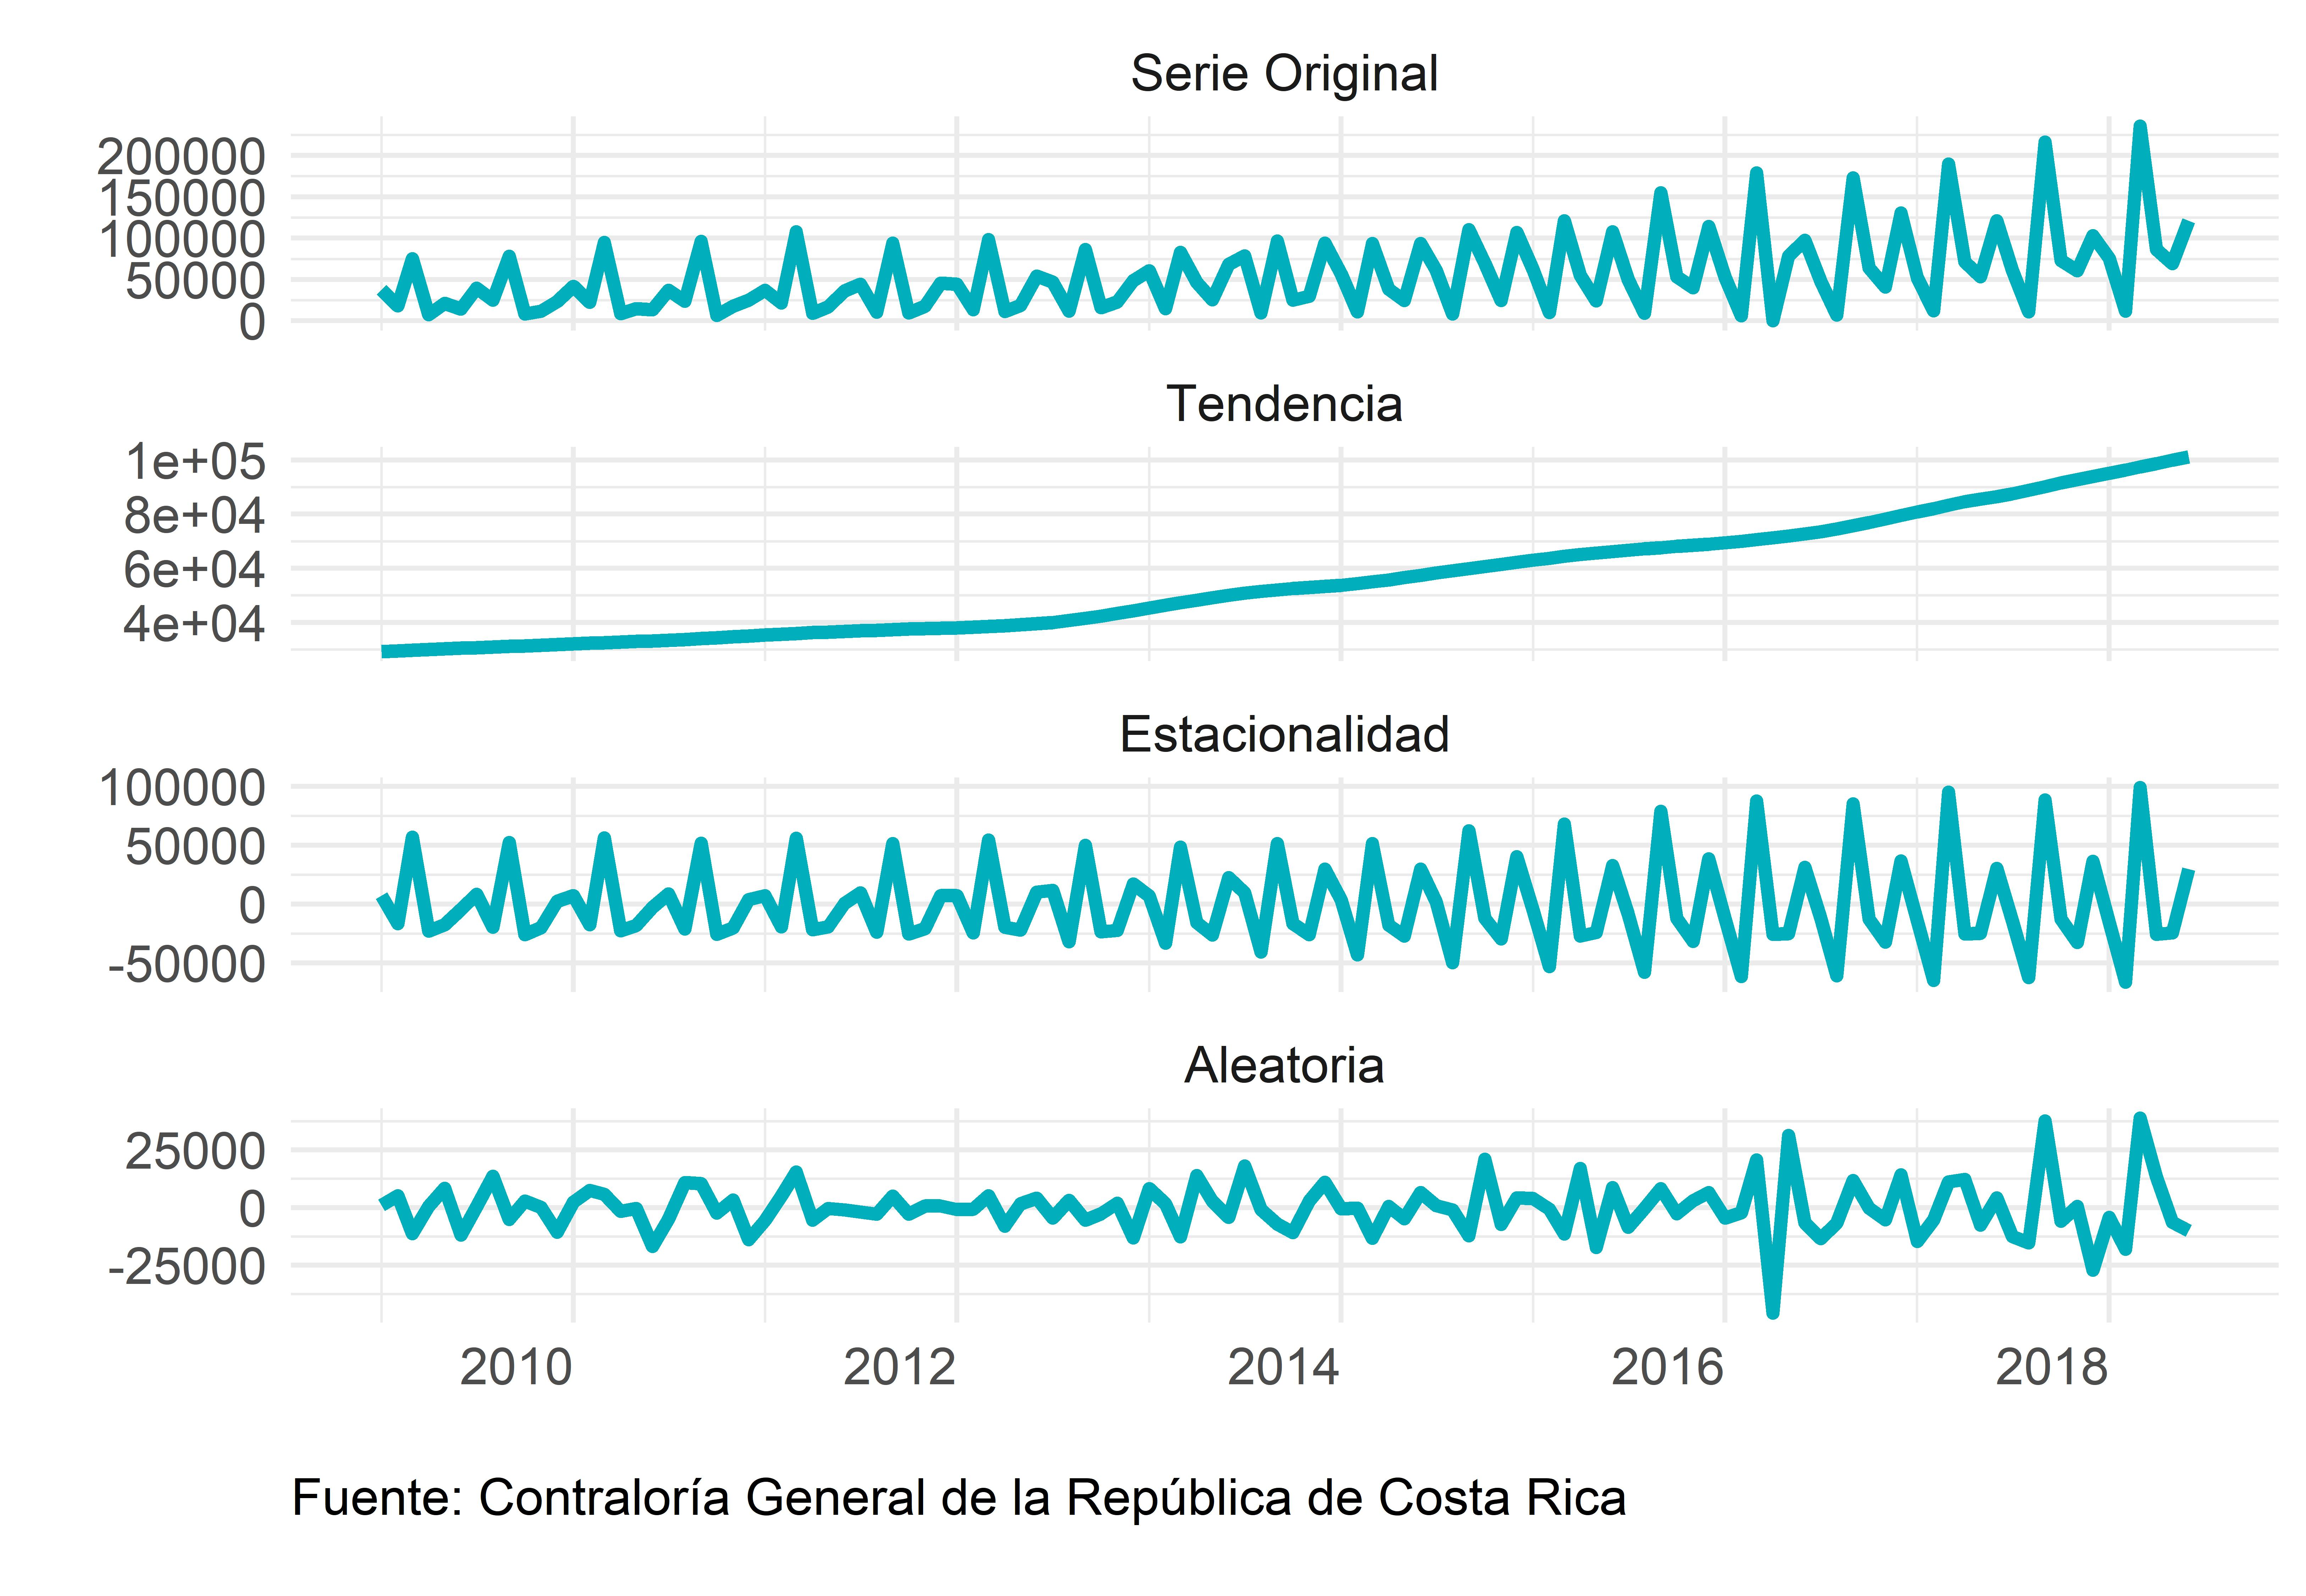
\includegraphics[width=1\linewidth,height=1\textheight]{Tesis_files/figure-latex/interesesplotdescomposicion-1} \caption{Descomposición de la serie de Incentivos salariales en el periodo 2007 - 2018}\label{fig:interesesplotdescomposicion}
\end{figure}

Por último, los modelos ajustados para pronosticar los intereses y
comisiones del sector público con un \(ARIMA(0,0,1)(0,1,0)_{12}\) para
el caso de la función \texttt{auto.arima()}; y un
\(ARIMA(0,1,2)(0,1,0)_{12}\) En este caso, la sobreparametrización es
superior en dos de las tres medidas de rendimiento tal y como muestra el
cuadro \ref{tab:interesesmedidas}, mientras que la figura
\ref{fig:interesesplotpronostico} muestra de manera gráfica los
pronósticos obtenidos, que son bastante similares pues ambos modelos
difieren solamente en un parámetro para la parte estacional.

\begin{table}[!h]

\caption{\label{tab:unnamed-chunk-19}\label{tab:interesesmedidas}Medidas de rendimiento según método de estimación para los intereses y comisiones del sector público}
\centering
\resizebox{\linewidth}{!}{
\begin{tabu} to \linewidth {>{\raggedleft}X>{\raggedleft}X>{\raggedleft}X>{\raggedleft}X}
\toprule
Método & RMSE & MAE & MAPE\\
\midrule
autoarima & 27737.53 & 19562.58 & 35.66424\\
sobreparametrizacion & 27280.46 & 19346.25 & 39.89648\\
\bottomrule
\end{tabu}}
\end{table}

\begin{figure}[!h]
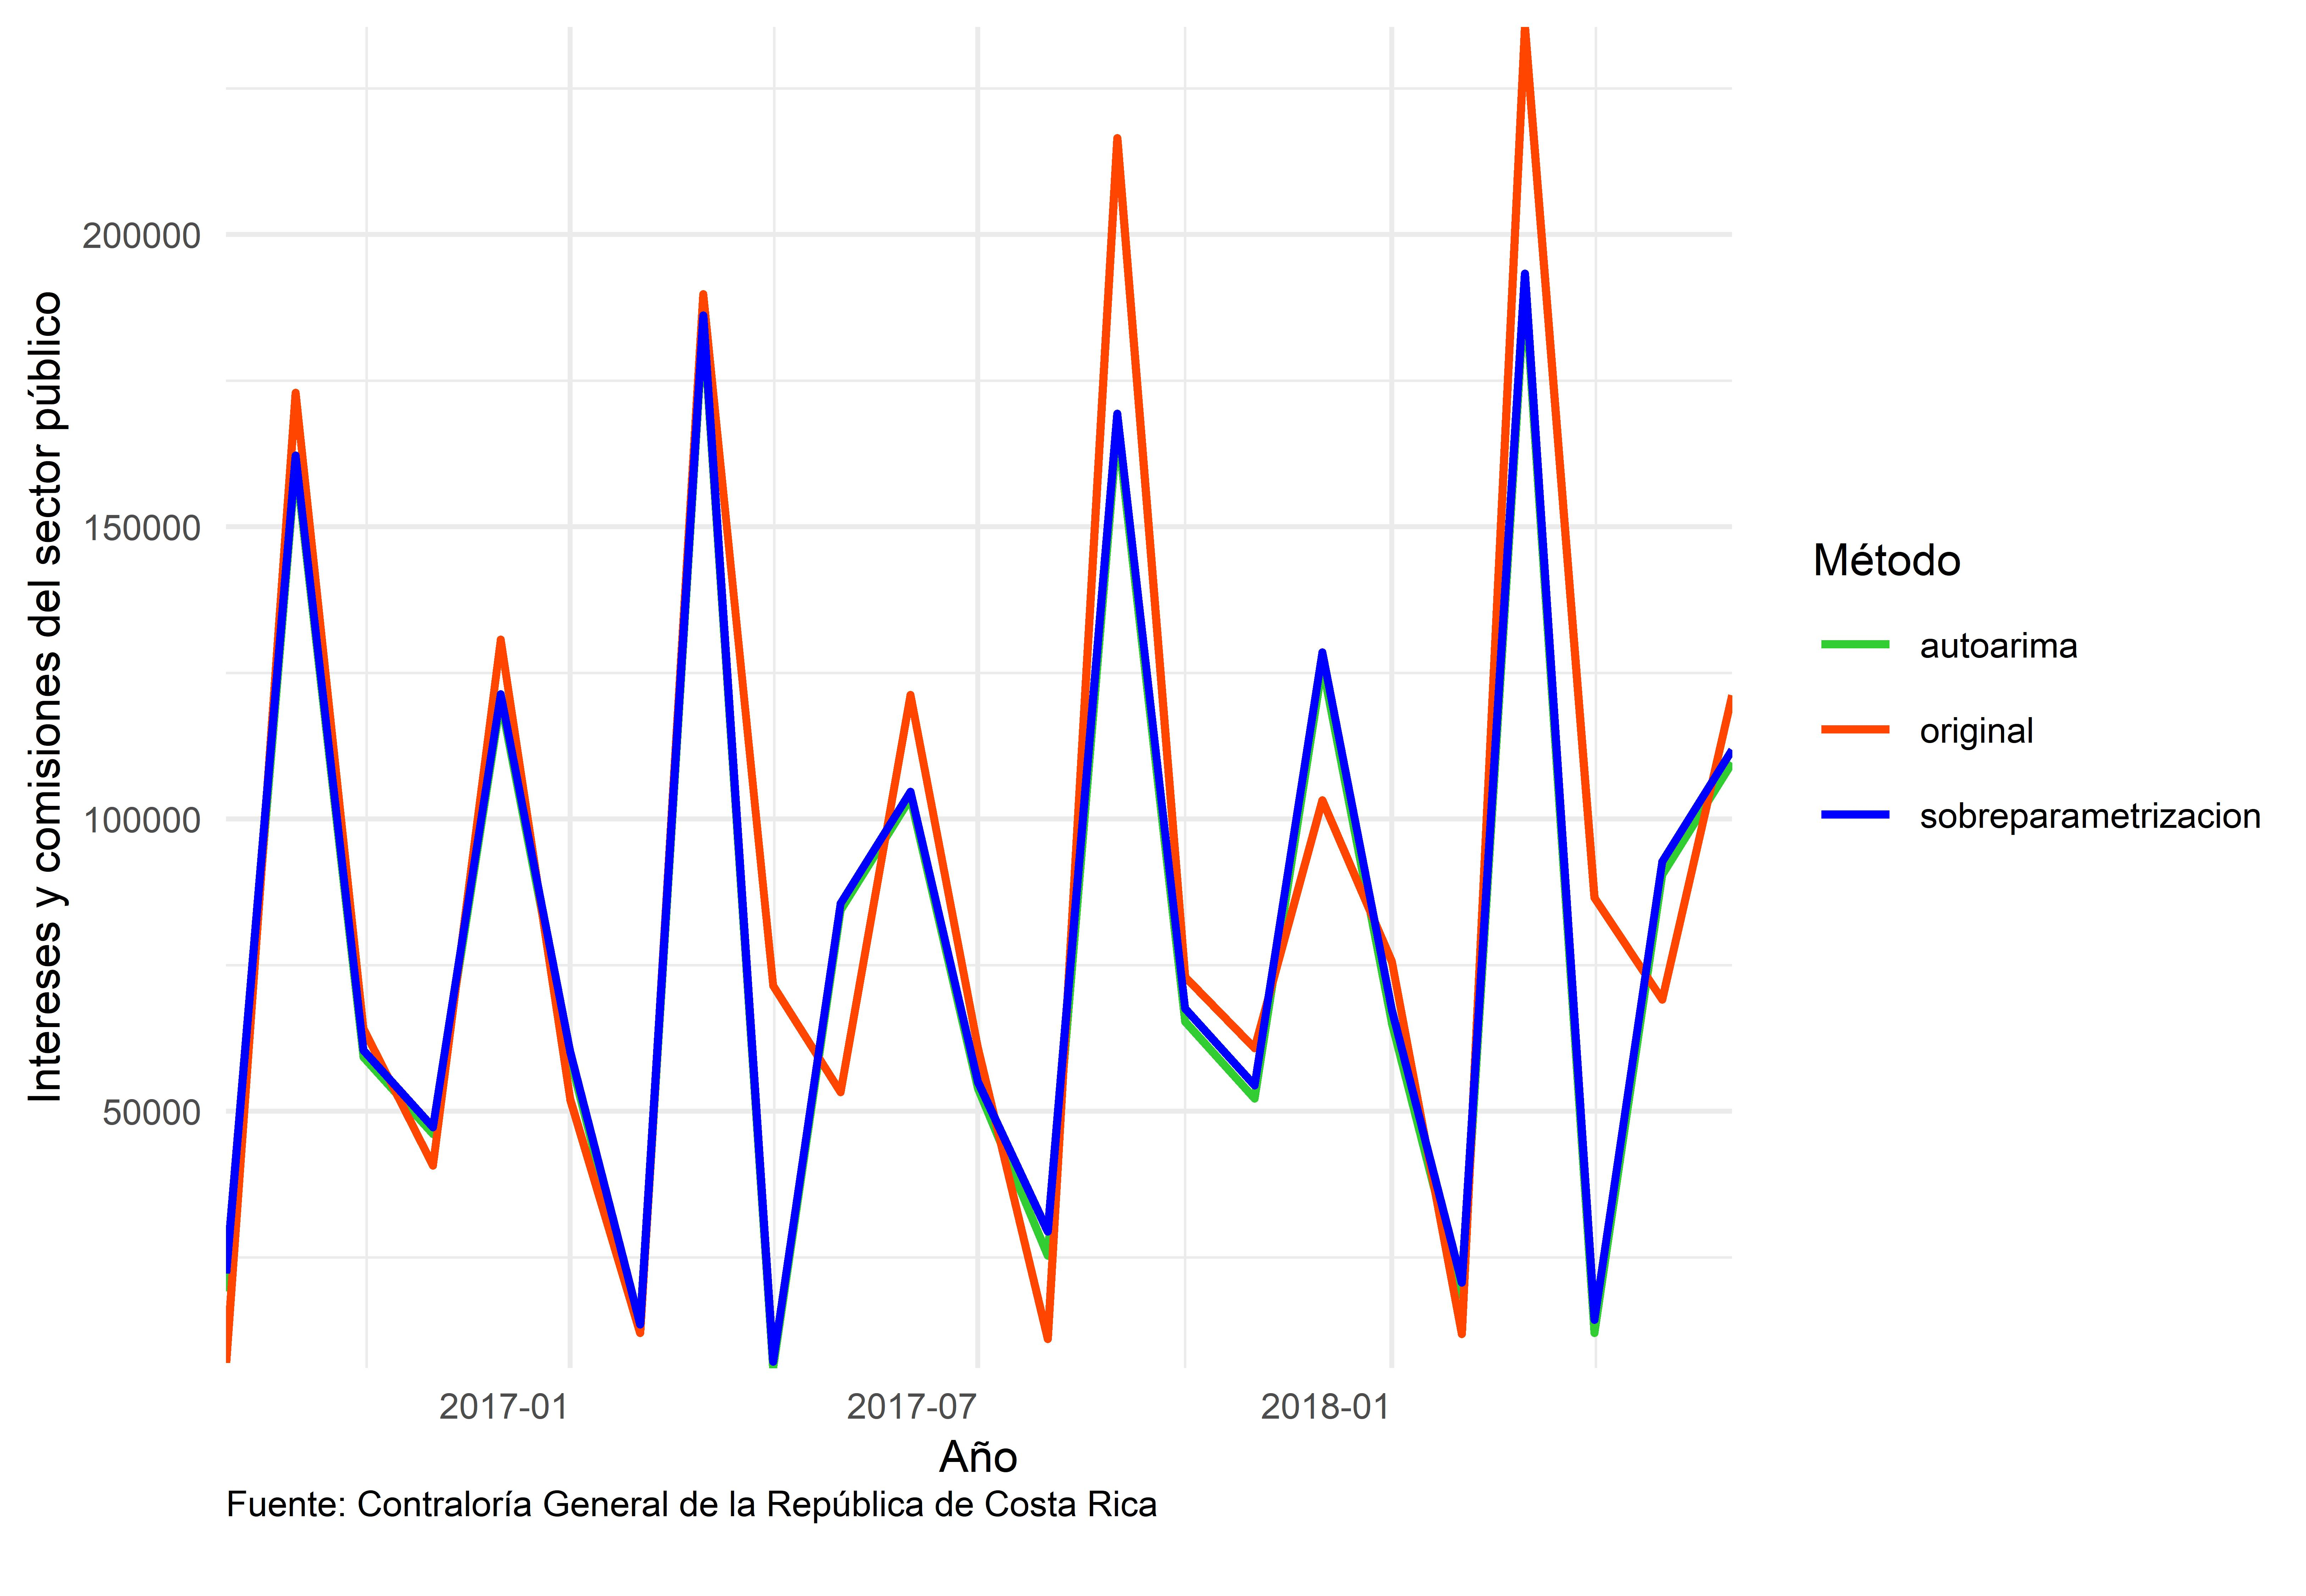
\includegraphics[width=1\linewidth,height=1\textheight]{Tesis_files/figure-latex/interesesplotpronostico-1} \caption{Pronósticos de los intereses y comisiones del sector público según método de estimación}\label{fig:interesesplotpronostico}
\end{figure}

\newpage

\section{CONCLUSIONES}

La presente investigación ha cubierto las bases fundamentales
relacionadas al análisis de series cronológicas. Se ha realizado una
recapitulación histórica de esta rama de la estadística y se han puesto
en evidencia uno de los principales problemas de las series de tiempo,
como lo es la subjetividad del observador en la selección de modelos. Es
ante este inconveniente que la investigación buscó siempre proponer un
aporte metodológico para la selección de modelos ARIMA y por ende, una
mejora en los pronósticos obtenidos a partir de estos modelos.

El uso de la sobreparametrización propuesto mediante un algoritmo de
selección de modelos ha sido implementado de la forma esperada, pues la
evaluación de los resultados al incorporar coeficientes al modelo se
puso a prueba tanto en series cronológicas simuladas como en datos
reales. El método propuesto implementado en las funciones del lenguaje R
permite evaluar una gama más amplia de modelos ARIMA al definir un
máximo en la cantidad de parámetros para las partes estacionales y no
estacionales de la series cronológicas, pues al definir este máximo se
definen todos los posibles escenarios que posteriormente evalúan el
aporte de cada nuevo término a los pronósticos. La incorporación de
estos nuevos parámetros en los modelos ARIMA son validados mediante
pruebas de significancia estadística, particiones de la serie
cronológica, medidas de bondad de ajuste de los modelos y sus
correspondientes medidas de rendimiento.

Como parte de la investigación, la series cronológicas utilizadas de
forma simulada y generadas a partir de registros administrativos
muestran como el uso de la sobreparametrización iguala y en muchos casos
mejora la calidad de los pronósticos obtenidos en comparación a métodos
ya establecidos, como es el caso de la función \texttt{auto.arima()}, o
estimación de modelos más genéricos con un bajo número de parámetros,
como los modelos estándar \(ARIMA(1,1,1)\) o
\(ARIMA(1,1,1)(1,1,1)_{12}\).

Como puede apreciarse en los resultados, al tener datos que vienen de un
proceso con bajo número de parámetros, el uso de la sobreparametrización
logra captar de buena manera el comportamiento de la serie y, además,
cuando el proceso que gobierna la serie es de un mayor grado, la
metodología propuesta, al considerar un mayor espectro paramétrico, es
capaz de capturar de buena forma el comportamiento de la serie y
conseguir pronósticos con una precisión mayor al de los métodos más
tradicionales. Lo anterior representa una mejora en cuanto a la
utilización de modelos ARIMA para el pronóstico de series cronológicas,
lo cual a su vez aporta herramientas para la toma de decisiones
relacionadas a este tipo de análisis.

Una potencial mejora al uso de la sobreparametrización es la inclusión
semi-automática de regresores para controlar cambios estructurales de la
serie cronológica en estudio, pues estos coeficientes adicionales
podrían controlar cambios particulares en la serie y que podrían mejorar
la precisión de los pronósticos.

La metodología aquí propuesta se encuentra disponible de manera abierta
mediante el paquete de R \texttt{popstudy}, el cual fue desarrollado
para esta investigación y cuenta con los procedimientos previamente
descritos. Se encuentra disponible en un repositorio de
Github\footnote{\url{https://github.com/cgamboasanabria/popstudy}} y
además en el repositorio CRAN\footnote{Publicación pendiente.}, que es
la fuente oficial de los paquetes del lenguaje R.

\newpage

\section{ANEXOS}

\subsection{Función de sobreparametrización}

\captionof{chunk}{Función op.arima}\label{funcion_op_arima}

\begin{Shaded}
\begin{Highlighting}[]
\NormalTok{op.arima }\OtherTok{\textless{}{-}} \ControlFlowTok{function}\NormalTok{(}\AttributeTok{arima\_process =} \FunctionTok{c}\NormalTok{(}\AttributeTok{p =} \DecValTok{1}\NormalTok{, }\AttributeTok{d =} \DecValTok{1}\NormalTok{, }\AttributeTok{q =} \DecValTok{1}\NormalTok{,}
                                       \AttributeTok{P =} \DecValTok{1}\NormalTok{, }\AttributeTok{D =} \DecValTok{1}\NormalTok{, }\AttributeTok{Q =} \DecValTok{1}\NormalTok{),}
\NormalTok{                     seasonal\_periodicity,}
\NormalTok{                     time\_serie, }\AttributeTok{reg =} \ConstantTok{NULL}\NormalTok{, }\AttributeTok{horiz =} \DecValTok{12}\NormalTok{,}
                     \AttributeTok{prop=}\NormalTok{.}\DecValTok{8}\NormalTok{, }\AttributeTok{training\_weight=}\NormalTok{.}\DecValTok{2}\NormalTok{, }\AttributeTok{testing\_weight=}\NormalTok{.}\DecValTok{8}\NormalTok{,}
                     \AttributeTok{parallelize=}\ConstantTok{FALSE}\NormalTok{,}
                     \AttributeTok{clusters=}\FunctionTok{detectCores}\NormalTok{(}\AttributeTok{logical =} \ConstantTok{FALSE}\NormalTok{),...)\{}

\NormalTok{    data\_partition }\OtherTok{\textless{}{-}} \FunctionTok{round}\NormalTok{(}\FunctionTok{length}\NormalTok{(time\_serie)}\SpecialCharTok{*}\NormalTok{prop, }\DecValTok{0}\NormalTok{)}
\NormalTok{    train }\OtherTok{\textless{}\textless{}{-}} \FunctionTok{subset}\NormalTok{(time\_serie, }\AttributeTok{end=}\NormalTok{data\_partition)}
\NormalTok{    test }\OtherTok{\textless{}\textless{}{-}} \FunctionTok{subset}\NormalTok{(time\_serie, }\AttributeTok{start=}\NormalTok{data\_partition}\SpecialCharTok{+}\DecValTok{1}\NormalTok{)}

\NormalTok{    arima\_model }\OtherTok{\textless{}{-}} \ControlFlowTok{function}\NormalTok{(time\_serie, non\_seasonal, seasonal, periodic, }
                            \AttributeTok{regr =} \ConstantTok{NULL}\NormalTok{,...)\{}

        \ControlFlowTok{if}\NormalTok{(}\FunctionTok{is.list}\NormalTok{(non\_seasonal))\{}
\NormalTok{            non\_seasonal }\OtherTok{\textless{}{-}} \FunctionTok{unlist}\NormalTok{(non\_seasonal)}
\NormalTok{        \}}

        \ControlFlowTok{if}\NormalTok{(}\FunctionTok{is.list}\NormalTok{(seasonal))\{}
\NormalTok{            seasonal }\OtherTok{\textless{}{-}} \FunctionTok{unlist}\NormalTok{(seasonal)}
\NormalTok{        \}}

\NormalTok{        seasonal\_part }\OtherTok{\textless{}{-}} \FunctionTok{list}\NormalTok{(}\AttributeTok{order=}\NormalTok{seasonal, }\AttributeTok{period=}\NormalTok{periodic)}
        \ControlFlowTok{if}\NormalTok{(}\FunctionTok{is.null}\NormalTok{(regr))\{}
\NormalTok{            arima\_model }\OtherTok{\textless{}{-}} \FunctionTok{tryCatch}\NormalTok{(\{}
                \FunctionTok{Arima}\NormalTok{(time\_serie,}
                      \AttributeTok{order =}\NormalTok{ non\_seasonal,}
                      \AttributeTok{seasonal =}\NormalTok{ seasonal\_part,...)}
\NormalTok{            \},}
            \AttributeTok{error =} \ControlFlowTok{function}\NormalTok{(e) }\ConstantTok{NULL}\NormalTok{)}
\NormalTok{        \}}

        \ControlFlowTok{if}\NormalTok{(}\SpecialCharTok{!}\FunctionTok{is.null}\NormalTok{(regr))\{}
\NormalTok{            arima\_model }\OtherTok{\textless{}{-}}\FunctionTok{tryCatch}\NormalTok{(\{}
                \FunctionTok{Arima}\NormalTok{(time\_serie,}
                      \AttributeTok{order =}\NormalTok{ non\_seasonal,}
                      \AttributeTok{seasonal =}\NormalTok{ seasonal\_part,}
                      \AttributeTok{xreg =}\NormalTok{ regr,...)}
\NormalTok{            \},}
            \AttributeTok{error =} \ControlFlowTok{function}\NormalTok{(e) }\ConstantTok{NULL}\NormalTok{)}
\NormalTok{        \}}

        \ControlFlowTok{if}\NormalTok{(}\SpecialCharTok{!}\FunctionTok{is.null}\NormalTok{(arima\_model))\{}
\NormalTok{            degrees\_of\_freedom }\OtherTok{\textless{}{-}}\NormalTok{ arima\_model}\SpecialCharTok{$}\NormalTok{nobs }\SpecialCharTok{{-}} \FunctionTok{length}\NormalTok{(arima\_model}\SpecialCharTok{$}\NormalTok{coef)}
\NormalTok{            t\_value }\OtherTok{\textless{}{-}}\NormalTok{ arima\_model}\SpecialCharTok{$}\NormalTok{coef}\SpecialCharTok{/}\FunctionTok{sqrt}\NormalTok{(}\FunctionTok{diag}\NormalTok{(arima\_model}\SpecialCharTok{$}\NormalTok{var.coef))}
\NormalTok{            prob }\OtherTok{\textless{}{-}}\NormalTok{ stats}\SpecialCharTok{::}\FunctionTok{pf}\NormalTok{(t\_value}\SpecialCharTok{\^{}}\DecValTok{2}\NormalTok{, }\AttributeTok{df1 =} \DecValTok{1}\NormalTok{, }\AttributeTok{df2 =}\NormalTok{ degrees\_of\_freedom, }
                              \AttributeTok{lower.tail =} \ConstantTok{FALSE}\NormalTok{)}
            \FunctionTok{ifelse}\NormalTok{(}\FunctionTok{sum}\NormalTok{(}\DecValTok{1}\SpecialCharTok{*}\NormalTok{prob}\SpecialCharTok{\textgreater{}}\FloatTok{0.05}\NormalTok{)}\SpecialCharTok{\textless{}}\DecValTok{1}\NormalTok{, }\FunctionTok{return}\NormalTok{(arima\_model), }\DecValTok{1}\NormalTok{)}
\NormalTok{        \}}

\NormalTok{    \}}

\NormalTok{    arima\_measures }\OtherTok{\textless{}{-}} \ControlFlowTok{function}\NormalTok{(arima\_model, testing, horizon, }\AttributeTok{regr =} \ConstantTok{NULL}\NormalTok{)\{}

\NormalTok{        model\_spec }\OtherTok{\textless{}{-}} \FunctionTok{capture.output}\NormalTok{(arima\_model)}
\NormalTok{        model\_spec }\OtherTok{\textless{}{-}} \FunctionTok{substr}\NormalTok{(model\_spec[}\DecValTok{2}\NormalTok{],}\DecValTok{1}\NormalTok{, }\DecValTok{23}\NormalTok{)}

     
\NormalTok{        data }\OtherTok{\textless{}{-}} \FunctionTok{capture.output}\NormalTok{(}\FunctionTok{summary}\NormalTok{(arima\_model))}
\NormalTok{        data }\OtherTok{\textless{}{-}}\NormalTok{ data[}\FunctionTok{grepl}\NormalTok{(}\StringTok{"AIC"}\NormalTok{, data) }\SpecialCharTok{==}\NormalTok{ T]}
\NormalTok{        model\_info }\OtherTok{\textless{}{-}} \FunctionTok{strsplit}\NormalTok{(data, }\StringTok{" "}\NormalTok{)}
\NormalTok{        pos }\OtherTok{\textless{}{-}} \FunctionTok{which}\NormalTok{(}\FunctionTok{sapply}\NormalTok{(model\_info, nchar)}\SpecialCharTok{\textgreater{}}\DecValTok{0}\NormalTok{)}
\NormalTok{        model\_info }\OtherTok{\textless{}{-}}\NormalTok{ model\_info[[}\DecValTok{1}\NormalTok{]][pos]}
\NormalTok{        model\_info }\OtherTok{\textless{}{-}} \FunctionTok{do.call}\NormalTok{(}\StringTok{"rbind"}\NormalTok{, }\FunctionTok{strsplit}\NormalTok{(model\_info, }\StringTok{"="}\NormalTok{)) }\SpecialCharTok{\%\textgreater{}\%}
            \FunctionTok{data.frame}\NormalTok{()}
        \FunctionTok{colnames}\NormalTok{(model\_info) }\OtherTok{\textless{}{-}} \FunctionTok{c}\NormalTok{(}\StringTok{"Medida"}\NormalTok{, }\StringTok{"Valor"}\NormalTok{)}
\NormalTok{        model\_info }\OtherTok{\textless{}{-}}\NormalTok{ model\_info }\SpecialCharTok{\%\textgreater{}\%}
            \FunctionTok{mutate}\NormalTok{(}\AttributeTok{Valor =} \FunctionTok{as.numeric}\NormalTok{(}\FunctionTok{as.character}\NormalTok{(Valor))) }\SpecialCharTok{\%\textgreater{}\%}
            \FunctionTok{spread}\NormalTok{(Medida, Valor) }\SpecialCharTok{\%\textgreater{}\%}
            \FunctionTok{data.frame}\NormalTok{(}\AttributeTok{arima\_model =}\NormalTok{ model\_spec)}

\NormalTok{        model\_performance }\OtherTok{\textless{}{-}} \FunctionTok{data.frame}\NormalTok{(}\AttributeTok{arima\_model =} \FunctionTok{c}\NormalTok{(model\_spec, }
                                                        \FunctionTok{paste}\NormalTok{(model\_spec,}
                                                              \StringTok{"Validacion"}\NormalTok{)),}
                                        \FunctionTok{accuracy}\NormalTok{(}\FunctionTok{forecast}\NormalTok{(arima\_model, horizon, }
                                                          \AttributeTok{xreg =}\NormalTok{ regr),}
\NormalTok{                                                 testing))}
        \FunctionTok{merge}\NormalTok{(model\_info, model\_performance, }\AttributeTok{by=}\StringTok{"arima\_model"}\NormalTok{, }\AttributeTok{all =} \ConstantTok{TRUE}\NormalTok{) }\SpecialCharTok{\%\textgreater{}\%}
            \FunctionTok{select}\NormalTok{(arima\_model, AIC, AICc, BIC, MAE, RMSE, MASE)}
\NormalTok{    \}}

\NormalTok{    arima\_selected }\OtherTok{\textless{}{-}} \ControlFlowTok{function}\NormalTok{(model\_table, }\AttributeTok{Wtrain=}\NormalTok{training\_weight, }
                               \AttributeTok{Wtest=}\NormalTok{testing\_weight)\{}

\NormalTok{        model\_table }\OtherTok{\textless{}{-}}\NormalTok{ model\_table }\SpecialCharTok{\%\textgreater{}\%}
            \FunctionTok{distinct}\NormalTok{(arima\_model, }\AttributeTok{.keep\_all =} \ConstantTok{TRUE}\NormalTok{)}

\NormalTok{        model\_table }\OtherTok{\textless{}{-}}\NormalTok{ model\_table }\SpecialCharTok{\%\textgreater{}\%}
            \FunctionTok{mutate}\NormalTok{(}\AttributeTok{mod =} \FunctionTok{as.character}\NormalTok{(}\FunctionTok{c}\NormalTok{(}\DecValTok{0}\NormalTok{, }\FunctionTok{rep}\NormalTok{(}\DecValTok{1}\SpecialCharTok{:}\NormalTok{(}\FunctionTok{nrow}\NormalTok{(model\_table)}\SpecialCharTok{{-}}\DecValTok{1}\NormalTok{)}\SpecialCharTok{\%/\%}\DecValTok{2}\NormalTok{))))}

\NormalTok{        tabla2 }\OtherTok{\textless{}{-}}\NormalTok{ model\_table }\SpecialCharTok{\%\textgreater{}\%}
            \FunctionTok{mutate\_at}\NormalTok{(}\FunctionTok{vars}\NormalTok{(}\FunctionTok{contains}\NormalTok{(}\StringTok{"C"}\NormalTok{)), }\ControlFlowTok{function}\NormalTok{(x)\{x}\SpecialCharTok{{-}}\FunctionTok{min}\NormalTok{(x, }\AttributeTok{na.rm=}\ConstantTok{TRUE}\NormalTok{)\}) }\SpecialCharTok{\%\textgreater{}\%}
            \FunctionTok{mutate\_if}\NormalTok{(is.numeric, }\ControlFlowTok{function}\NormalTok{(x) }\FunctionTok{ifelse}\NormalTok{(}\FunctionTok{is.na}\NormalTok{(x),}\DecValTok{0}\NormalTok{,x)) }\SpecialCharTok{\%\textgreater{}\%}
            \FunctionTok{mutate}\NormalTok{(}\AttributeTok{puntaje =}\NormalTok{ AIC}\SpecialCharTok{+}\NormalTok{AICc}\SpecialCharTok{+}\NormalTok{BIC}\SpecialCharTok{+}\NormalTok{MAE}\SpecialCharTok{+}\NormalTok{RMSE}\SpecialCharTok{+}\NormalTok{MASE,}
                   \AttributeTok{ponde =} \FunctionTok{ifelse}\NormalTok{(}\FunctionTok{grepl}\NormalTok{(}\StringTok{"Validacion"}\NormalTok{, arima\_model)}\SpecialCharTok{==}\ConstantTok{TRUE}\NormalTok{,}
\NormalTok{                                  Wtest, Wtrain),}
                   \AttributeTok{puntaje =}\NormalTok{ puntaje}\SpecialCharTok{*}\NormalTok{ponde)}

        \FunctionTok{suppressMessages}\NormalTok{(\{}
\NormalTok{            minimal\_score }\OtherTok{\textless{}{-}}\NormalTok{ tabla2 }\SpecialCharTok{\%\textgreater{}\%}
                \FunctionTok{group\_by}\NormalTok{(mod) }\SpecialCharTok{\%\textgreater{}\%}
                \FunctionTok{summarise}\NormalTok{(}\AttributeTok{puntaje=}\FunctionTok{sum}\NormalTok{(puntaje)) }\SpecialCharTok{\%\textgreater{}\%}
\NormalTok{                ungroup}
\NormalTok{        \})}

\NormalTok{        pos }\OtherTok{\textless{}{-}}\NormalTok{ minimal\_score}\SpecialCharTok{$}\NormalTok{mod[}\FunctionTok{which}\NormalTok{(}
\NormalTok{          minimal\_score}\SpecialCharTok{$}\NormalTok{puntaje}\SpecialCharTok{==}\FunctionTok{min}\NormalTok{(minimal\_score}\SpecialCharTok{$}\NormalTok{puntaje))]}

\NormalTok{        model\_table }\SpecialCharTok{\%\textgreater{}\%}
            \FunctionTok{filter}\NormalTok{(mod }\SpecialCharTok{\%in\%}\NormalTok{ pos) }\SpecialCharTok{\%\textgreater{}\%}
\NormalTok{            dplyr}\SpecialCharTok{::}\FunctionTok{select}\NormalTok{(arima\_model}\SpecialCharTok{:}\NormalTok{MASE)}
\NormalTok{    \}}

    \FunctionTok{suppressWarnings}\NormalTok{(\{}
\NormalTok{        valores }\OtherTok{\textless{}{-}} \FunctionTok{expand.grid}\NormalTok{(}\AttributeTok{p =} \DecValTok{0}\SpecialCharTok{:}\NormalTok{arima\_process[}\DecValTok{1}\NormalTok{], }
                               \AttributeTok{d =} \DecValTok{0}\SpecialCharTok{:}\NormalTok{arima\_process[}\DecValTok{2}\NormalTok{], }
                               \AttributeTok{q =} \DecValTok{0}\SpecialCharTok{:}\NormalTok{arima\_process[}\DecValTok{3}\NormalTok{],}
                               \AttributeTok{P =} \DecValTok{0}\SpecialCharTok{:}\NormalTok{arima\_process[}\DecValTok{4}\NormalTok{], }
                               \AttributeTok{D =} \DecValTok{0}\SpecialCharTok{:}\NormalTok{arima\_process[}\DecValTok{5}\NormalTok{], }
                               \AttributeTok{Q =} \DecValTok{0}\SpecialCharTok{:}\NormalTok{arima\_process[}\DecValTok{6}\NormalTok{])}

\NormalTok{        non\_seasonal\_values }\OtherTok{\textless{}{-}} \FunctionTok{split}\NormalTok{(}\FunctionTok{as.matrix}\NormalTok{(valores[, }\DecValTok{1}\SpecialCharTok{:}\DecValTok{3}\NormalTok{]),}
                                     \FunctionTok{row}\NormalTok{(valores[, }\DecValTok{1}\SpecialCharTok{:}\DecValTok{3}\NormalTok{]))}
\NormalTok{        seasonal\_values }\OtherTok{\textless{}{-}} \FunctionTok{split}\NormalTok{(}\FunctionTok{as.matrix}\NormalTok{(valores[, }\DecValTok{4}\SpecialCharTok{:}\DecValTok{6}\NormalTok{]),}
                                 \FunctionTok{row}\NormalTok{(valores[, }\DecValTok{4}\SpecialCharTok{:}\DecValTok{6}\NormalTok{]))}

        \ControlFlowTok{if}\NormalTok{(parallelize}\SpecialCharTok{==}\ConstantTok{FALSE}\NormalTok{)\{}
\NormalTok{            arima\_models }\OtherTok{\textless{}{-}} \FunctionTok{mapply}\NormalTok{(arima\_model,}
                                   \AttributeTok{non\_seasonal=}\NormalTok{non\_seasonal\_values,}
                                   \AttributeTok{seasonal=}\NormalTok{seasonal\_values,}
                                   \AttributeTok{MoreArgs =} \FunctionTok{list}\NormalTok{(}\AttributeTok{time\_serie=}\NormalTok{train, }
                                                   \AttributeTok{regr=}\NormalTok{reg, }
                                      \AttributeTok{periodic=}\NormalTok{seasonal\_periodicity),}
                                   \AttributeTok{SIMPLIFY =} \ConstantTok{FALSE}\NormalTok{)}
\NormalTok{        \}}\ControlFlowTok{else}\NormalTok{(\{}

\NormalTok{            clp }\OtherTok{\textless{}{-}} \FunctionTok{makeCluster}\NormalTok{(clusters, }\AttributeTok{type =} \StringTok{"SOCK"}\NormalTok{, }\AttributeTok{useXDR=}\ConstantTok{FALSE}\NormalTok{)}

            \FunctionTok{clusterEvalQ}\NormalTok{(clp, }\AttributeTok{expr =}\NormalTok{ \{}
                \FunctionTok{library}\NormalTok{(forecast)}
\NormalTok{            \})}

\NormalTok{            arima\_models }\OtherTok{\textless{}{-}} \FunctionTok{clusterMap}\NormalTok{(}\AttributeTok{cl=}\NormalTok{clp, }\AttributeTok{fun =}\NormalTok{ arima\_model,}
                                       \AttributeTok{non\_seasonal=}\NormalTok{non\_seasonal\_values,}
                                       \AttributeTok{seasonal=}\NormalTok{seasonal\_values,}
                                       \AttributeTok{MoreArgs =} \FunctionTok{list}\NormalTok{(}\AttributeTok{time\_serie=}\NormalTok{train, }\AttributeTok{regr=}\NormalTok{reg, }\AttributeTok{periodic=}\NormalTok{seasonal\_periodicity),}
                                       \AttributeTok{SIMPLIFY =} \ConstantTok{FALSE}\NormalTok{, }\AttributeTok{.scheduling =} \StringTok{"dynamic"}\NormalTok{)}
            \FunctionTok{stopCluster}\NormalTok{(clp)}

\NormalTok{        \})}

\NormalTok{        pos }\OtherTok{\textless{}{-}} \FunctionTok{which}\NormalTok{(}\FunctionTok{sapply}\NormalTok{(}\FunctionTok{lapply}\NormalTok{(arima\_models, class), length)}\SpecialCharTok{\textgreater{}}\DecValTok{1}\NormalTok{)}

\NormalTok{        final\_measures }\OtherTok{\textless{}{-}} \FunctionTok{do.call}\NormalTok{(}\StringTok{"rbind"}\NormalTok{, }\FunctionTok{lapply}\NormalTok{(arima\_models[pos],}
\NormalTok{                                                  arima\_measures,}
                                                  \AttributeTok{testing =}\NormalTok{ test,}
                                                  \AttributeTok{horizon=}\NormalTok{ horiz,}
                                                  \AttributeTok{regr =}\NormalTok{ reg)) }\SpecialCharTok{\%\textgreater{}\%}
            \FunctionTok{mutate\_if}\NormalTok{(is.numeric, round, }\DecValTok{2}\NormalTok{)}
        
\NormalTok{        final\_list }\OtherTok{\textless{}{-}} \FunctionTok{list}\NormalTok{(}\AttributeTok{arima\_models=}\NormalTok{arima\_models[pos],}
                           \AttributeTok{final\_measures=}\NormalTok{final\_measures,}
                           \AttributeTok{bests=}\FunctionTok{arima\_selected}\NormalTok{(final\_measures, }\AttributeTok{Wtrain =}\NormalTok{ training\_weight, }\AttributeTok{Wtest =}\NormalTok{ testing\_weight))}

\NormalTok{        mod\_index }\OtherTok{\textless{}{-}}\NormalTok{ final\_list}\SpecialCharTok{$}\NormalTok{bests }\SpecialCharTok{\%\textgreater{}\%}
\NormalTok{            row.names }\SpecialCharTok{\%\textgreater{}\%}
\NormalTok{            as.numeric }\SpecialCharTok{\%\textgreater{}\%}
\NormalTok{            floor }\SpecialCharTok{\%\textgreater{}\%}
\NormalTok{            unique }\SpecialCharTok{\%\textgreater{}\%}
\NormalTok{            as.character}

\NormalTok{        final\_list}\SpecialCharTok{$}\NormalTok{best\_model }\OtherTok{\textless{}{-}} \FunctionTok{eval}\NormalTok{(}\FunctionTok{parse}\NormalTok{(}\AttributeTok{text =} \FunctionTok{paste0}\NormalTok{(}
          \StringTok{"final\_list$arima\_models$"}\NormalTok{, }\StringTok{"\textasciigrave{}"}\NormalTok{, mod\_index, }\StringTok{"\textasciigrave{}"}\NormalTok{)))}

\NormalTok{        final\_list}
\NormalTok{    \})}
\NormalTok{\}}
\end{Highlighting}
\end{Shaded}

\subsection{Función de simulación de series cronológicas}

\captionof{chunk}{Función ts.sim}\label{simula_series}

\begin{Shaded}
\begin{Highlighting}[]
\NormalTok{ts.sim }\OtherTok{\textless{}{-}} \ControlFlowTok{function}\NormalTok{(data, n, temporalidad, }
\NormalTok{                            no.estacional, }\AttributeTok{estacional=}\FunctionTok{c}\NormalTok{(}\DecValTok{0}\NormalTok{,}\DecValTok{0}\NormalTok{,}\DecValTok{0}\NormalTok{), }
                            \AttributeTok{p=}\ConstantTok{NULL}\NormalTok{, }\AttributeTok{q=}\ConstantTok{NULL}\NormalTok{, }\AttributeTok{P=}\ConstantTok{NULL}\NormalTok{, }\AttributeTok{Q=}\ConstantTok{NULL}\NormalTok{)\{}
  
  \FunctionTok{require}\NormalTok{(forecast)}
  \FunctionTok{tryCatch}\NormalTok{(\{}
\NormalTok{      coeficientes }\OtherTok{\textless{}{-}} \FunctionTok{list}\NormalTok{(p, q, P, Q)}
\NormalTok{      coeficientes.simulados }\OtherTok{\textless{}{-}} \FunctionTok{lapply}\NormalTok{(}\FunctionTok{c}\NormalTok{(no.estacional[}\FunctionTok{c}\NormalTok{(}\DecValTok{1}\NormalTok{,}\DecValTok{3}\NormalTok{)], }
\NormalTok{                                         estacional[}\FunctionTok{c}\NormalTok{(}\DecValTok{1}\NormalTok{,}\DecValTok{3}\NormalTok{)]), }
                                       \ControlFlowTok{function}\NormalTok{(x) }\FunctionTok{sample}\NormalTok{(}\FunctionTok{seq}\NormalTok{(}\SpecialCharTok{{-}}\DecValTok{1}\NormalTok{,}\DecValTok{1}\NormalTok{,.}\DecValTok{1}\NormalTok{), x))}
      
\NormalTok{    pos }\OtherTok{\textless{}{-}} \FunctionTok{which}\NormalTok{(}\FunctionTok{sapply}\NormalTok{(coeficientes, is.null)}\SpecialCharTok{==}\ConstantTok{TRUE}\NormalTok{)}
\NormalTok{    pos2 }\OtherTok{\textless{}{-}} \FunctionTok{which}\NormalTok{(}\FunctionTok{sapply}\NormalTok{(coeficientes.simulados, length)}\SpecialCharTok{\textgreater{}}\DecValTok{0}\NormalTok{)}
    
\NormalTok{    coeficientes[pos] }\OtherTok{\textless{}{-}}\NormalTok{ coeficientes.simulados[pos]}
    
    \FunctionTok{names}\NormalTok{(coeficientes) }\OtherTok{\textless{}{-}} \FunctionTok{c}\NormalTok{(}\StringTok{"p"}\NormalTok{, }\StringTok{"q"}\NormalTok{, }\StringTok{"P"}\NormalTok{, }\StringTok{"Q"}\NormalTok{)}
\NormalTok{    coeficientes }\OtherTok{\textless{}{-}}\NormalTok{ coeficientes[pos2]}
    
    \ControlFlowTok{if}\NormalTok{(}\ConstantTok{TRUE} \SpecialCharTok{\%in\%}\NormalTok{ (}\FunctionTok{c}\NormalTok{(}\StringTok{"P"}\NormalTok{, }\StringTok{"Q"}\NormalTok{) }\SpecialCharTok{\%in\%} \FunctionTok{names}\NormalTok{(coeficientes)))\{}
\NormalTok{        modelo }\OtherTok{\textless{}{-}} \FunctionTok{Arima}\NormalTok{(}\FunctionTok{ts}\NormalTok{(}\AttributeTok{data=}\NormalTok{data, }\AttributeTok{freq=}\NormalTok{temporalidad), }
                    \AttributeTok{order =}\NormalTok{ no.estacional, }
                    \AttributeTok{seasonal =}\NormalTok{ estacional,}
                    \AttributeTok{fixed=}\FunctionTok{c}\NormalTok{(}\FunctionTok{unlist}\NormalTok{(coeficientes)))}
\NormalTok{    \}}\ControlFlowTok{else}\NormalTok{(\{}
\NormalTok{        modelo }\OtherTok{\textless{}{-}} \FunctionTok{Arima}\NormalTok{(}\FunctionTok{ts}\NormalTok{(}\AttributeTok{data=}\NormalTok{data, }\AttributeTok{freq=}\NormalTok{temporalidad), }
                    \AttributeTok{order =}\NormalTok{ no.estacional, }
                    \AttributeTok{seasonal =}\NormalTok{ estacional,}
                    \AttributeTok{fixed=}\FunctionTok{c}\NormalTok{(}\FunctionTok{unlist}\NormalTok{(coeficientes), }\ConstantTok{NA}\NormalTok{))}
\NormalTok{    \})}
    
\NormalTok{    datos }\OtherTok{\textless{}{-}} \FunctionTok{simulate}\NormalTok{(modelo, }\AttributeTok{nsim=}\NormalTok{(n}\SpecialCharTok{+}\FunctionTok{length}\NormalTok{(data)))}
    
\NormalTok{    datos }\OtherTok{\textless{}{-}} \FunctionTok{subset}\NormalTok{(datos, }\AttributeTok{start=}\FunctionTok{length}\NormalTok{(data)}\SpecialCharTok{+}\DecValTok{1}\NormalTok{)}
    \FunctionTok{list}\NormalTok{(}\AttributeTok{modelo=}\NormalTok{modelo, }\AttributeTok{datos=}\NormalTok{datos)\}, }
    \AttributeTok{error =} \ControlFlowTok{function}\NormalTok{(e) }\FunctionTok{simular.proceso}\NormalTok{(data, n, temporalidad,}
\NormalTok{                                        no.estacional, estacional, }
\NormalTok{                                        p, q, P, Q))}
\NormalTok{\}}
\end{Highlighting}
\end{Shaded}

\newpage

\section{REFERENCIAS}

\hypertarget{refs}{}
\begin{CSLReferences}{1}{0}
\leavevmode\hypertarget{ref-medidas}{}%
Adhikari, R., K, A. R., \& Agrawal, R. K. (2013). \emph{An Introductory
Study on Time Series Modeling and Forecasting} (pp. 42-45). Recuperado
de \url{https://arxiv.org/ftp/arxiv/papers/1302/1302.6613.pdf}

\leavevmode\hypertarget{ref-stationary_def}{}%
Agrawal, R., \& Adhikari, R. (2013). An introductory study on time
series modeling and forecasting. \emph{Nova York: CoRR}.

\leavevmode\hypertarget{ref-ggpmisc}{}%
Aphalo, P. J. (2021). \emph{ggpmisc: Miscellaneous Extensions to
'ggplot2'}. Recuperado de
\url{https://CRAN.R-project.org/package=ggpmisc}

\leavevmode\hypertarget{ref-gridExtra}{}%
Auguie, B. (2017). \emph{gridExtra: Miscellaneous Functions for "Grid"
Graphics}. Recuperado de
\url{https://CRAN.R-project.org/package=gridExtra}

\leavevmode\hypertarget{ref-pearson}{}%
Benesty, J., \& Chen, Y. and C., J.and Huang. (2009). Pearson
Correlation Coefficient. En \emph{Noise Reduction in Speech Processing}
(pp. 37-38). \url{https://doi.org/10.1007/978-3-642-00296-0_5}

\leavevmode\hypertarget{ref-box-jenkins}{}%
Box, G. E. P., Jenkins, G. M., \& Reinsel, G. C. (1994). \emph{Time
Series Analysis: Forecasting and Control}. Recuperado de
\url{https://books.google.co.cr/books?id=sRzvAAAAMAAJ}

\leavevmode\hypertarget{ref-yule.walker}{}%
Brockwell, P. J., \& Davis, R. A. (2009). \emph{Time Series: Theory and
Methods}. En \emph{Springer Series en Statistics} (p. 239). Recuperado
de \url{https://books.google.co.cr/books?id=_DcYu_EhVzUC}

\leavevmode\hypertarget{ref-brown}{}%
Brown, R. (1956). \emph{Exponential Smoothing for Predicting Demand}.
Recuperado de \url{https://www.industrydocuments.ucsf.edu/docs/jzlc0130}

\leavevmode\hypertarget{ref-burnham2007model}{}%
Burnham, K. P., \& Anderson, D. R. (2007). \emph{Model Selection and
Multimodel Inference: A Practical Information-Theoretic Approach}.
Recuperado de \url{https://books.google.co.cr/books?id=IWUKBwAAQBAJ}

\leavevmode\hypertarget{ref-calderon2012estadistica}{}%
Calderón, C. E. (2012). Estadística para Estudiantes de Administración
de Empresas de la Universidad Nacional del Callao. \emph{Editorial San
Marcos, 2da Edición, Lima Perú}. Recuperado de
\url{https://unac.edu.pe/documentos/organizacion/vri/cdcitra/Informes_Finales_Investigacion/IF_JUNIO_2012/IF_CALDERON\%20OTOYA_FCA/capitulo\%208.pdf}

\leavevmode\hypertarget{ref-10.2307ux2f1392184}{}%
Canova, F., \& Hansen, B. E. (1995). Are Seasonal Patterns Constant over
Time? A Test for Seasonal Stability. \emph{Journal of Business \&
Economic Statistics}, \emph{13}(3), 237-252. Recuperado de
\url{http://www.jstor.org/stable/1392184}

\leavevmode\hypertarget{ref-ccpexternas}{}%
Cardona, G. ;. F., D.; Escané. (2013). Mortalidad por causas externas:
Un problema de salud pública. Argentina, Chile y Colombia. 2000-2008.
\emph{Revista electrónica semestral}, \emph{10}(2). Recuperado de
\url{https://www.researchgate.net/publication/274885475_Mortalidad_por_causa_externas_un_problema_de_salud_publica_Argentina_Chile_y_Colombia_2000-2008}

\leavevmode\hypertarget{ref-Cochrane}{}%
Cochrane, J. H. (1997). \emph{Time Series for Macroeconomics and
Finance}. Recuperado de
\url{http://econ.lse.ac.uk/staff/wdenhaan/teach/cochrane.pdf}

\leavevmode\hypertarget{ref-tsa_decades}{}%
De Gooijer, J. G., \& Hyndman, R. J. (2006). 25 years of time series
forecasting. \emph{International Journal of Forecasting}, \emph{22}(3),
443-473.
https://doi.org/\url{https://doi.org/10.1016/j.ijforecast.2006.01.001}

\leavevmode\hypertarget{ref-donoso}{}%
Donoso, E. (2004). Desigualdad en mortalidad infantil entre las comunas
de la provincia de Santiago. \emph{Revista médica de Chile}, \emph{132},
461-466. Recuperado de
\url{https://scielo.conicyt.cl/scielo.php?script=sci_arttext\&pid=S0034-98872004000400008\&nrm=iso}

\leavevmode\hypertarget{ref-ggseas}{}%
Ellis, P. (2018). \emph{ggseas: 'stats' for Seasonal Adjustment on the
Fly with 'ggplot2'}. Recuperado de
\url{https://CRAN.R-project.org/package=ggseas}

\leavevmode\hypertarget{ref-Lombardo}{}%
Flaherty, J., \& Lombardo, R. (2000, enero). \emph{Modelling Private New
Housing Starts in Australia}. Recuperado de
\url{http://www.prres.net/papers/Flaherty_Modelling_Private_New_Housing_Starts_In_Australia.pdf}

\leavevmode\hypertarget{ref-fuller1995introduction}{}%
Fuller, W. A. (1995). \emph{Introduction to Statistical Time Series}.
Recuperado de \url{https://books.google.co.cr/books?id=wyRhjmAPQIYC}

\leavevmode\hypertarget{ref-lubridate}{}%
Grolemund, G., \& Wickham, H. (2011). Dates and Times Made Easy with
{lubridate}. \emph{Journal of Statistical Software}, \emph{40}(3), 1-25.
Recuperado de \url{https://www.jstatsoft.org/v40/i03/}

\leavevmode\hypertarget{ref-Hamzacebi}{}%
Hamzaçebi, C. (2008). Improving Artificial Neural Networks' Performance
in Seasonal Time Series Forecasting. \emph{Inf. Sci.}, \emph{178}(23),
4550-4559. \url{https://doi.org/10.1016/j.ins.2008.07.024}

\leavevmode\hypertarget{ref-oscarh-1}{}%
Hernández, O. (2011a). \emph{Introducción a las Series Cronológicas}
(1.ª ed.). Recuperado de
\url{http://www.editorial.ucr.ac.cr/ciencias-naturales-y-exactas/item/1985-introduccion-a-las-series-cronologicas.html}

\leavevmode\hypertarget{ref-oscarh-4}{}%
Hernández, O. (2011b). \emph{Introducción a las Series Cronológicas}.
Recuperado de
\url{http://www.editorial.ucr.ac.cr/ciencias-naturales-y-exactas/item/1985-introduccion-a-las-series-cronologicas.html}

\leavevmode\hypertarget{ref-Hipel}{}%
Hipel, K. W., \& McLeod, A. I. (1994). \emph{Time Series Modelling of
Water Resources and Environmental Systems}. Recuperado de
\url{https://books.google.co.cr/books?id=t1zG8OUbgdgC}

\leavevmode\hypertarget{ref-hyndman2018forecasting}{}%
Hyndman, R. J., \& Athanasopoulos, G. (2018a). \emph{Forecasting:
principles and practice}. Recuperado de
\url{https://books.google.co.cr/books?id=_bBhDwAAQBAJ}

\leavevmode\hypertarget{ref-hyndman_box-jenkins}{}%
Hyndman, R. J., \& Athanasopoulos, G. (2018b). \emph{Forecasting:
principles and practice}. Recuperado de
\url{https://books.google.co.cr/books?id=_bBhDwAAQBAJ}

\leavevmode\hypertarget{ref-forecast}{}%
Hyndman, Rob J., \& Khandakar, Y. (2008). Automatic time series
forecasting: the forecast package for {R}. \emph{Journal of Statistical
Software}, \emph{26}(3), 1-22. Recuperado de
\url{https://www.jstatsoft.org/article/view/v027i03}

\leavevmode\hypertarget{ref-auto.arima}{}%
Hyndman, R., \& Khandakar, Y. (2008). Automatic Time Series Forecasting:
The forecast Package for R. \emph{Journal of Statistical Software,
Articles}, \emph{27}(3), 1-22.
\url{https://doi.org/10.18637/jss.v027.i03}

\leavevmode\hypertarget{ref-infantiles}{}%
INEC. (2004). \emph{Documento Metodológico de Defunciones Infantiles}.
INEC.

\leavevmode\hypertarget{ref-bayes}{}%
Jammalamadaka, S. R., Qiu, J., \& Ning, N. (2018). \emph{Multivariate
Bayesian Structural Time Series Model}. Recuperado de
\url{https://arxiv.org/pdf/1801.03222.pdf}

\leavevmode\hypertarget{ref-ggpubr}{}%
Kassambara, A. (2020). \emph{ggpubr: 'ggplot2' Based Publication Ready
Plots}. Recuperado de \url{https://CRAN.R-project.org/package=ggpubr}

\leavevmode\hypertarget{ref-kedem}{}%
Kedem, B., \& Fokianos, K. (2005). \emph{Regression Models for Time
Series Analysis}. Recuperado de
\url{https://books.google.co.cr/books?id=8r0qE35wt44C}

\leavevmode\hypertarget{ref-Lee}{}%
Lee, J. (s.~f.). Univariate time series modeling and forecasting
(Box-Jenkins Method). \emph{Econ 413, lecture 4}.

\leavevmode\hypertarget{ref-leon}{}%
León, B. ;. E., R.; Gallegos. (1998). {Mortalidad infantil: Análisis de
un decenio}. \emph{{Revista Cubana de Medicina General Integral}},
\emph{14}, 606-610. Recuperado de
\url{http://scielo.sld.cu/scielo.php?script=sci_arttext\&pid=S0864-21251998000600017\&nrm=iso}

\leavevmode\hypertarget{ref-nacion}{}%
Nación. (2013). Morbilidad y mortalidad en Costa Rica. \emph{La Nacion}.
Recuperado de \url{https://bit.ly/2xWUeXU}

\leavevmode\hypertarget{ref-CIE10}{}%
OPS. (2016). \emph{Clasificación Estadística Internacional de
Enfermedades y Problemas Relacionados con la Salud}. OMS.

\leavevmode\hypertarget{ref-Osborn2009SEASONALITYAT}{}%
Osborn, D. R., Chui, A. P. L., Smith, J., \& Birchenhall, C. (2009).
\emph{Seasonality and the order of integration for consumption}.
Recuperado de
\url{http://www.est.uc3m.es/esp/nueva_docencia/comp_col_get/lade/tecnicas_prediccion/OCSB_OxBull1988.pdf}

\leavevmode\hypertarget{ref-parallel}{}%
R Core Team. (2019). \emph{R: A Language and Environment for Statistical
Computing}. Recuperado de \url{https://www.R-project.org/}

\leavevmode\hypertarget{ref-tsa_decision_making}{}%
Rezaee, Z., Aliabadi, S., Dorestani, A., \& Rezaee, N. J. (2020).
Application of Time Series Models in Business Research: Correlation,
Association, Causation. \emph{Sustainability}, \emph{12}(12), 4833.

\leavevmode\hypertarget{ref-Rincon}{}%
Rincon, M. (2000). \emph{Métodos para proyecciones demográficas}.

\leavevmode\hypertarget{ref-supenprodc}{}%
Rosero-Bixby, L. (2018). \emph{Producto C para SUPEN. Proyección de la
mortalidad de Costa Rica 2015-2150}. Recuperado de CCP-UCR website:
\url{http://srv-website.cloudapp.net/documents/10179/999061/Nota+t}

\leavevmode\hypertarget{ref-sargent_macro}{}%
Sargent, T. J. (1979). \emph{Macroeconomic Theory}. Recuperado de
\url{https://books.google.co.cr/books?id=X6u7AAAAIAAJ}

\leavevmode\hypertarget{ref-astsa}{}%
Stoffer, D. (2020). \emph{astsa: Applied Statistical Time Series
Analysis}. Recuperado de \url{https://CRAN.R-project.org/package=astsa}

\leavevmode\hypertarget{ref-Wold}{}%
Surhone, L. M., Timpledon, M. T., \& Marseken, S. F. (2010). \emph{Wold
Decomposition}. Recuperado de
\url{https://books.google.co.cr/books?id=7cSqcQAACAAJ}

\leavevmode\hypertarget{ref-redes}{}%
Tadayon, M., \& Iwashita, Y. (2020). \emph{Comprehensive Analysis of
Time Series Forecasting Using Neural Networks}. Recuperado de
\url{https://arxiv.org/pdf/2001.09547.pdf}

\leavevmode\hypertarget{ref-motos}{}%
Vázquez, J. (2017). En 5 años flotilla de motos se disparó en un 189 por
ciento. \emph{CR Hoy}. Recuperado de \url{https://bit.ly/2QmQQfE}

\leavevmode\hypertarget{ref-mortalidad_optima}{}%
Villalón, S. ;. O., G.; Vera. (2006). \emph{Tabla de vida por método de
mortalidad óptima}. INE.

\leavevmode\hypertarget{ref-ggplot2}{}%
Wickham, H. (2016). \emph{ggplot2: Elegant Graphics for Data Analysis}.
Recuperado de \url{https://ggplot2.tidyverse.org}

\leavevmode\hypertarget{ref-readxl}{}%
Wickham, H., \& Bryan, J. (2019). \emph{readxl: Read Excel Files}.
Recuperado de \url{https://CRAN.R-project.org/package=readxl}

\leavevmode\hypertarget{ref-dplyr}{}%
Wickham, H., François, R., Henry, L., \& Müller, K. (2019). \emph{dplyr:
A Grammar of Data Manipulation}. Recuperado de
\url{https://CRAN.R-project.org/package=dplyr}

\leavevmode\hypertarget{ref-tidyr}{}%
Wickham, H., \& Henry, L. (2019). \emph{tidyr: Tidy Messy Data}.
Recuperado de \url{https://CRAN.R-project.org/package=tidyr}

\leavevmode\hypertarget{ref-doi:10.1111ux2f1467-9892.00213}{}%
Xiao, Z. (2001). Testing the Null Hypothesis of Stationarity Against an
Autoregressive Unit Root Alternative. \emph{Journal of Time Series
Analysis}, \emph{22}(1), 87-105.
\url{https://doi.org/10.1111/1467-9892.00213}

\leavevmode\hypertarget{ref-knitr}{}%
Xie, Y. (2014). knitr: A Comprehensive Tool for Reproducible Research in
{R}. En V. Stodden, F. Leisch, \& R. D. Peng (Eds.), \emph{Implementing
Reproducible Computational Research}. Recuperado de
\url{http://www.crcpress.com/product/isbn/9781466561595}

\leavevmode\hypertarget{ref-Zhang}{}%
Zhang, G. (2003). Time series forecasting using a hybrid ARIMA and
neural network model. \emph{Neurocomputing}, \emph{50}, 159-175.

\leavevmode\hypertarget{ref-kableExtra}{}%
Zhu, H. (2021). \emph{kableExtra: Construct Complex Table with 'kable'
and Pipe Syntax}. Recuperado de
\url{https://CRAN.R-project.org/package=kableExtra}

\end{CSLReferences}

\end{document}
